\chapter{Anexos}\label{cap:manual}

En esta sección se comentará como desplegar la aplicación desarrollada y, posteriormente, un manual de cómo usar sus funcionalidades.

\section{Manual de instalación}

El despliegue para este caso tendrá un nivel de dificultad muy bajo porque se trata de una instalación en dispositivos móviles con Android como sistema operativo. Para ello, el desarrollador le proporcionará al cliente un instalador (un archivo con formato APK) el cual únicamente tendrá que ser ejecutado y confirmar que desea instalar dicha aplicación en su dispositivo.

También se planteó la opción de subir la aplicación a la PlayStore de Android, pero se requieren 25€ para obtener una cuenta de desarrollador Android con los permisos necesarios para subir aplicaciones a la PlayStore.

Importante destacar que es necesario que el dispositivo móvil tenga instalados los servicios de Google, debido a que la base de datos utilizada proviene de Google y no se puede usar si no se tienen dichos servicios instalados. Esto quiere decir que en dispositivos como los últimos lanzados por la marca Huawei que no traen instalados de fábrica estos servicios, no podrán usar dicha aplicación.

Lo que ocurre exactamente es que al usuario cuando intenta registrarse o iniciar sesión con una cuenta creada en otro dispositivo, la aplicación le va a mostrar por pantalla un mensaje comunicándole que ha habido un fallo en el intento de iniciar sesión.

\section{Manual de uso}

\subsection{Introducción}\label{sec:Uso}

Para explicar el uso de la aplicación iremos siguiendo los siguiente pasos marcados en el orden en el que se va describiendo, aunque el usuario siempre puede ejecutar la aplicación como él crea conveniente para su comodidad y disfrute.

\subsection{Uso paso a paso}

Una vez instalada la aplicación, lo primero que verá el usuario al abrir la aplicación será esta ventana donde podremos escribir nuestro correo y la contraseña para iniciar sesión. 

\begin{figure}[H]
    \centering
    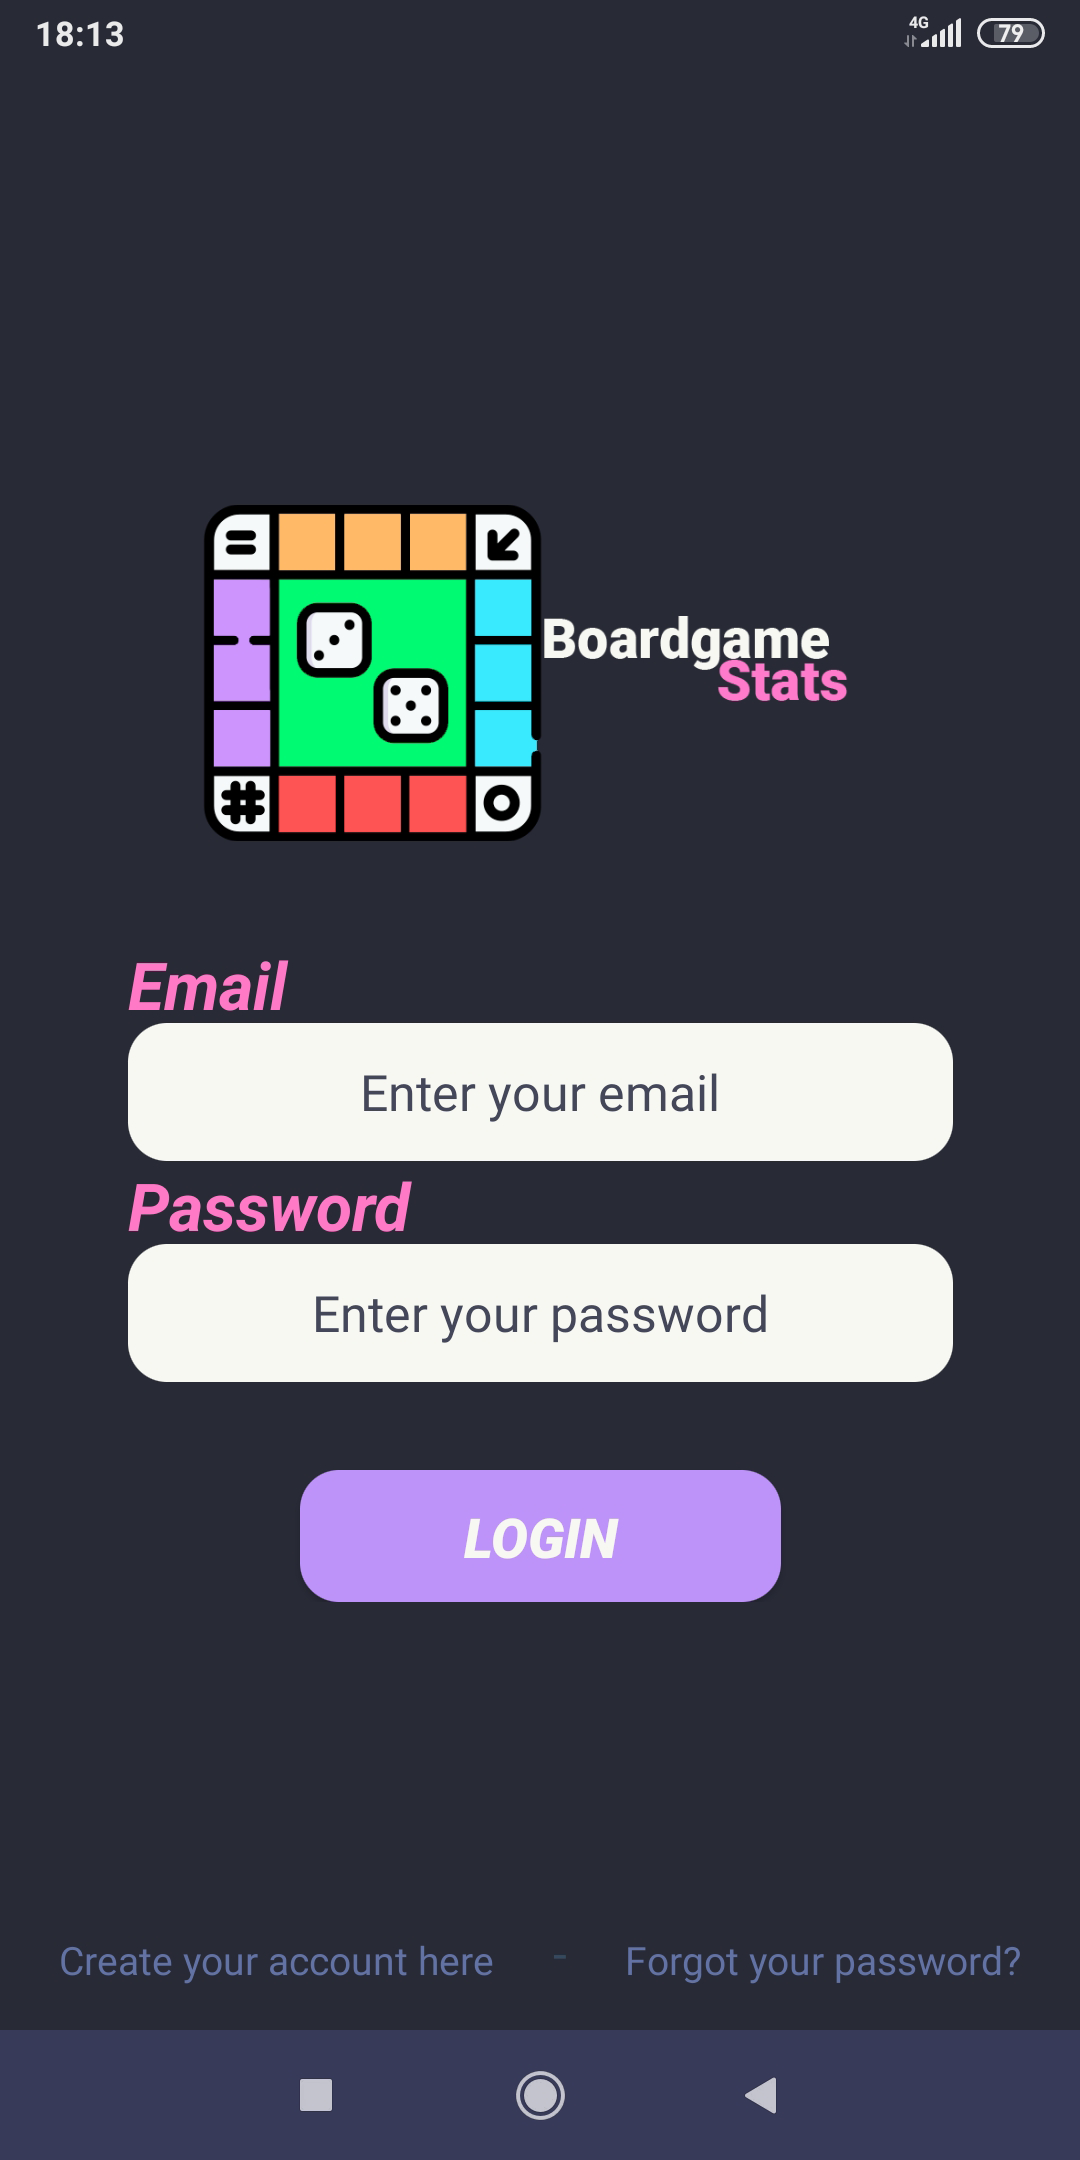
\includegraphics[width=0.3\linewidth]{fig/Uso/1.png}
    \caption{Inicio de sesión}
    \label{fig:uso1}
\end{figure}

Este no es el caso, por lo que primero deberemos registrarnos. Para ello vamos a pulsar el botón que se nos muestra reflejado en la siguiente figura.

\begin{figure}[H]
    \centering
    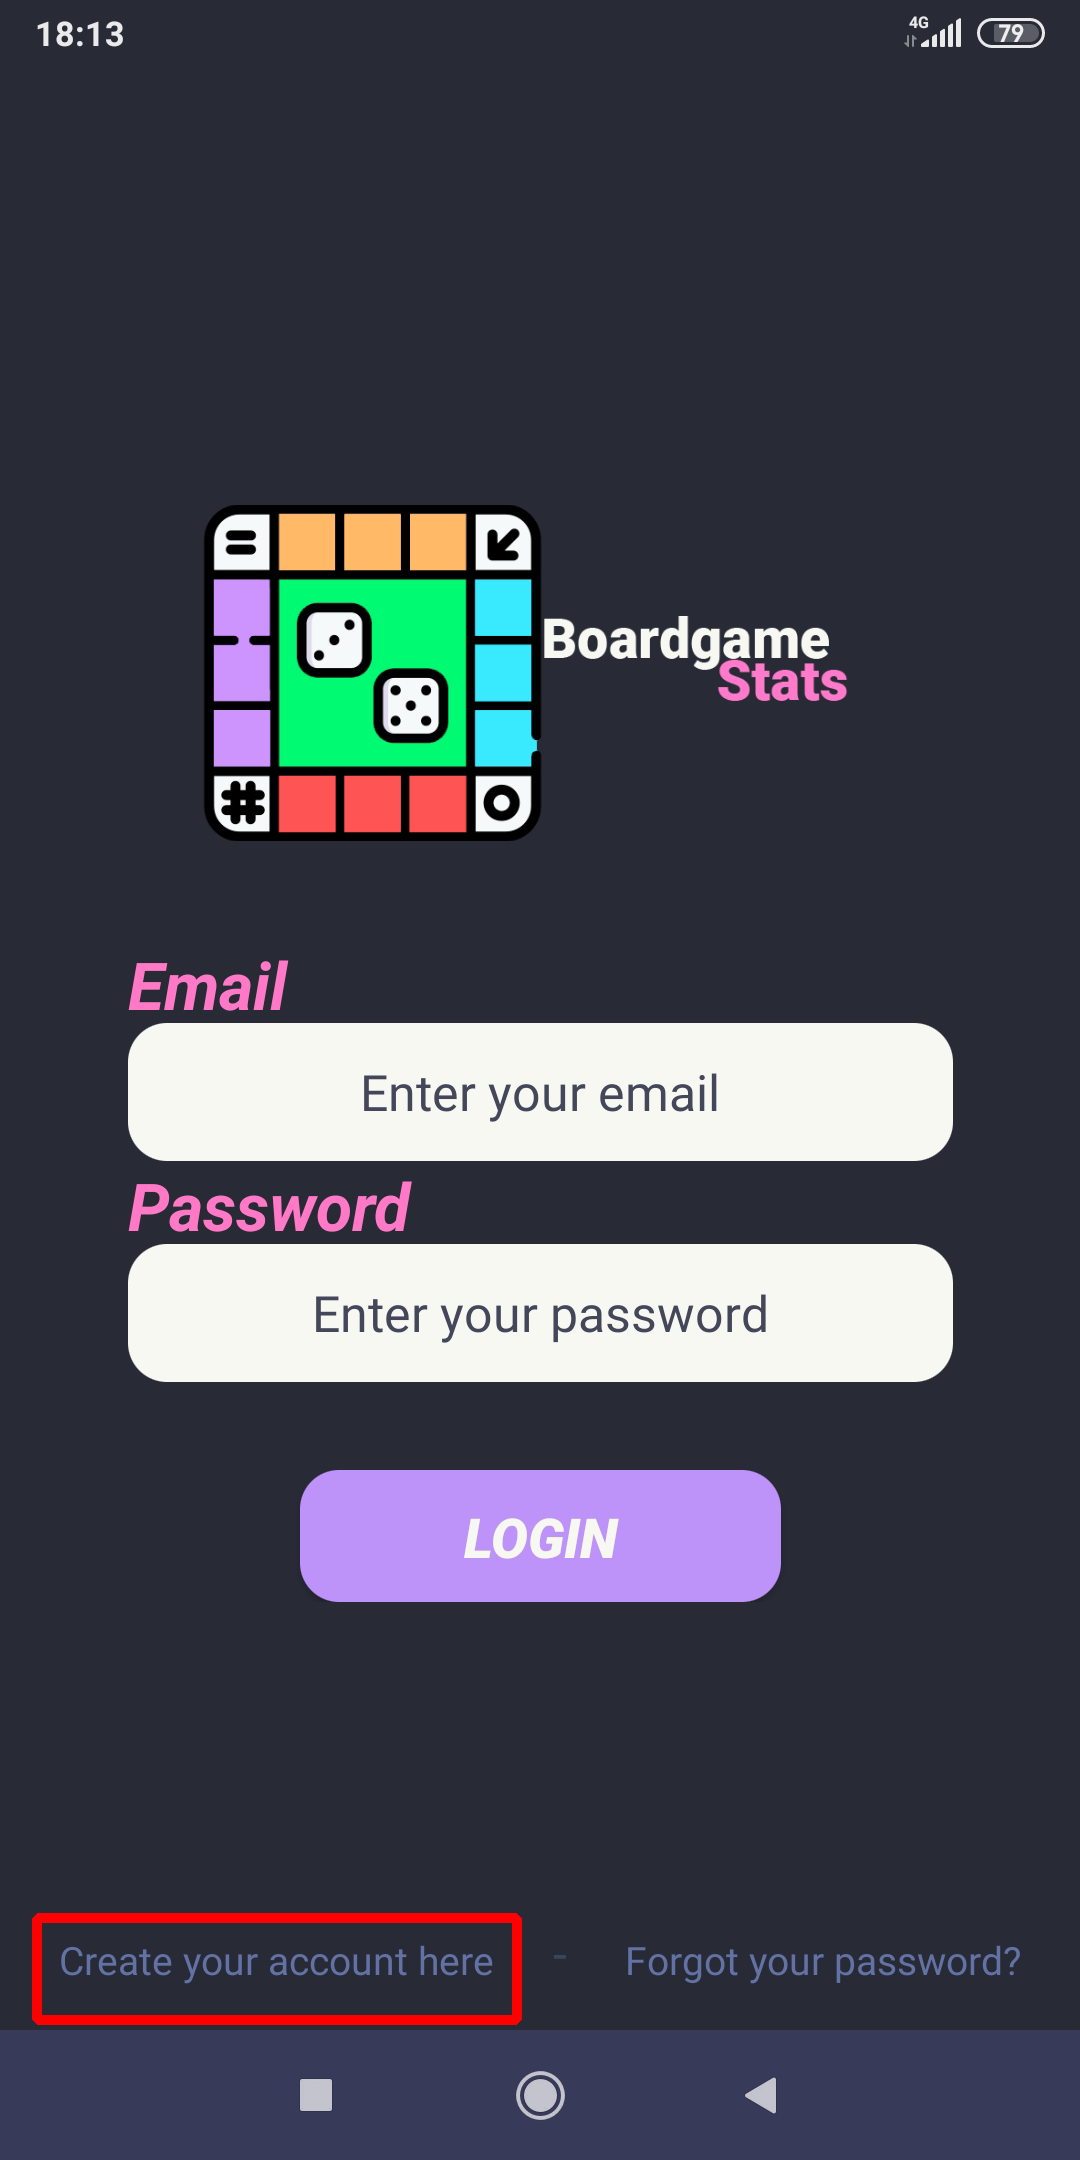
\includegraphics[width=0.3\linewidth]{fig/Uso/2.png}
    \caption{Iniciar registro}
    \label{fig:uso2}
\end{figure}

Una vez dentro de la actividad para registrarnos veremos algo como lo de ahora.

\begin{figure}[H]
    \centering
    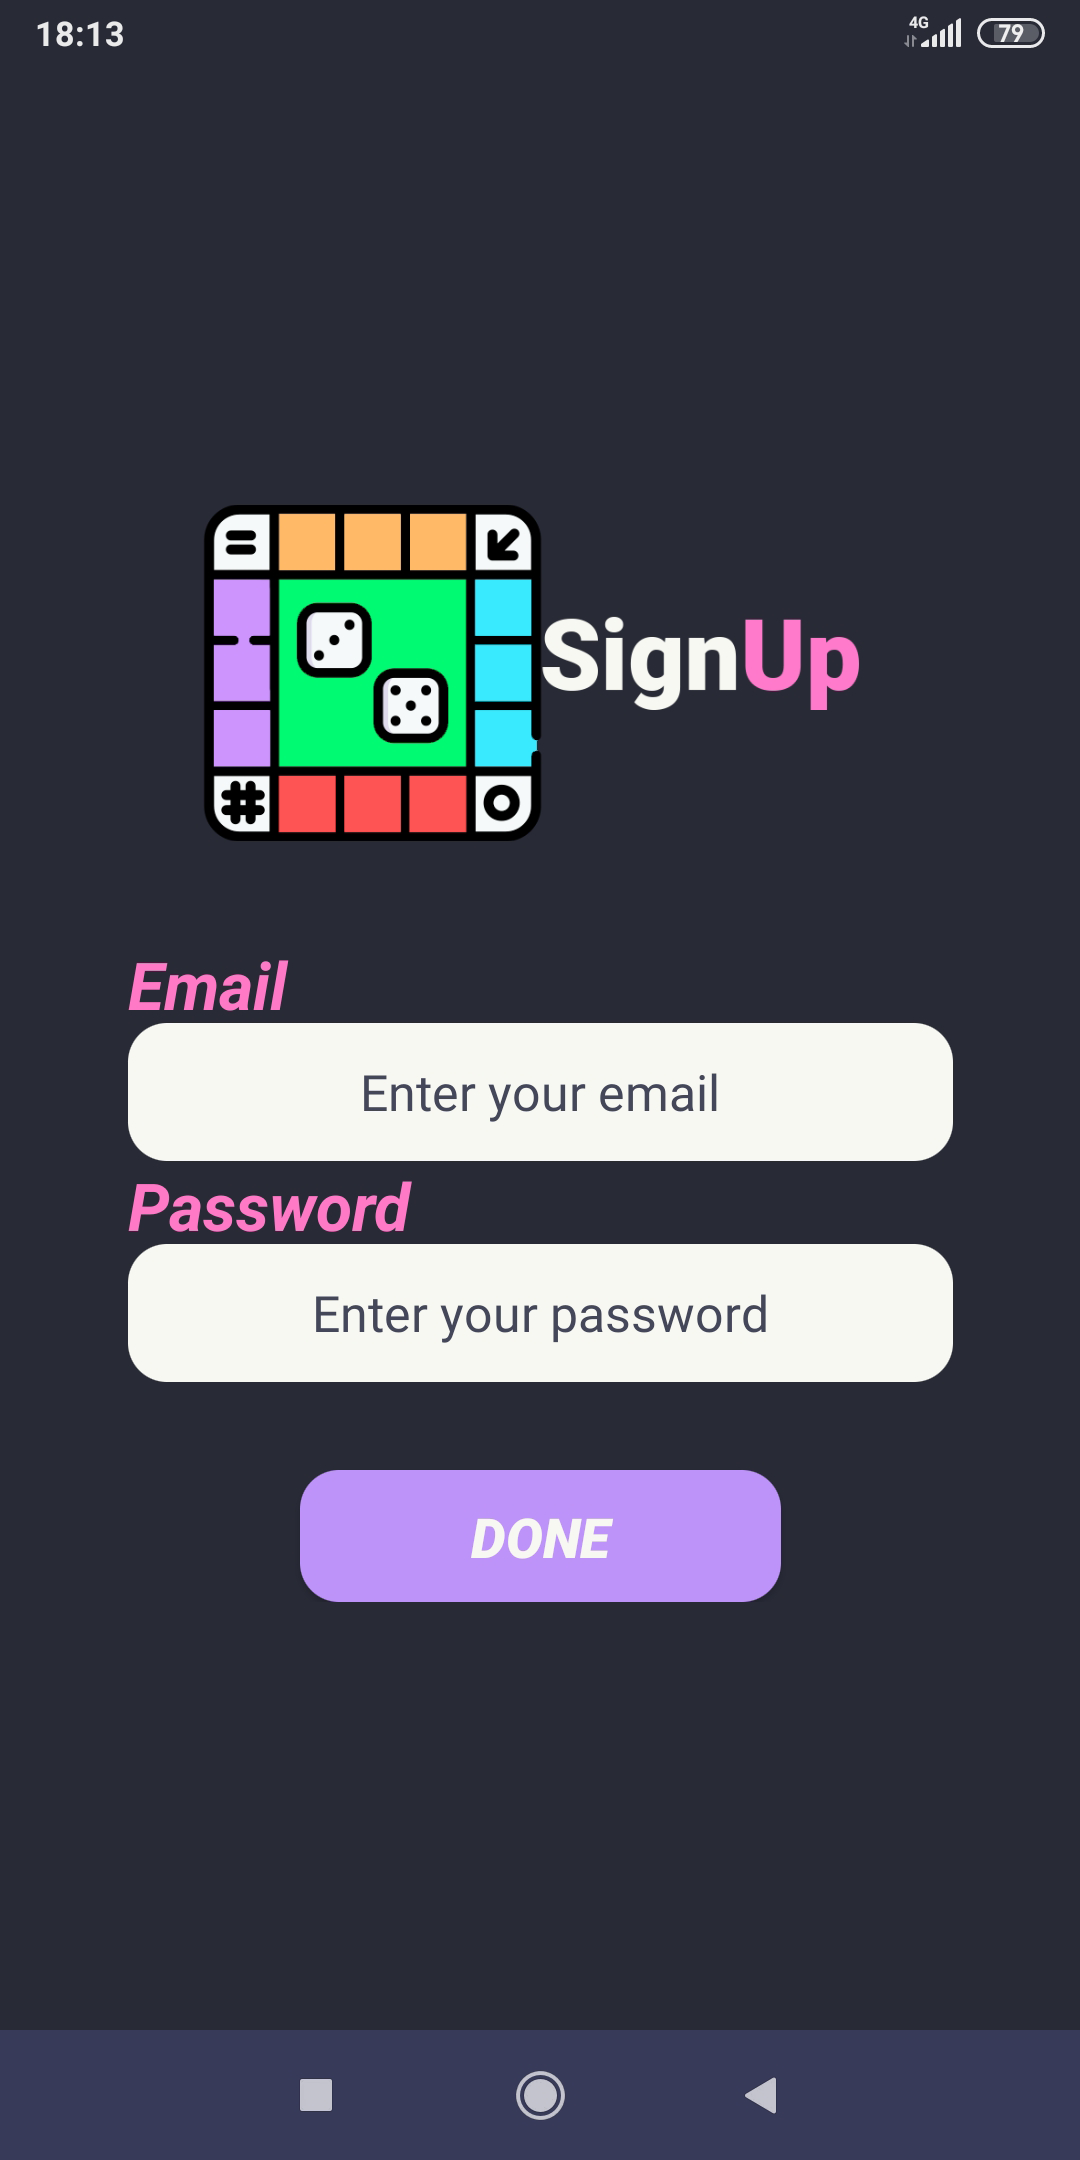
\includegraphics[width=0.3\linewidth]{fig/Uso/3.png}
    \caption{Registro}
    \label{fig:uso3}
\end{figure}

Donde tendremos que escibir nuestro correo y contraseña, y, por último, clicar en el botón que pone \textit{Done}.

\begin{figure}[H]
    \centering
    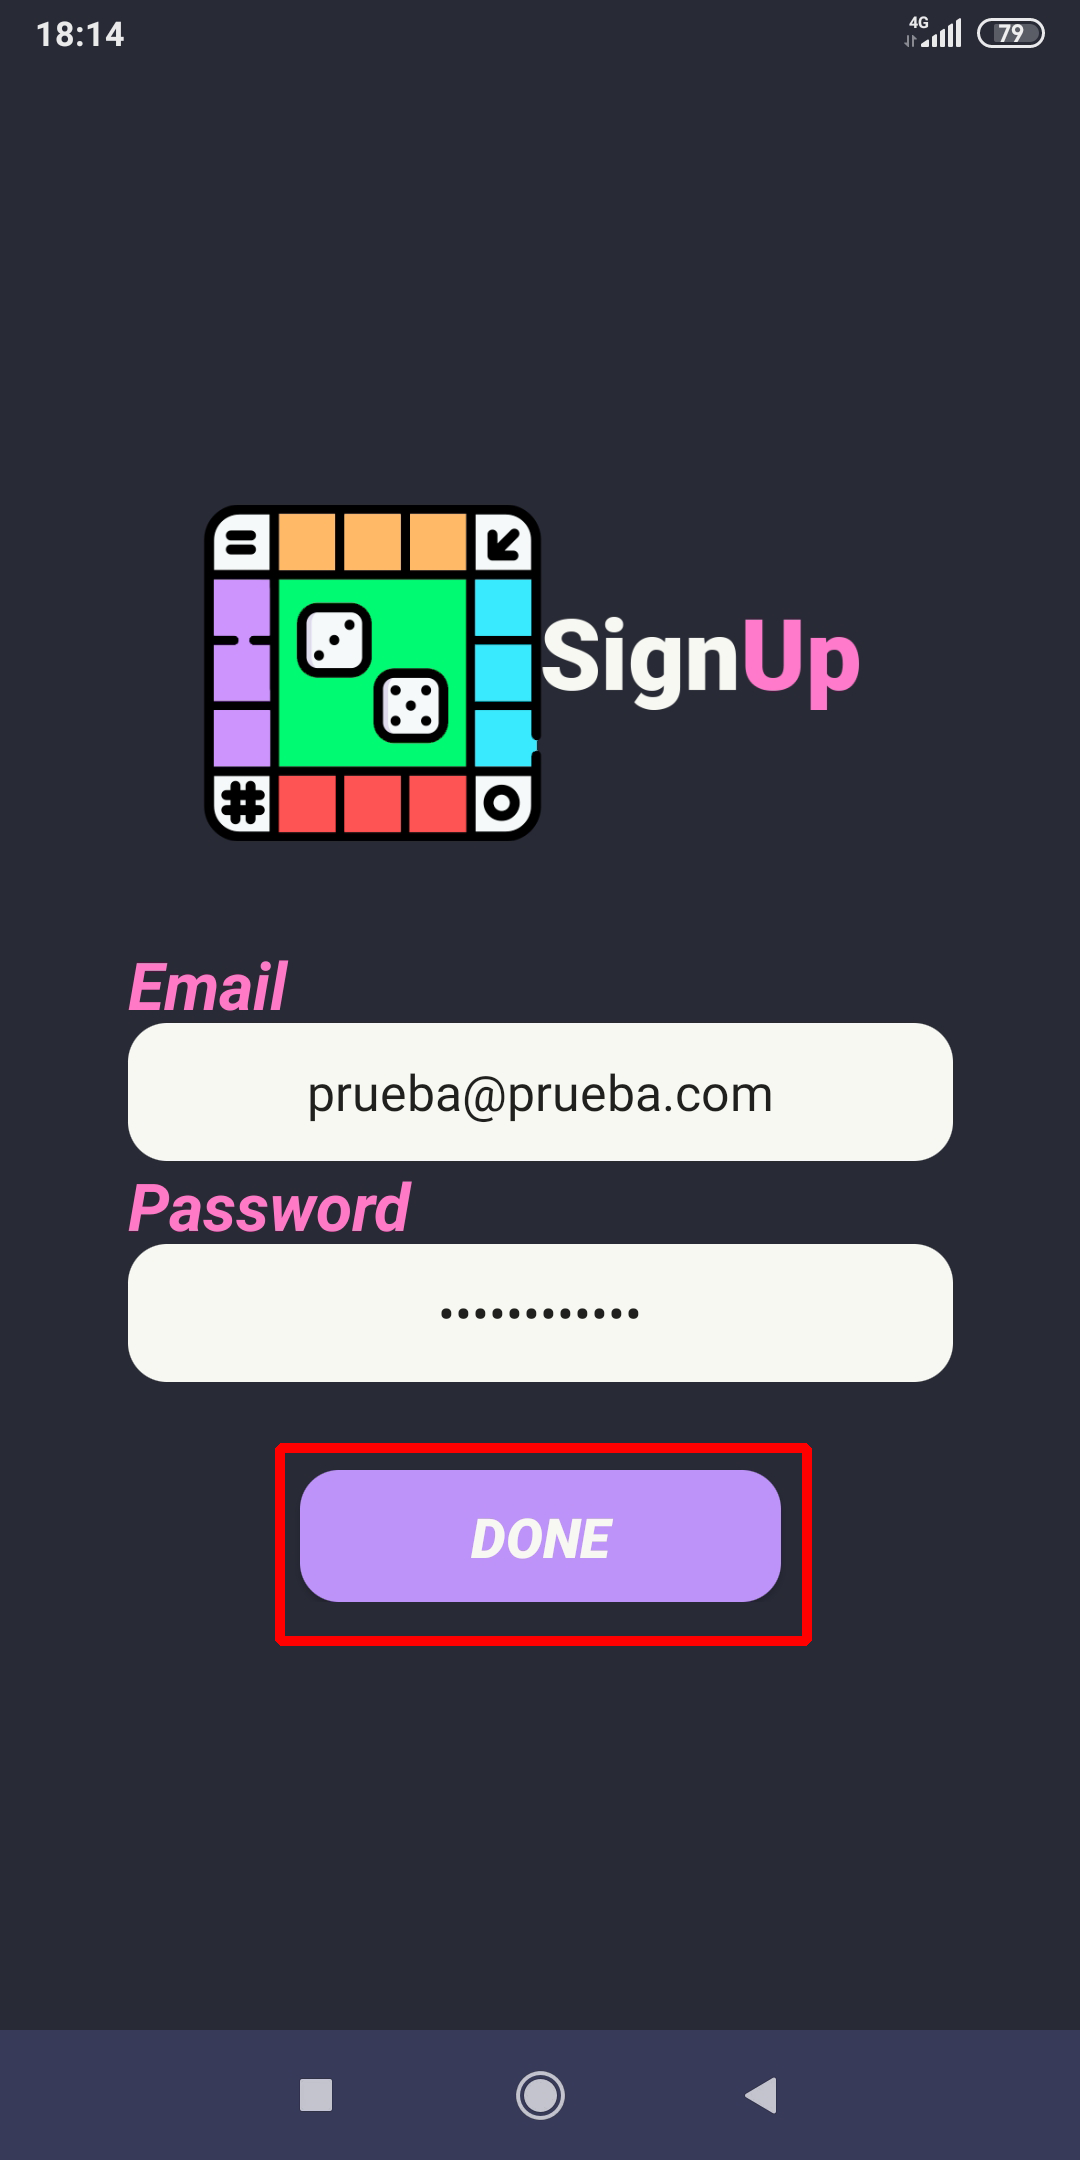
\includegraphics[width=0.3\linewidth]{fig/Uso/4.png}
    \caption{Completar registro}
    \label{fig:uso4}
\end{figure}

También, estando en la ventana de inicio de sesión, podremos clicar sobre el texto que pone \textit{Forgot your password?}, el cual nos abrirá el siguiente pop-up, donde podremos escribir nuestro correo electrónico para que nos haga llegar un correo para restablecer la contraseña.

\begin{figure}[H]
    \centering
    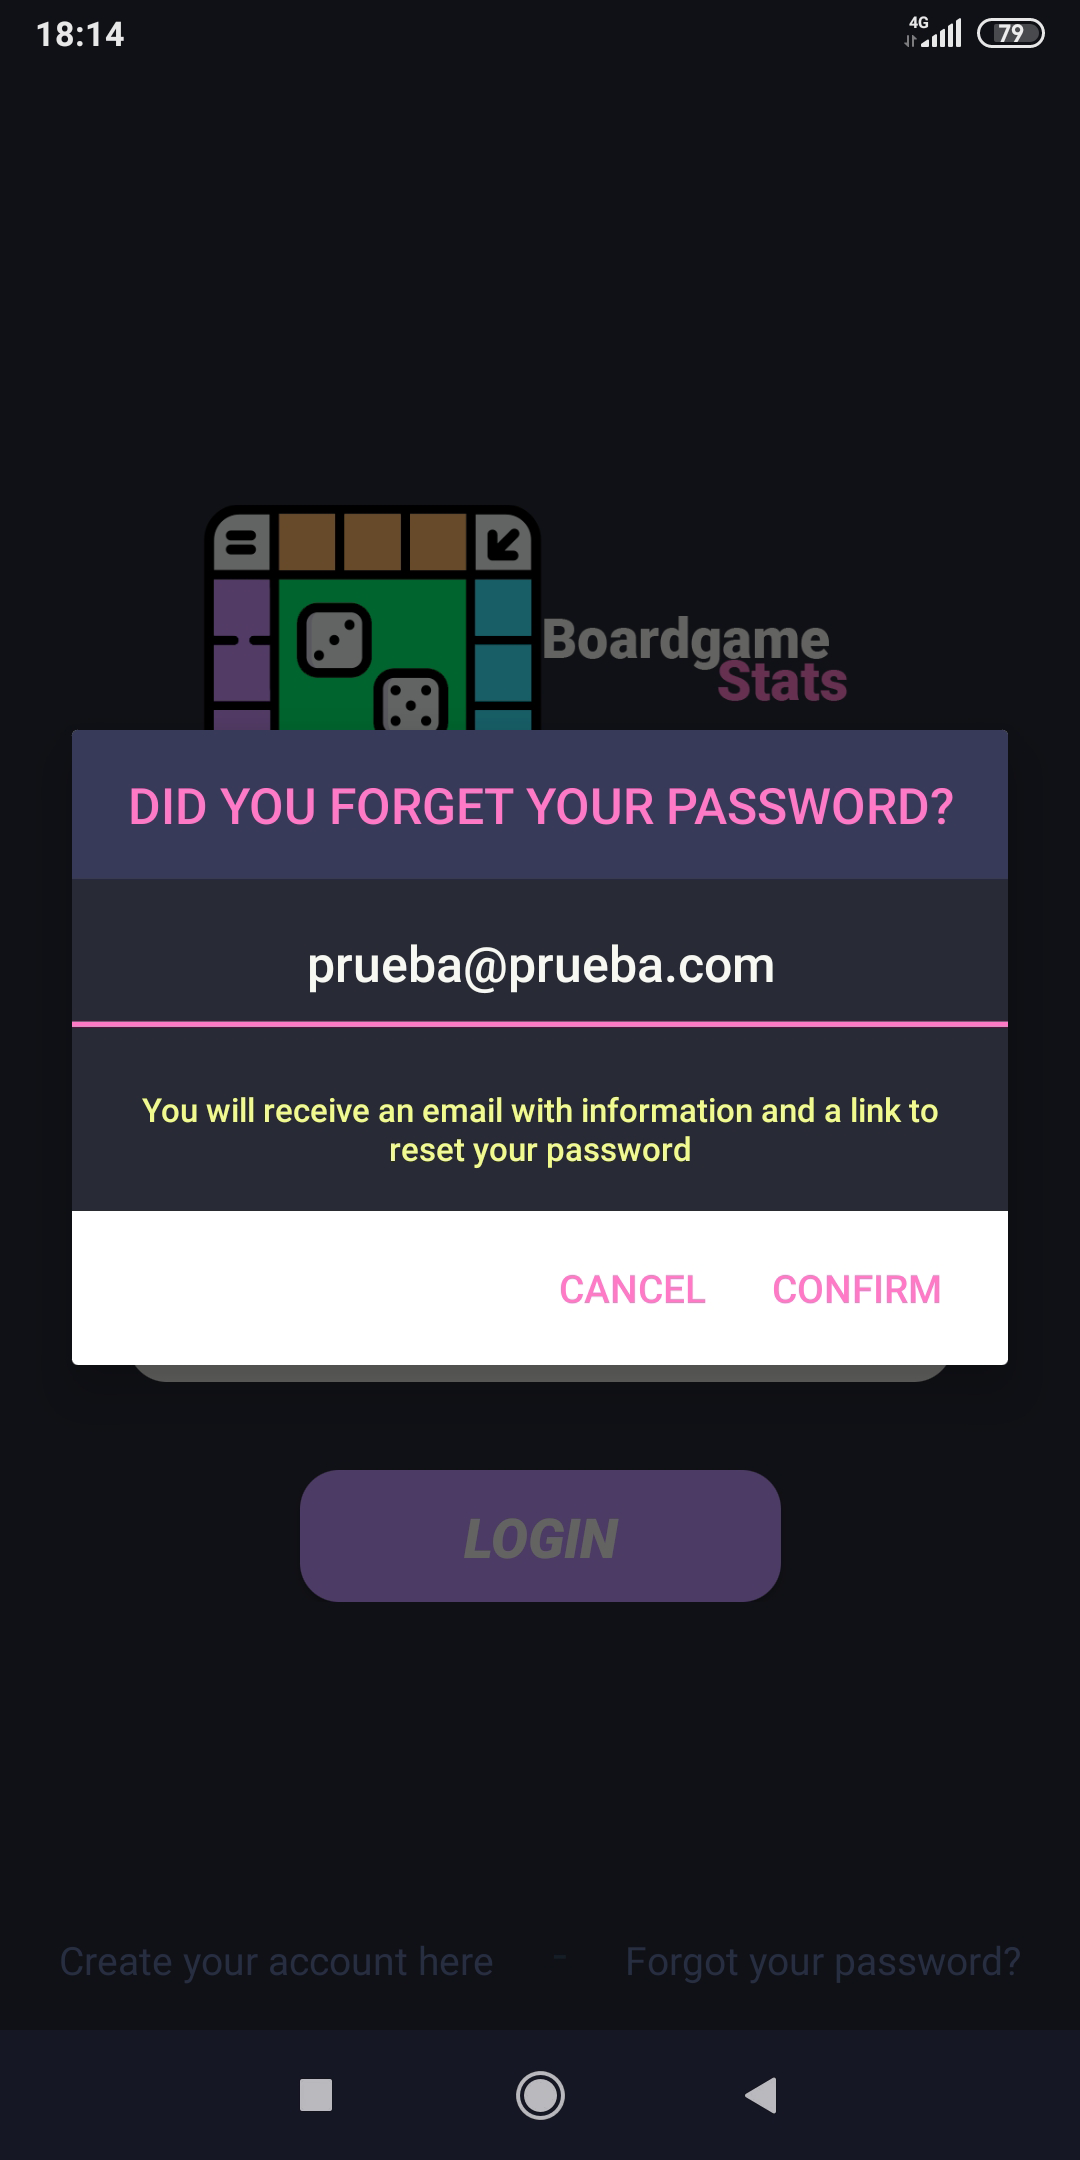
\includegraphics[width=0.3\linewidth]{fig/Uso/5.png}
    \caption{¿Olvidaste la contraseña?}
    \label{fig:uso5}
\end{figure}

Una vez estemos ya registrados, usaremos dicha cuenta para iniciar sesión en la aplicación.

\begin{figure}[H]
    \centering
    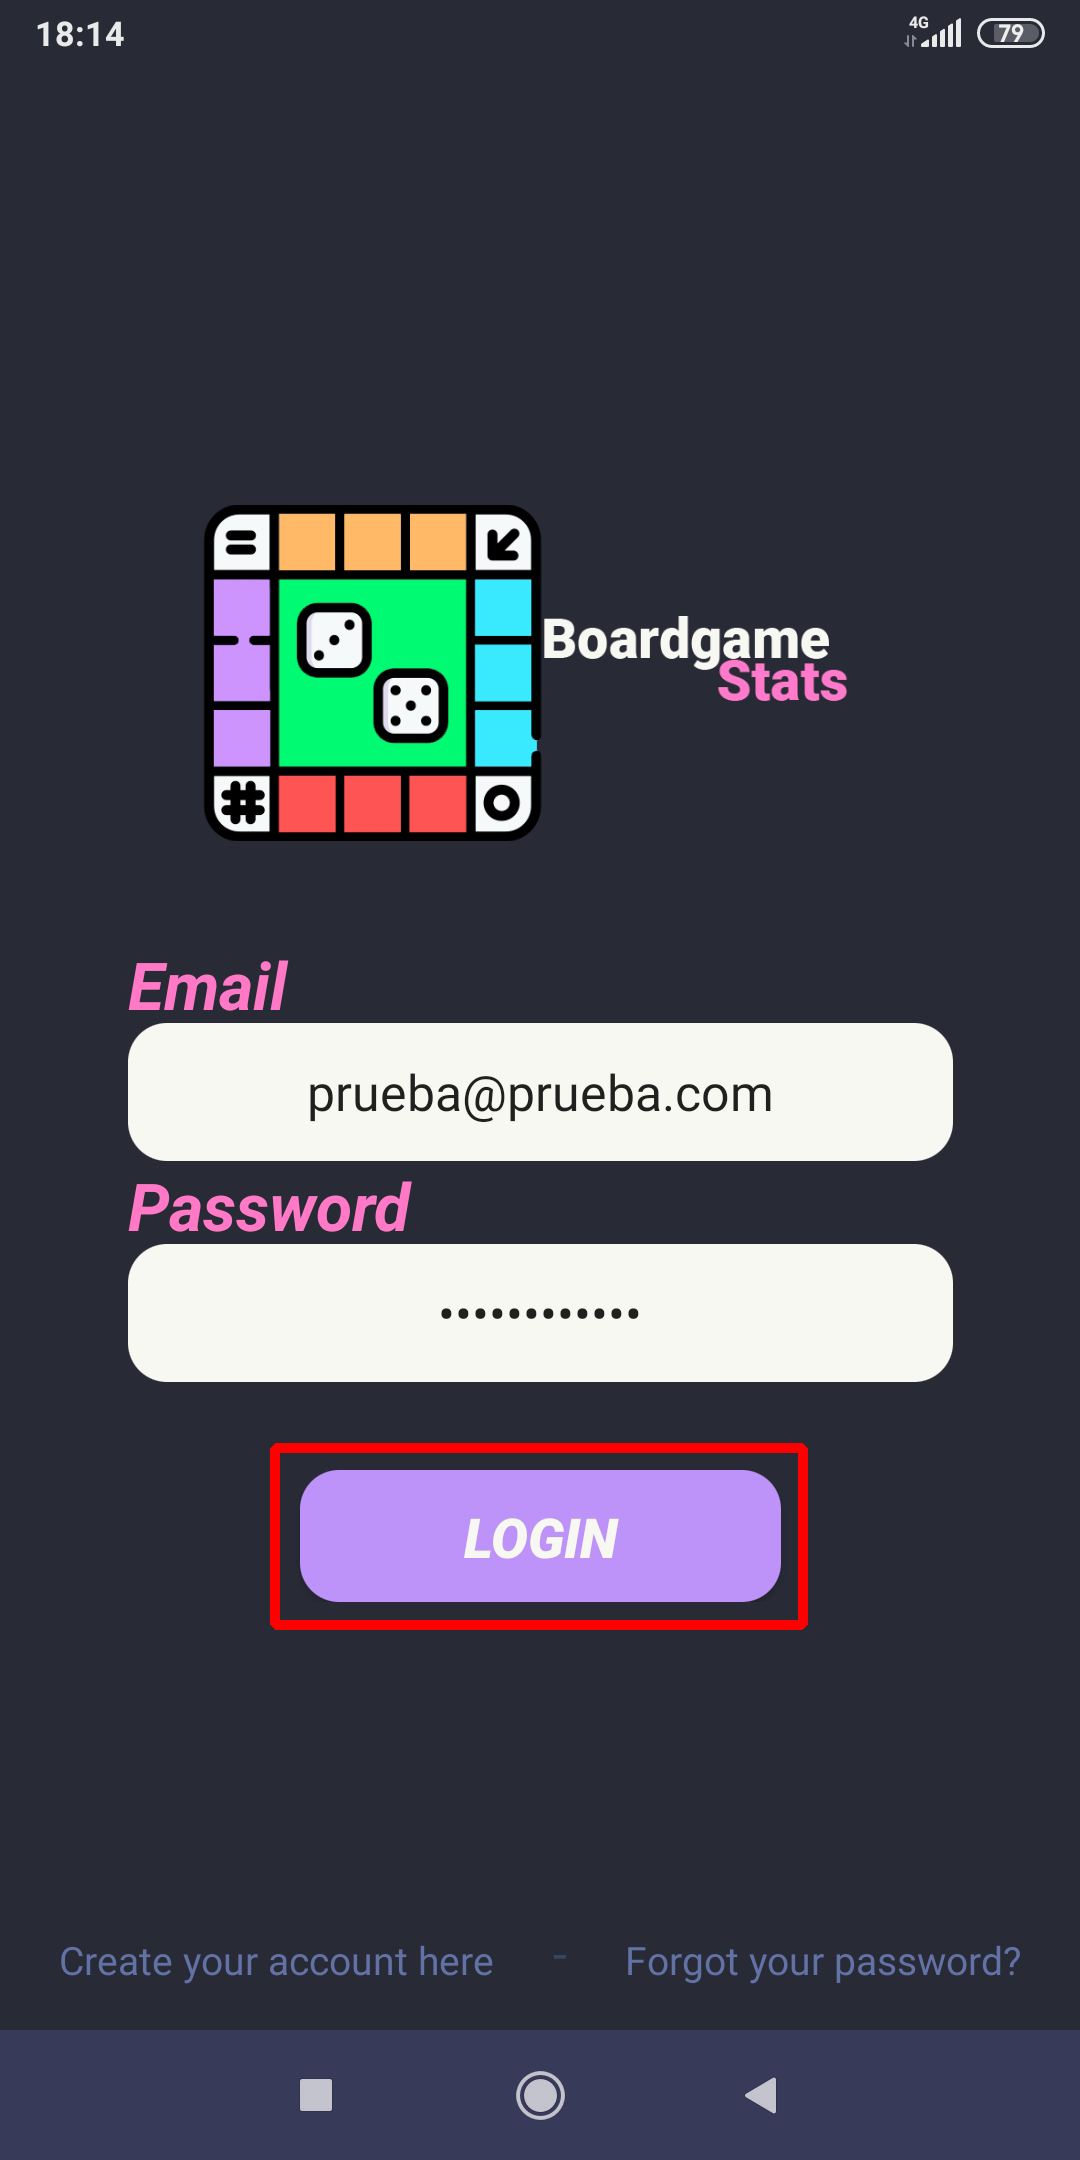
\includegraphics[width=0.3\linewidth]{fig/Uso/6.png}
    \caption{Inicio sesión completado}
    \label{fig:uso6}
\end{figure}

Con la sesión ya iniciada, lo primero que veremos será esta ventana en la que tendremos una lista vacía o con juegos que vayamos seleccionando de uno en uno, un texto con el que accederemos a la actividad para seleccionar dichos juegos, y una barra de navegación en la zona inferior de la ventana.

\begin{figure}[H]
    \centering
    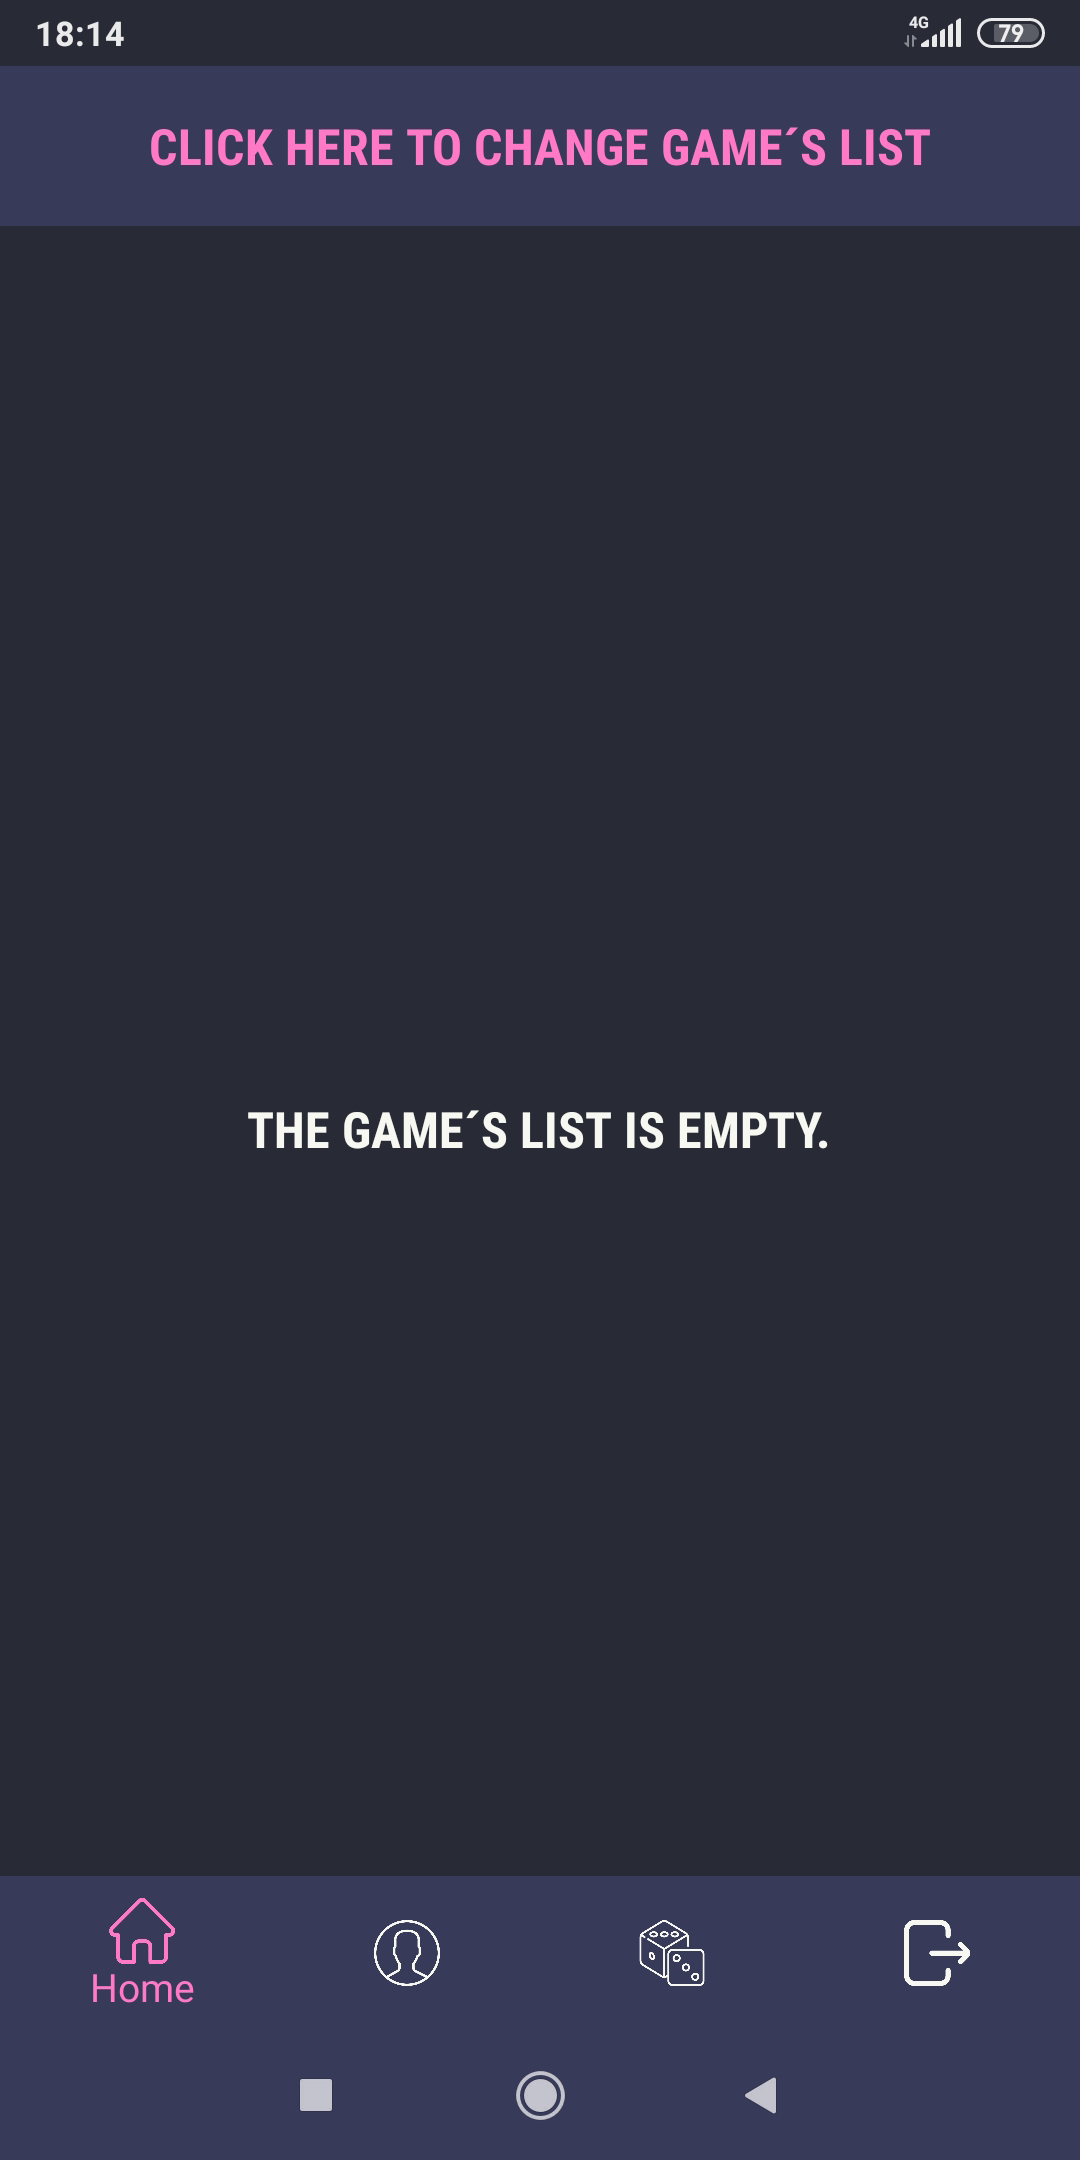
\includegraphics[width=0.3\linewidth]{fig/Uso/7.png}
    \caption{Actividad Home con lista vacía}
    \label{fig:uso7}
\end{figure}

\begin{figure}[H]
    \centering
    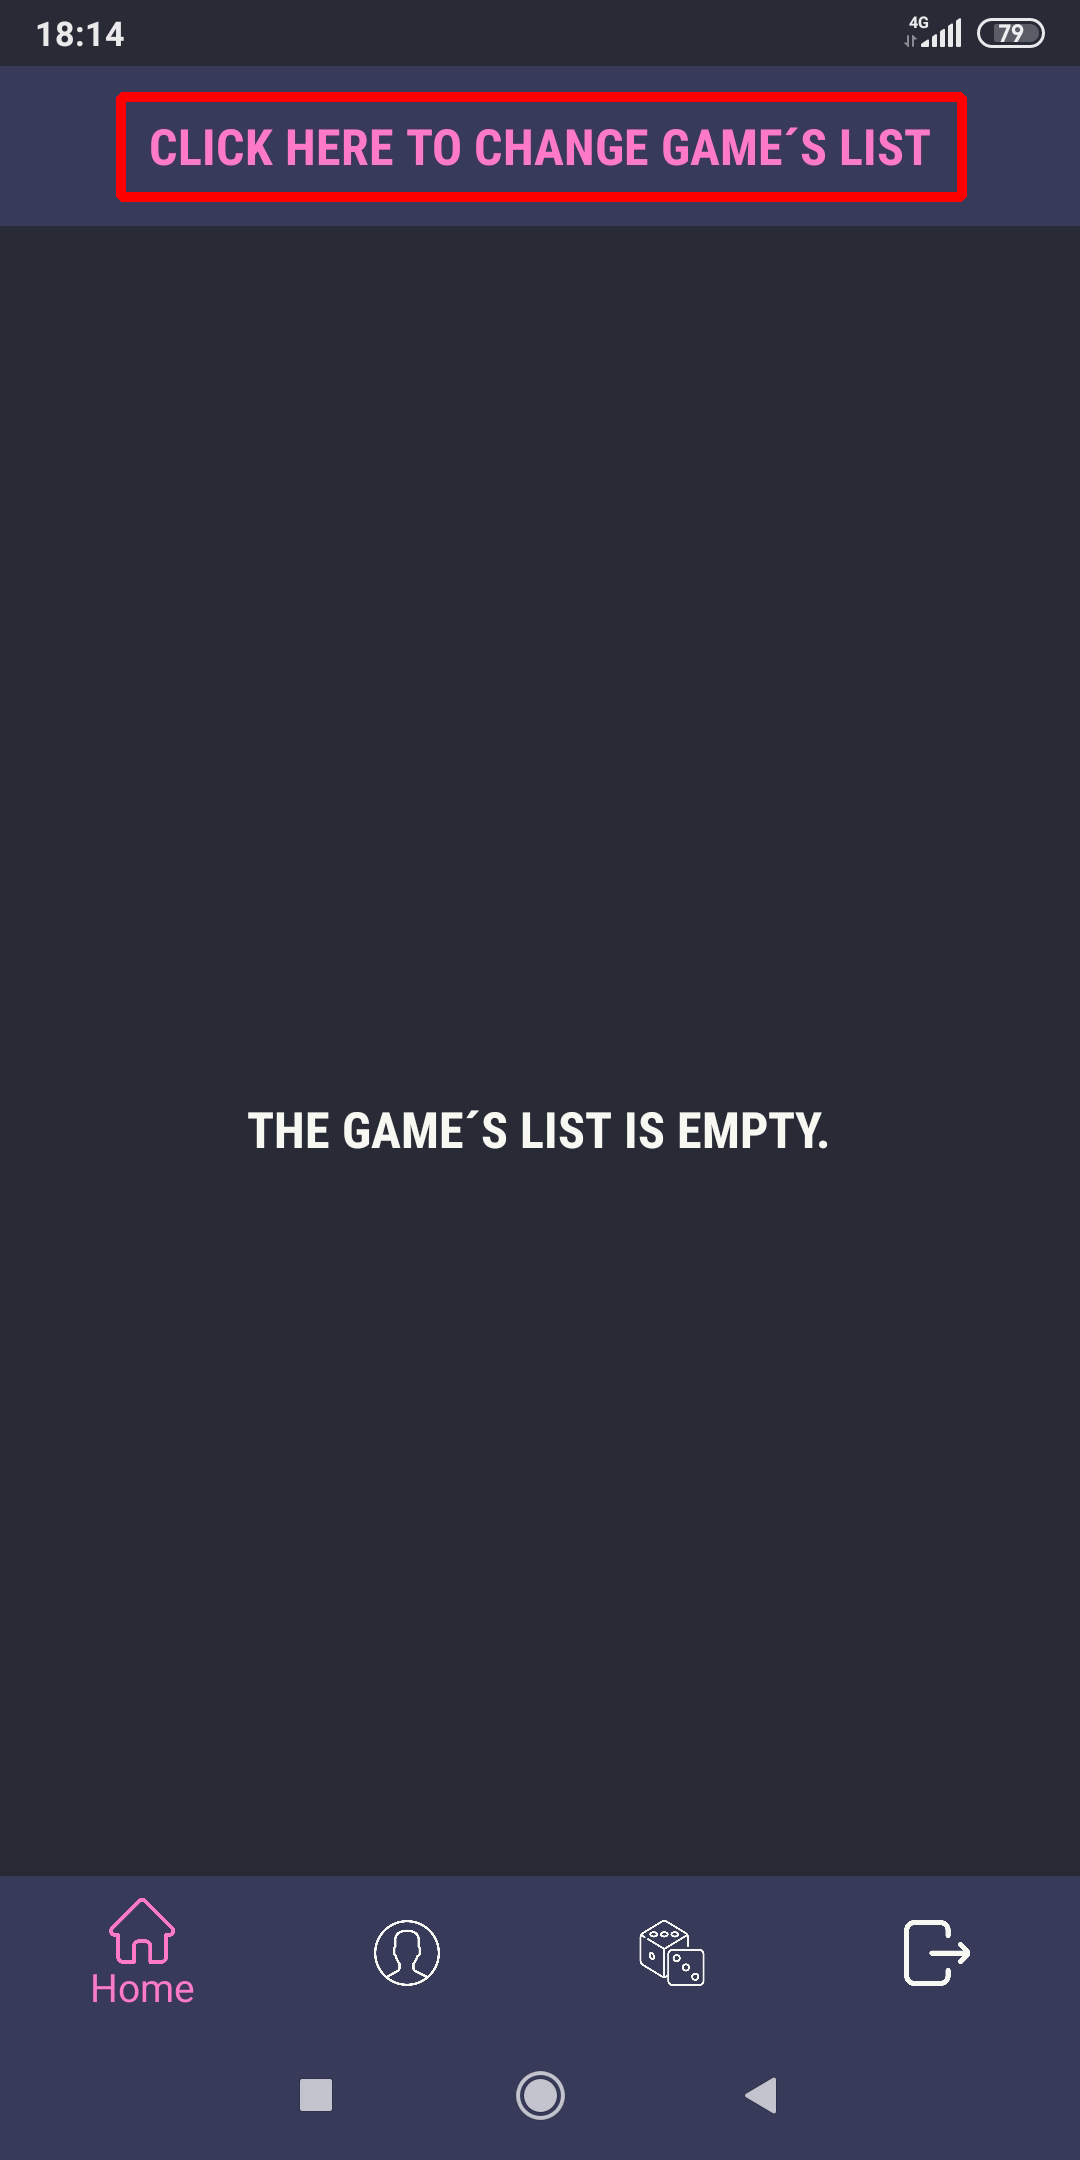
\includegraphics[width=0.3\linewidth]{fig/Uso/8.png}
    \caption{Texto para seleccionar juegos}
    \label{fig:uso8}
\end{figure}

\begin{figure}[H]
    \centering
    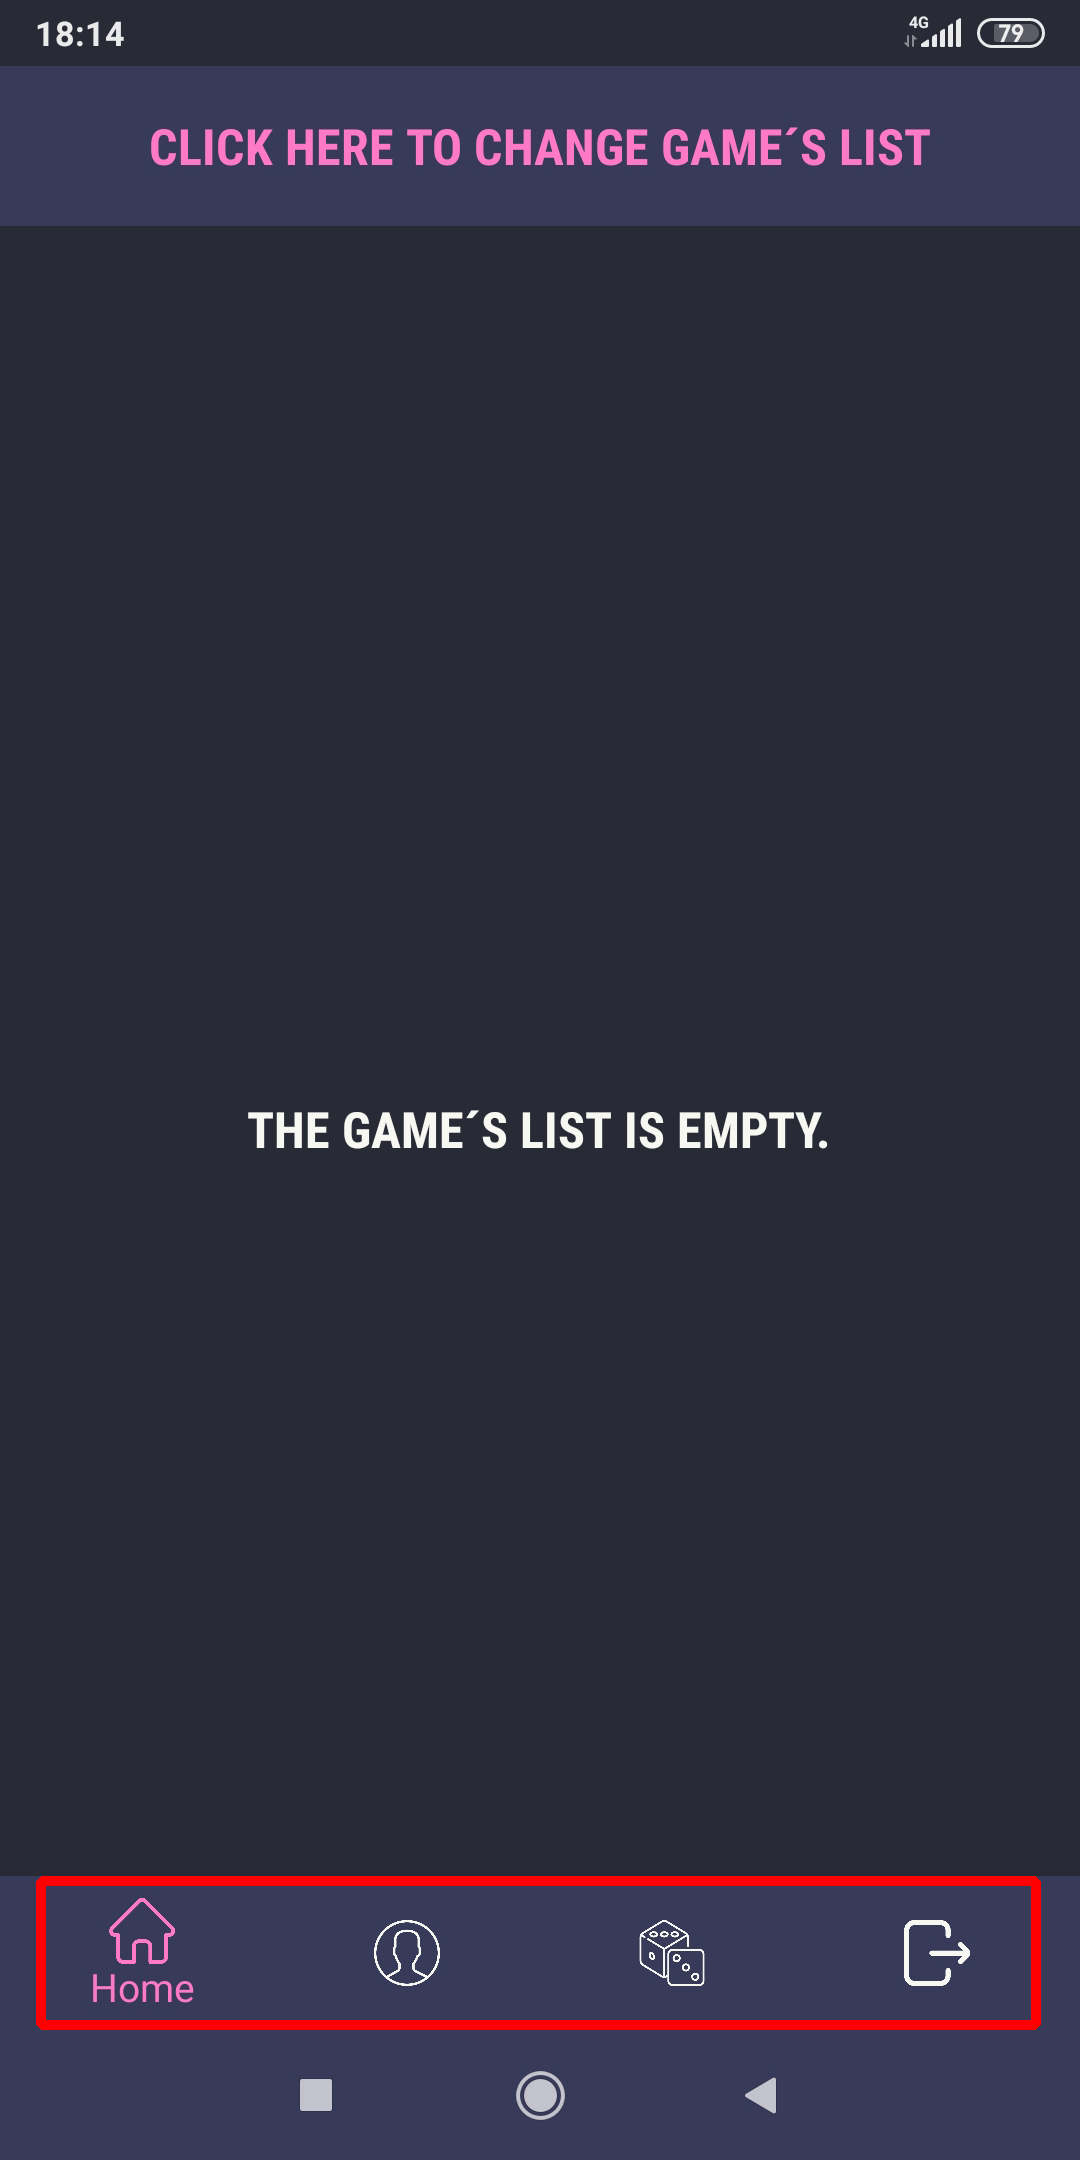
\includegraphics[width=0.3\linewidth]{fig/Uso/9.png}
    \caption{Barra de navegación}
    \label{fig:uso9}
\end{figure}

Si entramos en la actividad para seleccionar juegos, nos encontraremos con una barra de búsqueda

\begin{figure}[H]
    \centering
    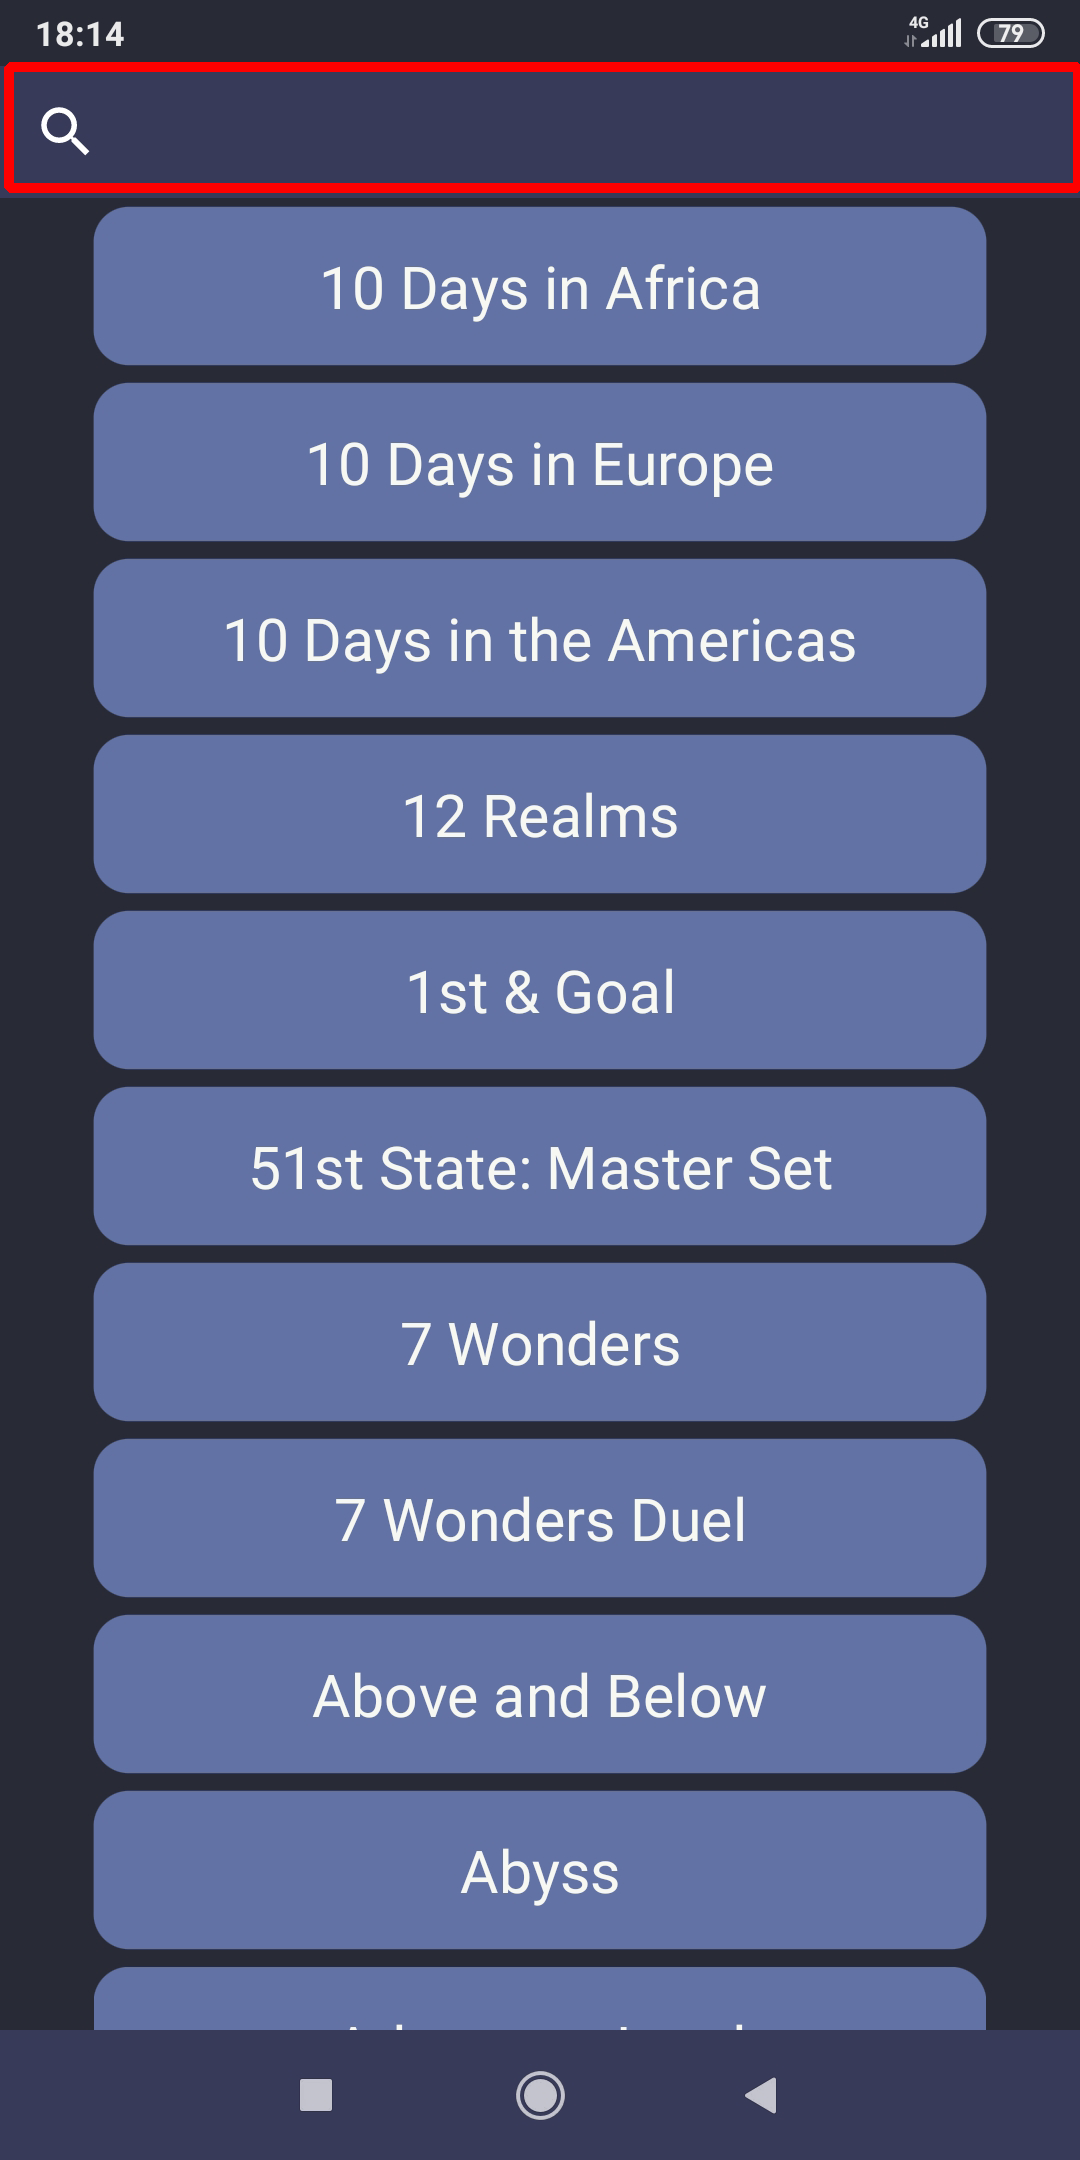
\includegraphics[width=0.3\linewidth]{fig/Uso/10.png}
    \caption{Barra de búsqueda de juegos}
    \label{fig:uso10}
\end{figure}

y una lista rellena de juegos de mesa sacados de una API en la que se puede hacer scroll.

\begin{figure}[H]
    \centering
    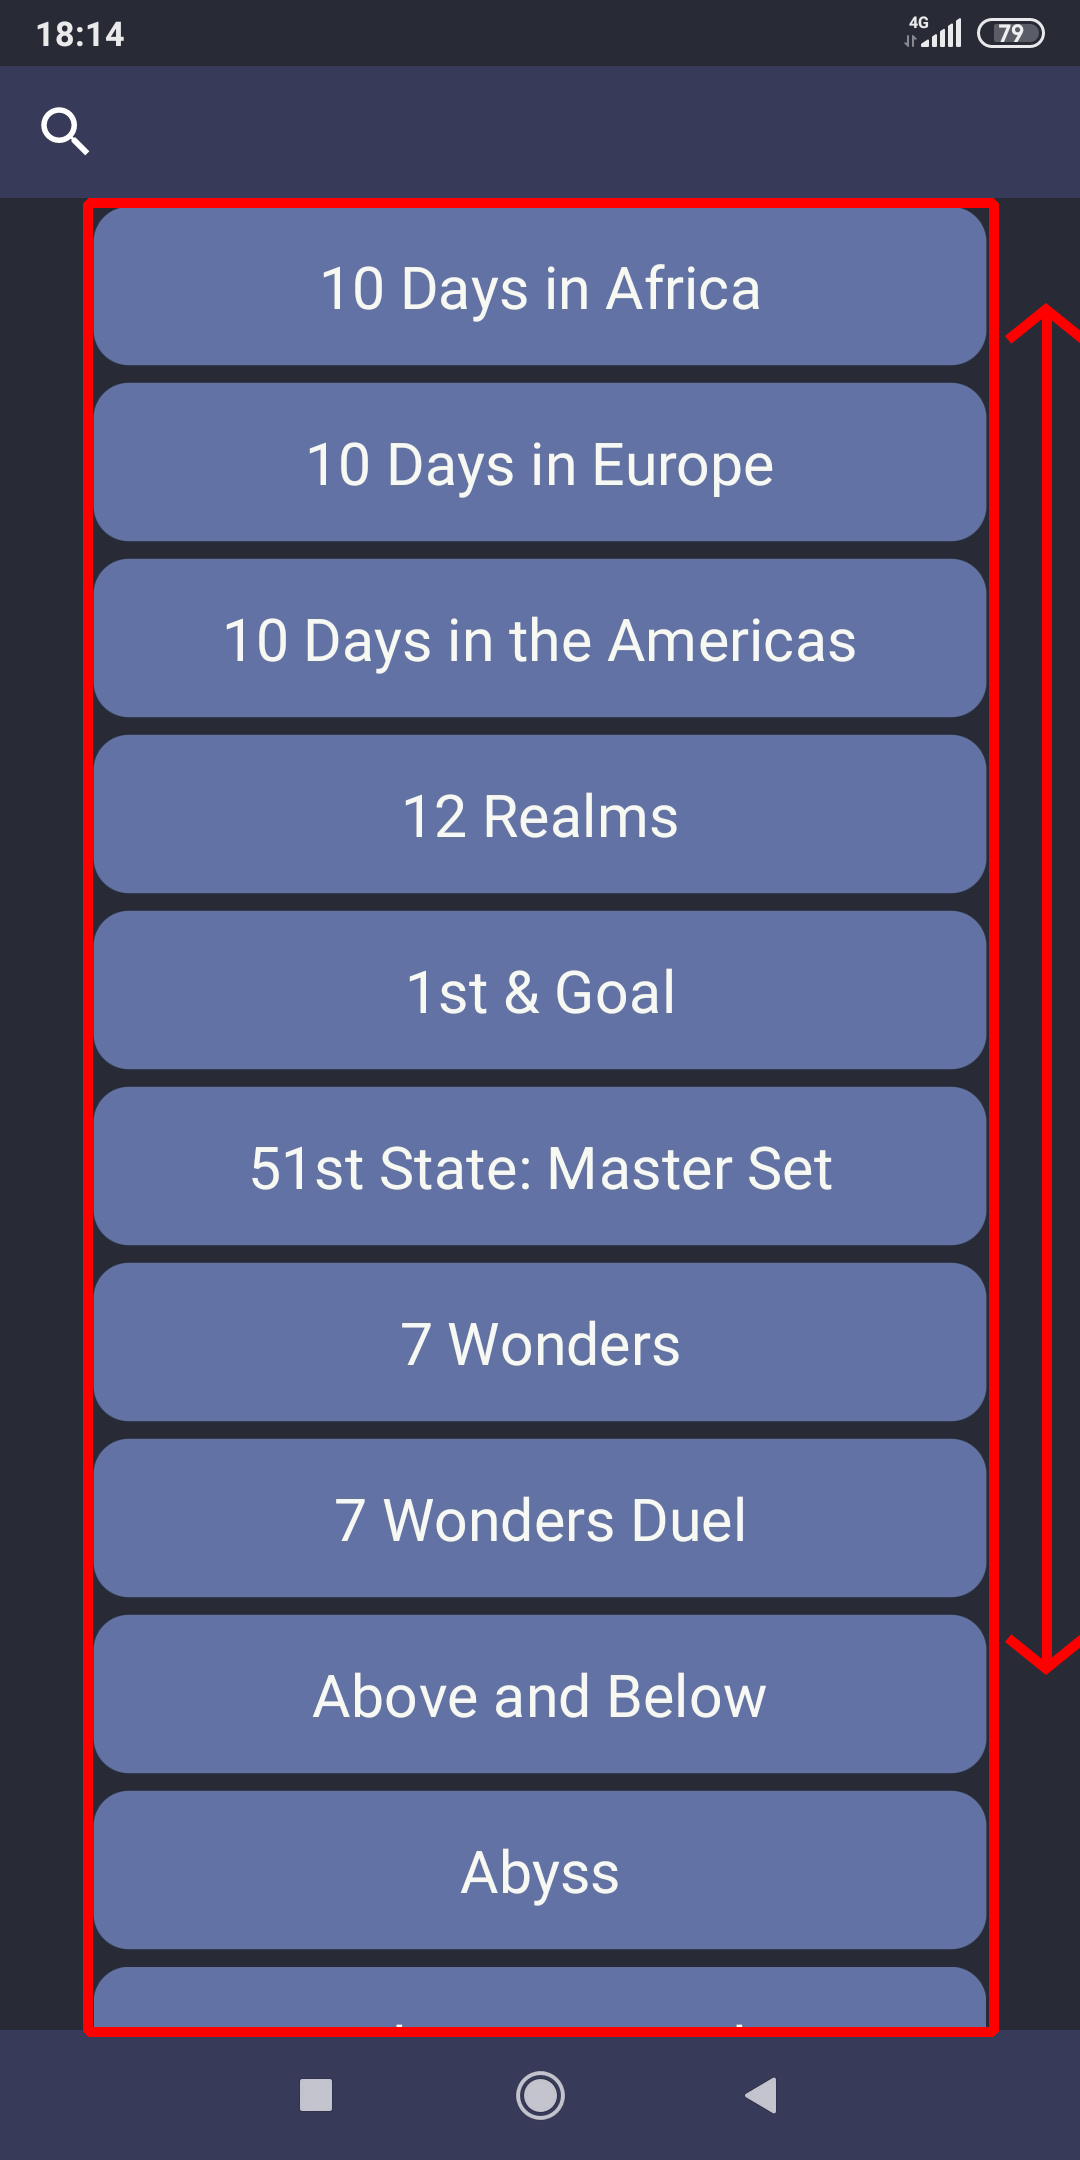
\includegraphics[width=0.3\linewidth]{fig/Uso/11.png}
    \caption{Lista de juegos completa}
    \label{fig:uso11}
\end{figure}

Cuando seleccionamos un juego de esta lista, veremos las estadísticas que tengamos en ese juego de mesa y un botón con el que podremos agregar dicho juego a nuestra lista de juegos favoritos haciendo que aparezca en la lista de la actividad principal y un mensaje notificándonos de esto.

\begin{figure}[H]
    \centering
    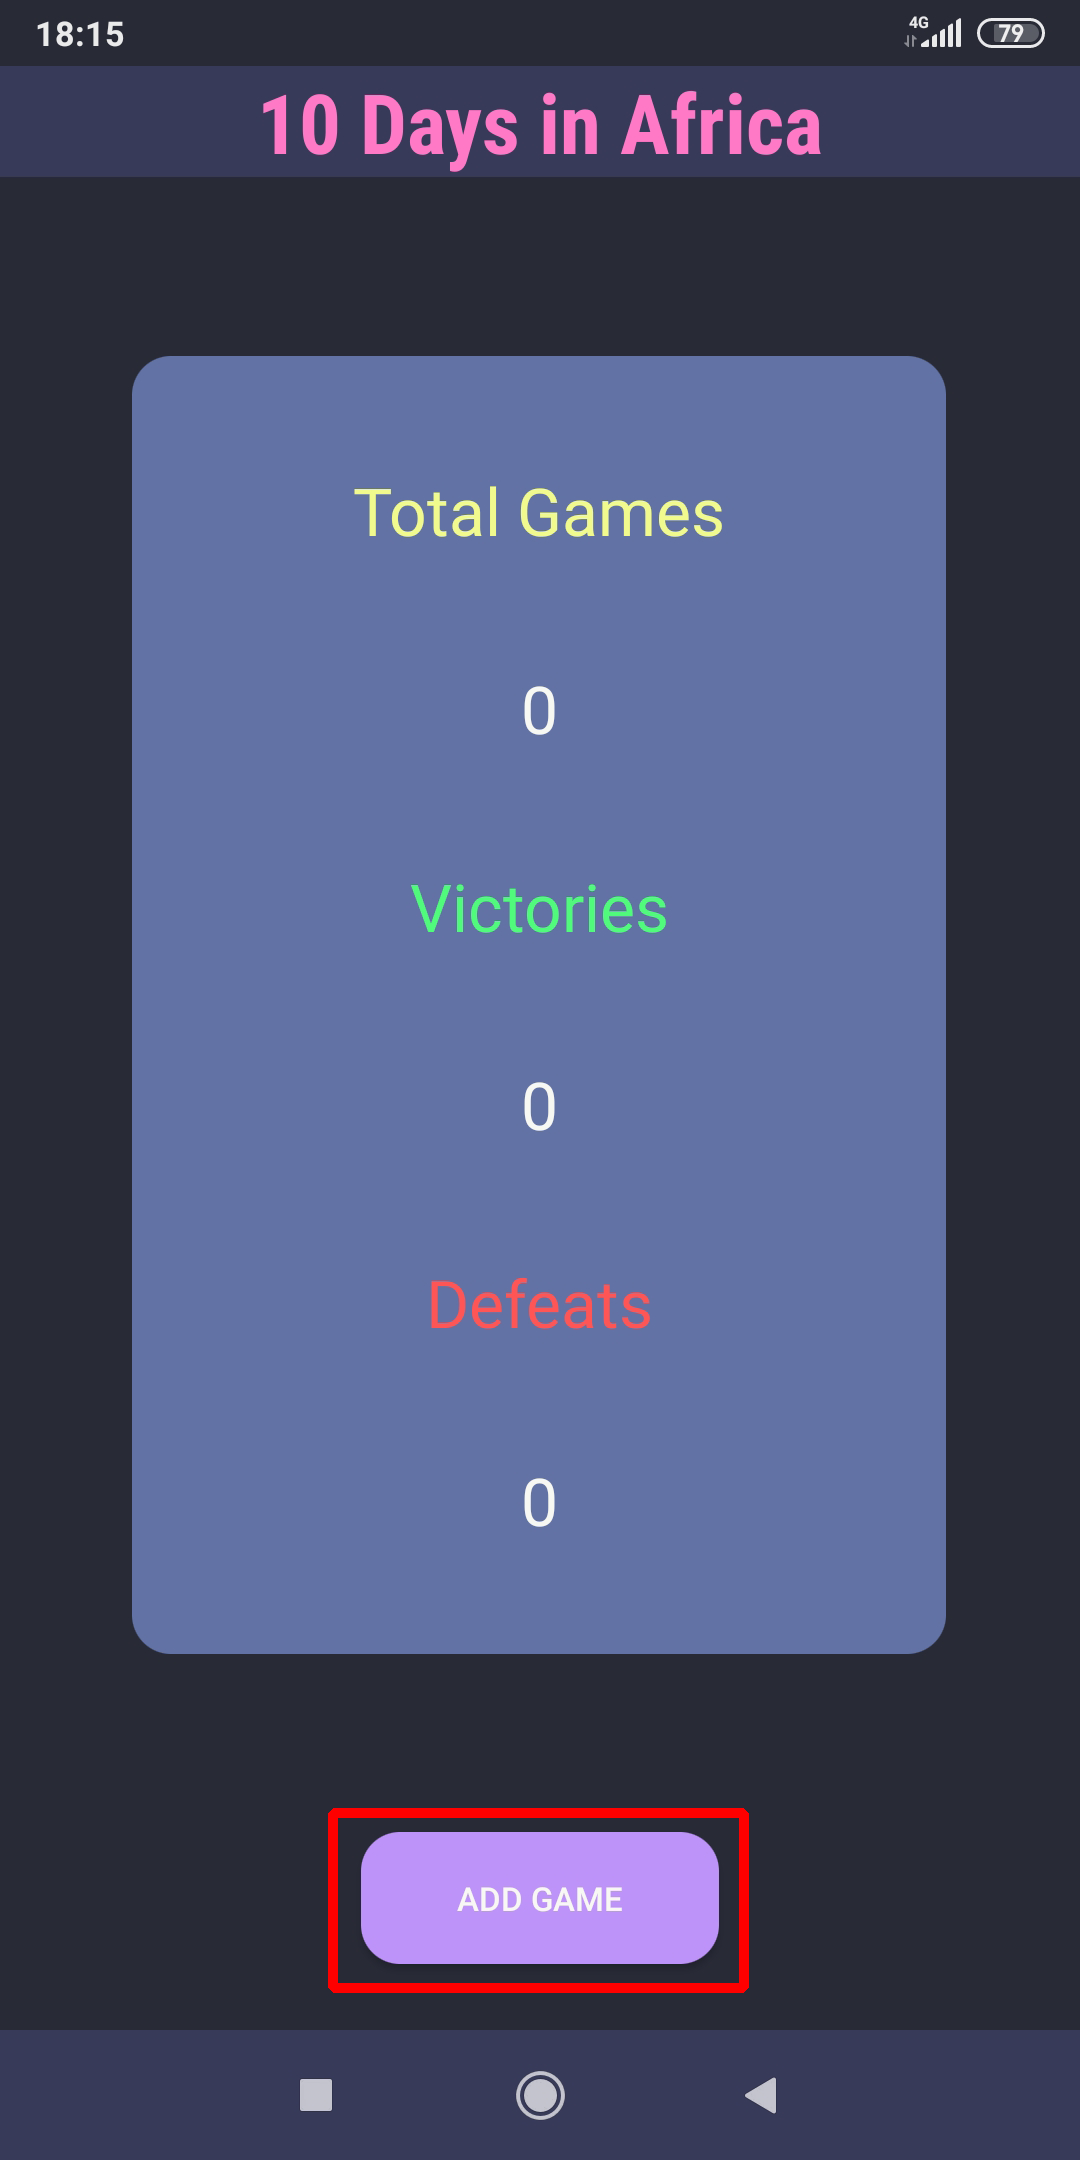
\includegraphics[width=0.3\linewidth]{fig/Uso/12.png}
    \caption{Añadir juego a lista de juegos favoritos}
    \label{fig:uso12}
\end{figure}

\begin{figure}[H]
    \centering
    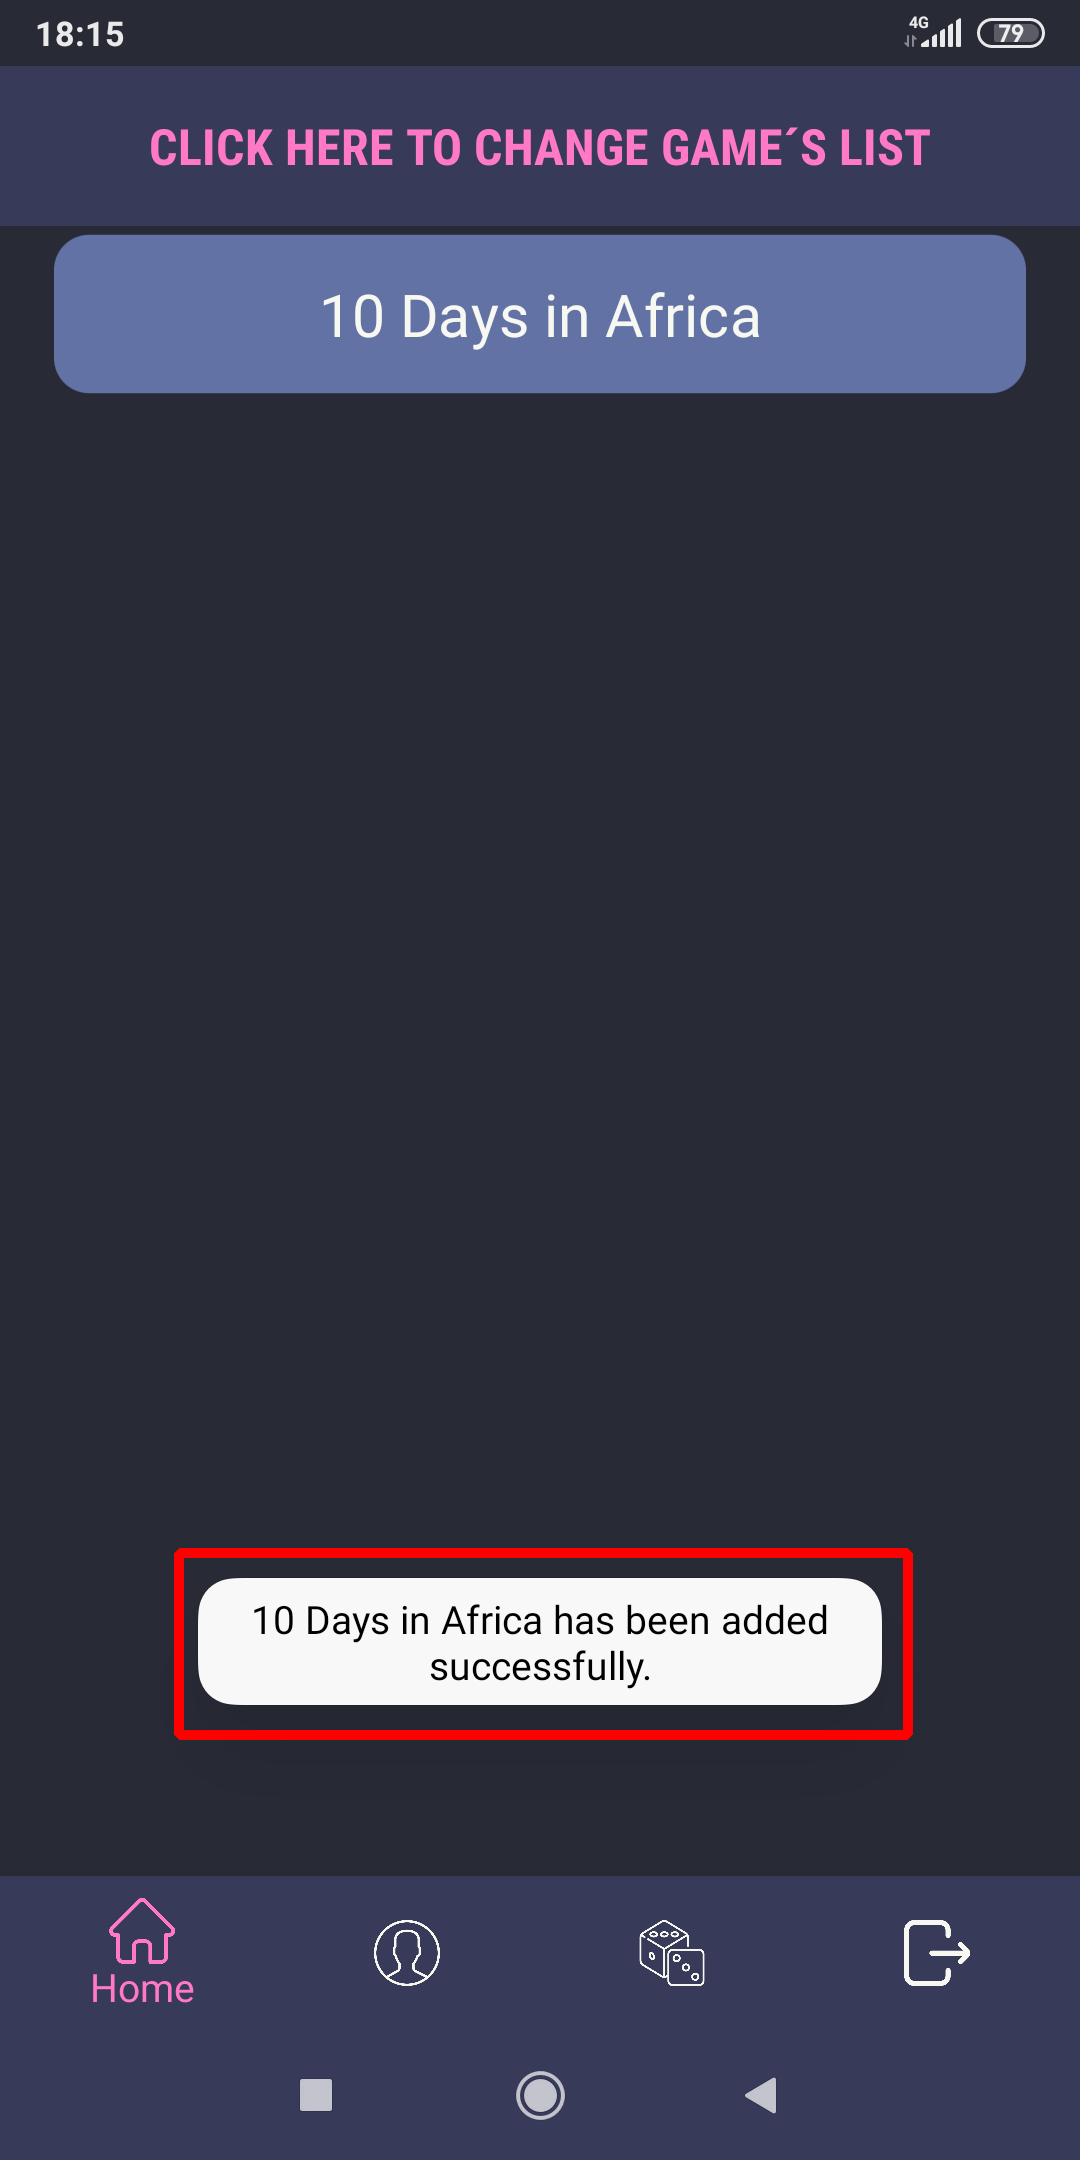
\includegraphics[width=0.3\linewidth]{fig/Uso/13.png}
    \caption{Notificación de que un juego ha sido añadido}
    \label{fig:uso13}
\end{figure}

Aclarar que la lista de juegos favoritos también tiene la capacidad de hacer scroll.

\begin{figure}[H]
    \centering
    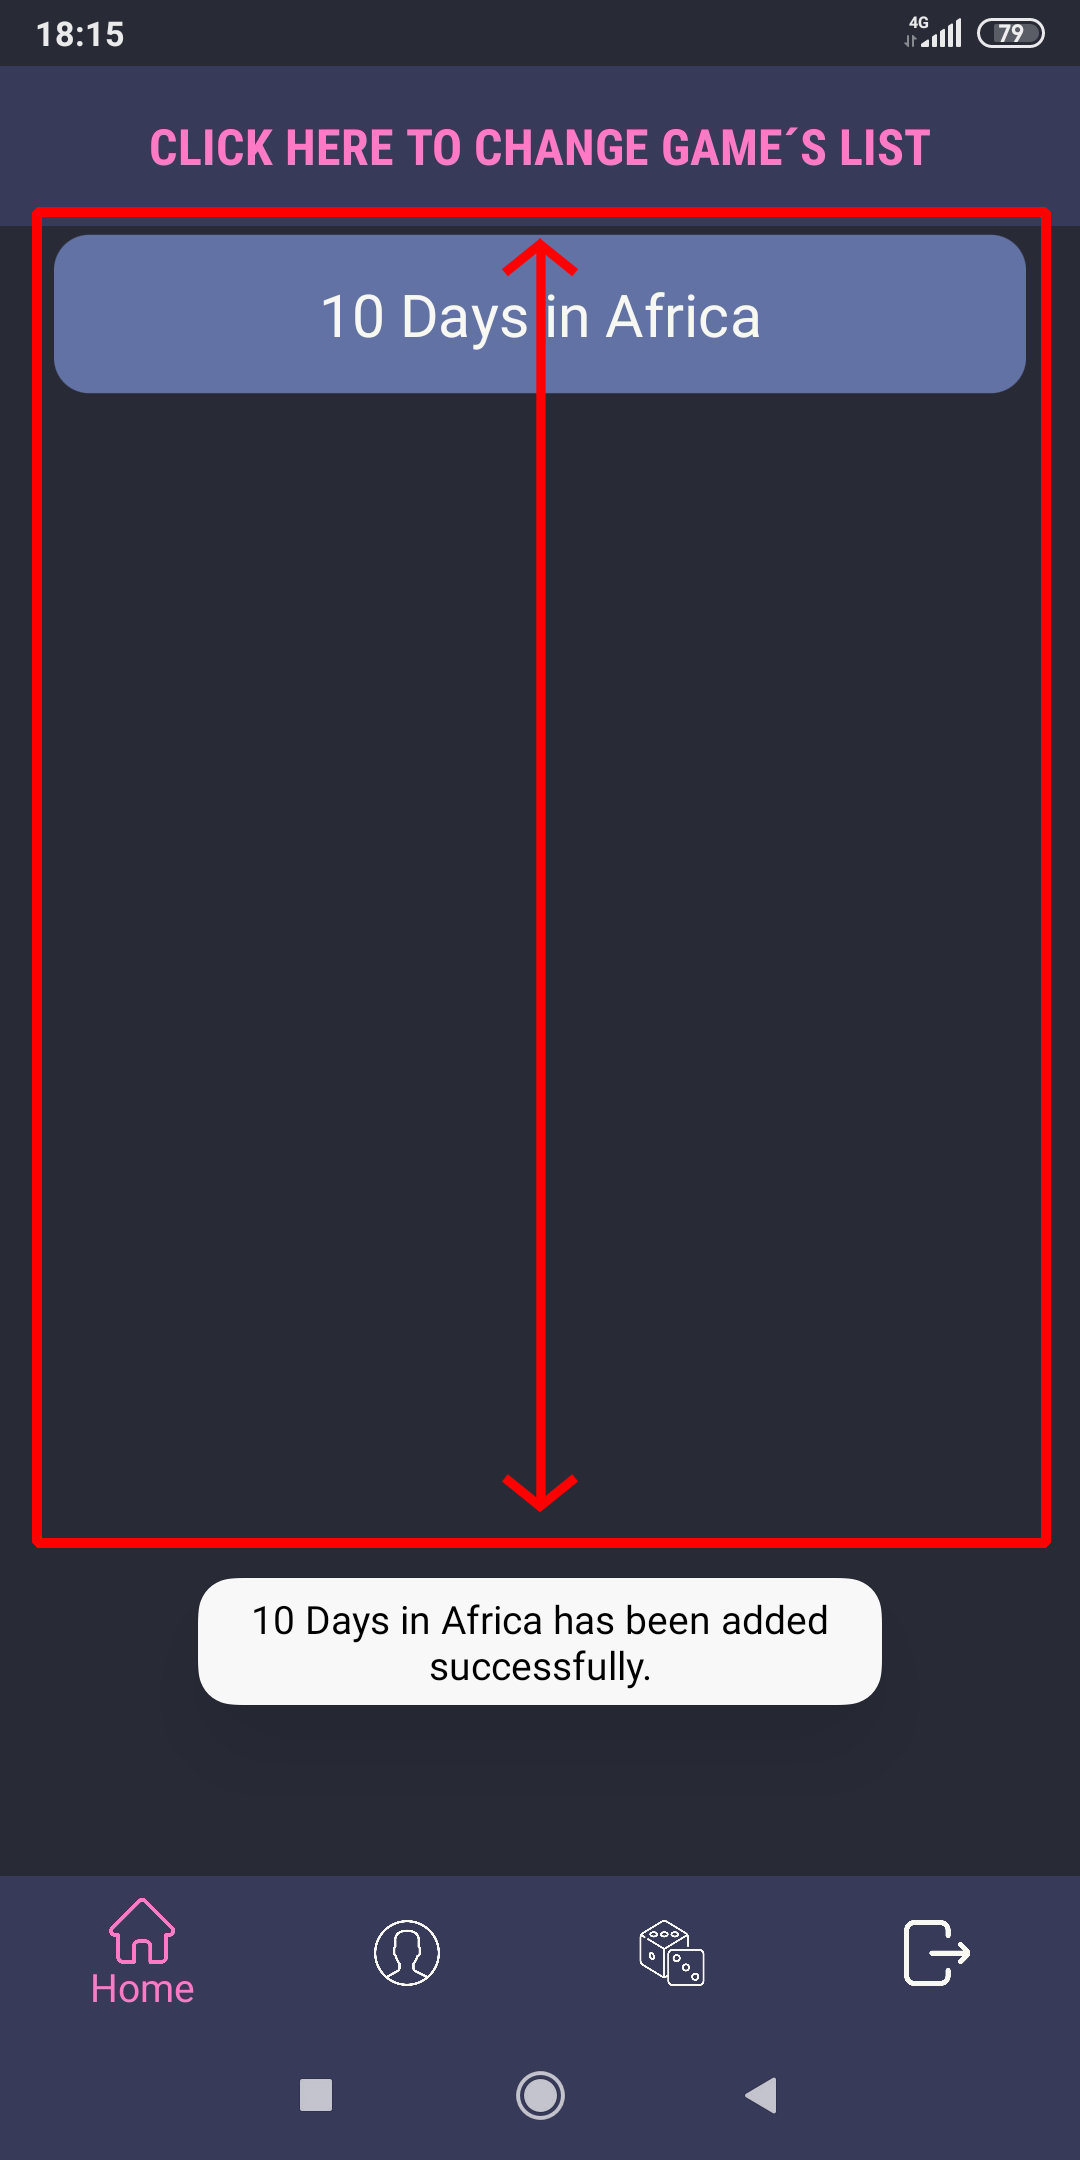
\includegraphics[width=0.3\linewidth]{fig/Uso/14.png}
    \caption{Scroll de lista de juegos favoritos}
    \label{fig:uso14}
\end{figure}

Cuando hacemos clic sobre uno de los juegos de esta lista, también nos abrirá una ventana con las estadísticas de este juego, pero con la diferencia de que ahora tendremos tres botones, en vez de uno único.

El primer botón que nos encontraremos será el que nos permita añadir partidas del juego seleccionado.

\begin{figure}[H]
    \centering
    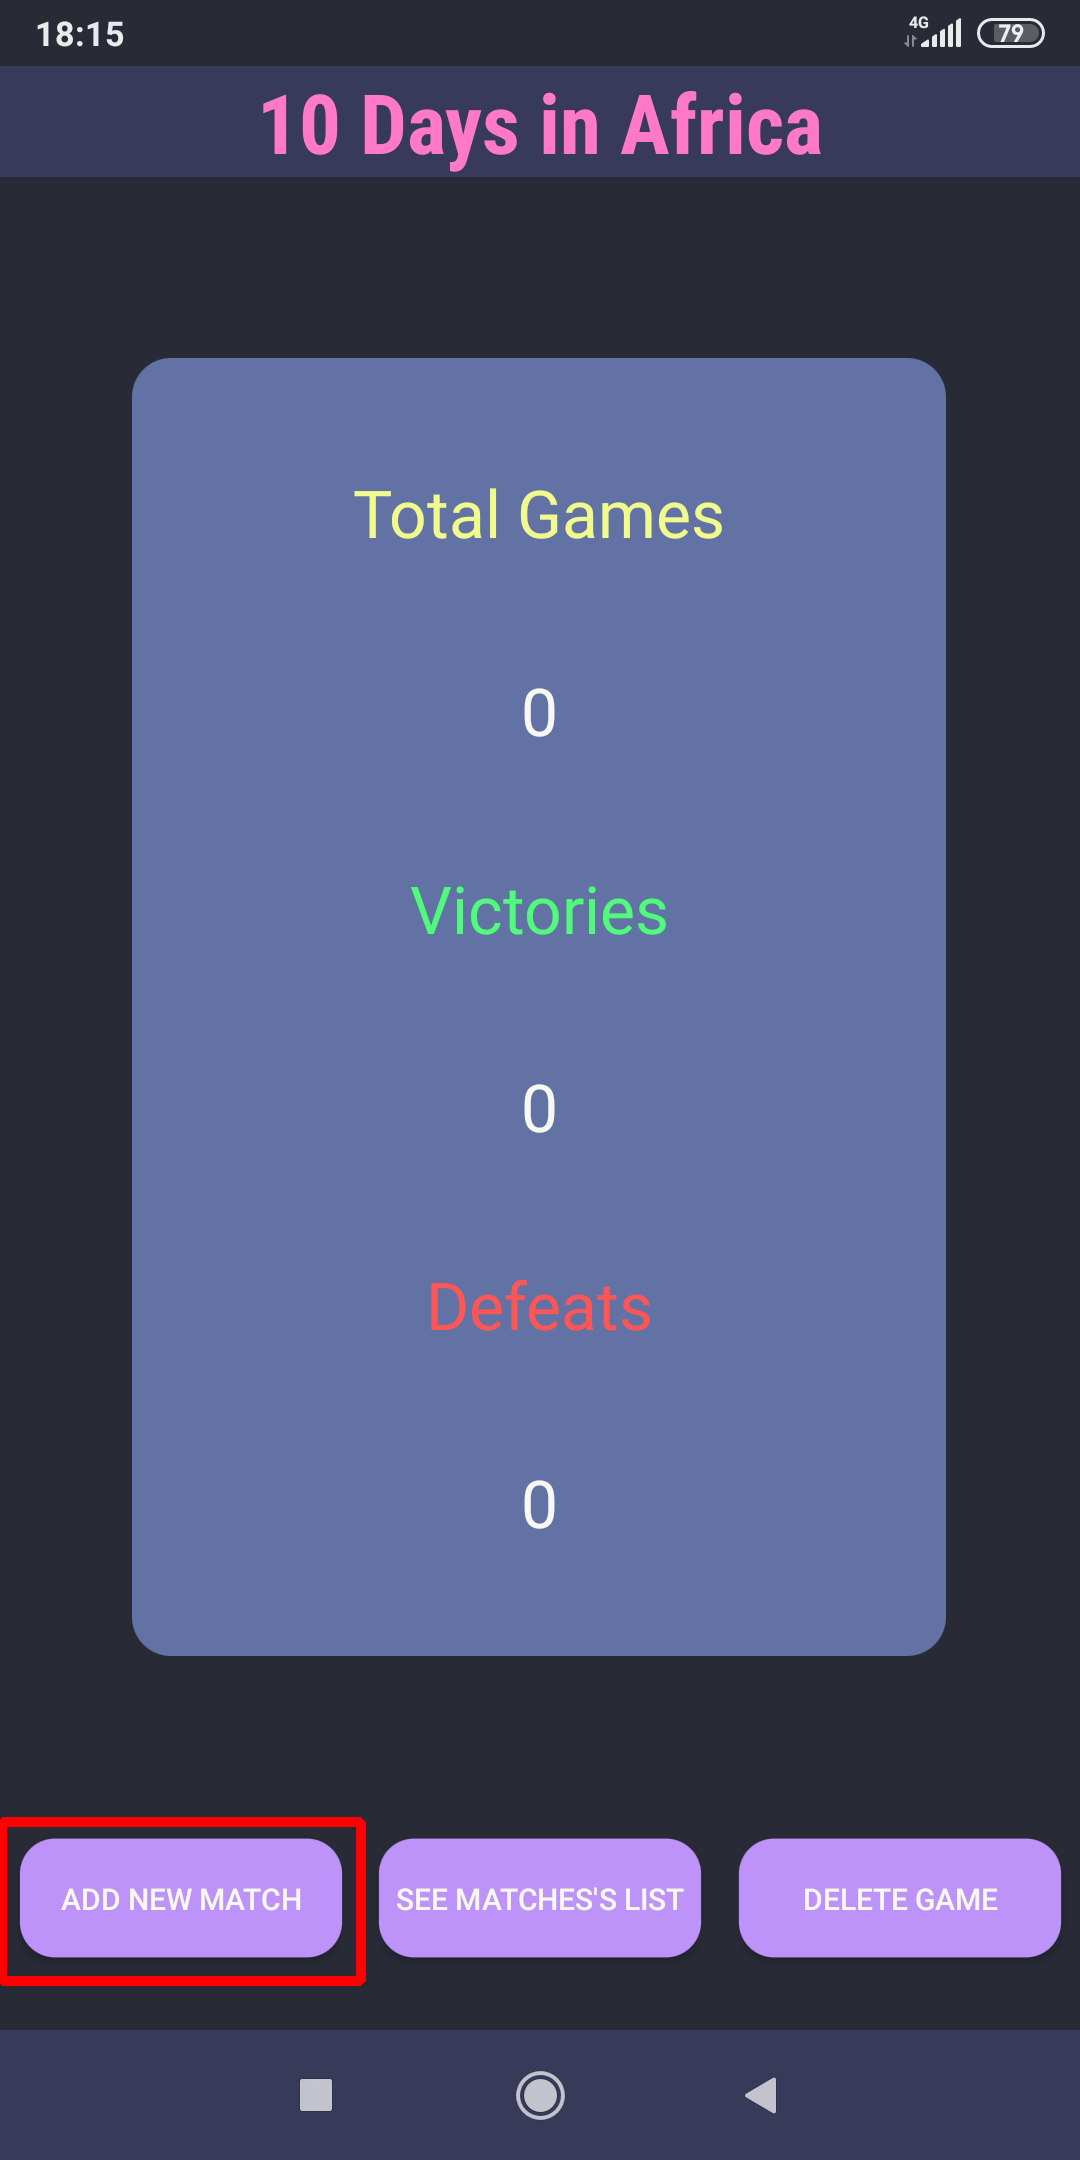
\includegraphics[width=0.3\linewidth]{fig/Uso/15.png}
    \caption{Botón para añadir partidas}
    \label{fig:uso15}
\end{figure}

Este botón nos abrirá la siguiente ventana en la que podremos escribir los nombres y las puntuaciones de hasta 8 jugadores.

Las puntuaciones serán añadidas a cada usuario y se le asignará una victoria o derrota dependiendo de su puntuación de forma automática.

\begin{figure}[H]
    \centering
    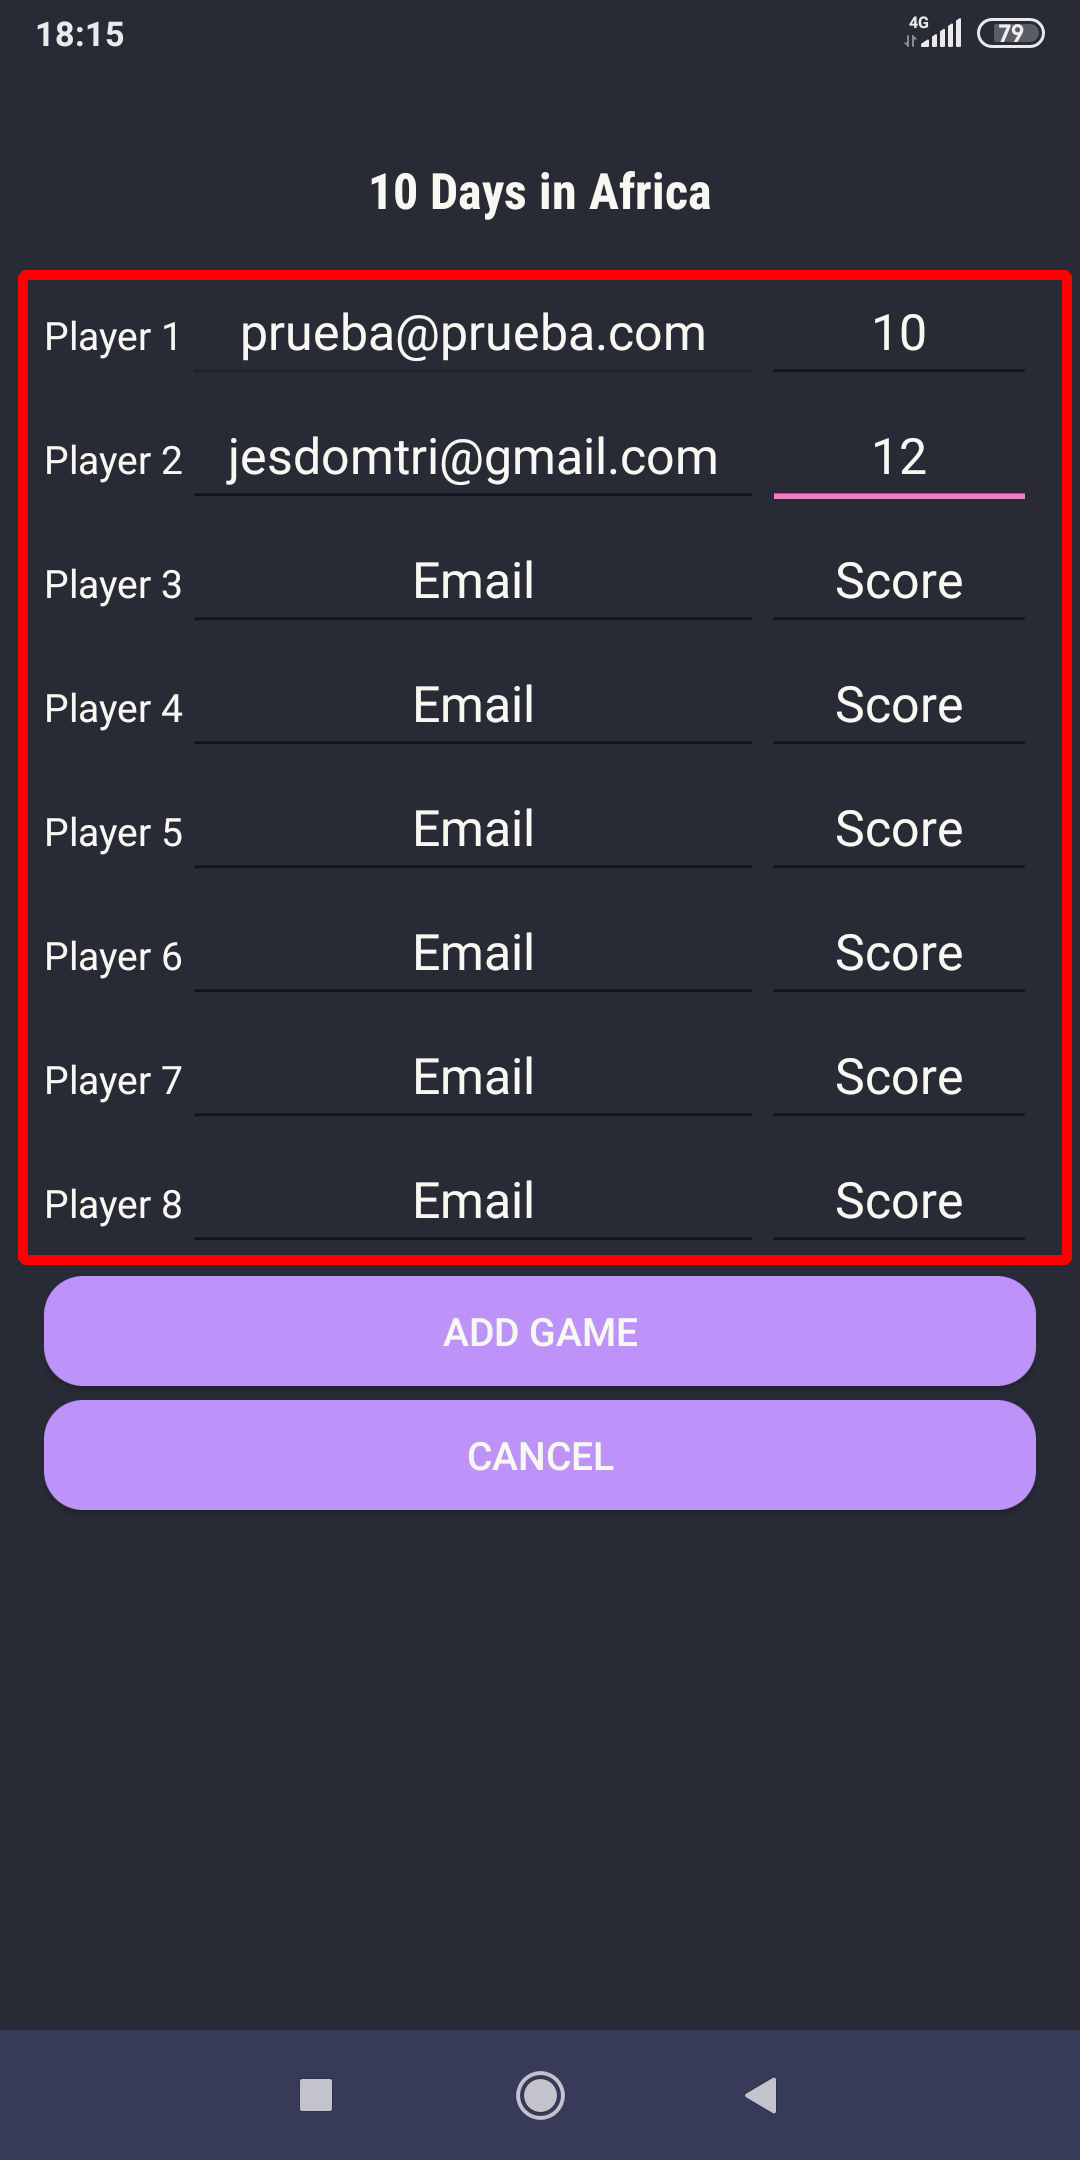
\includegraphics[width=0.3\linewidth]{fig/Uso/16.png}
    \caption{Añadir partida 1}
    \label{fig:uso16}
\end{figure}

\begin{figure}[H]
    \centering
    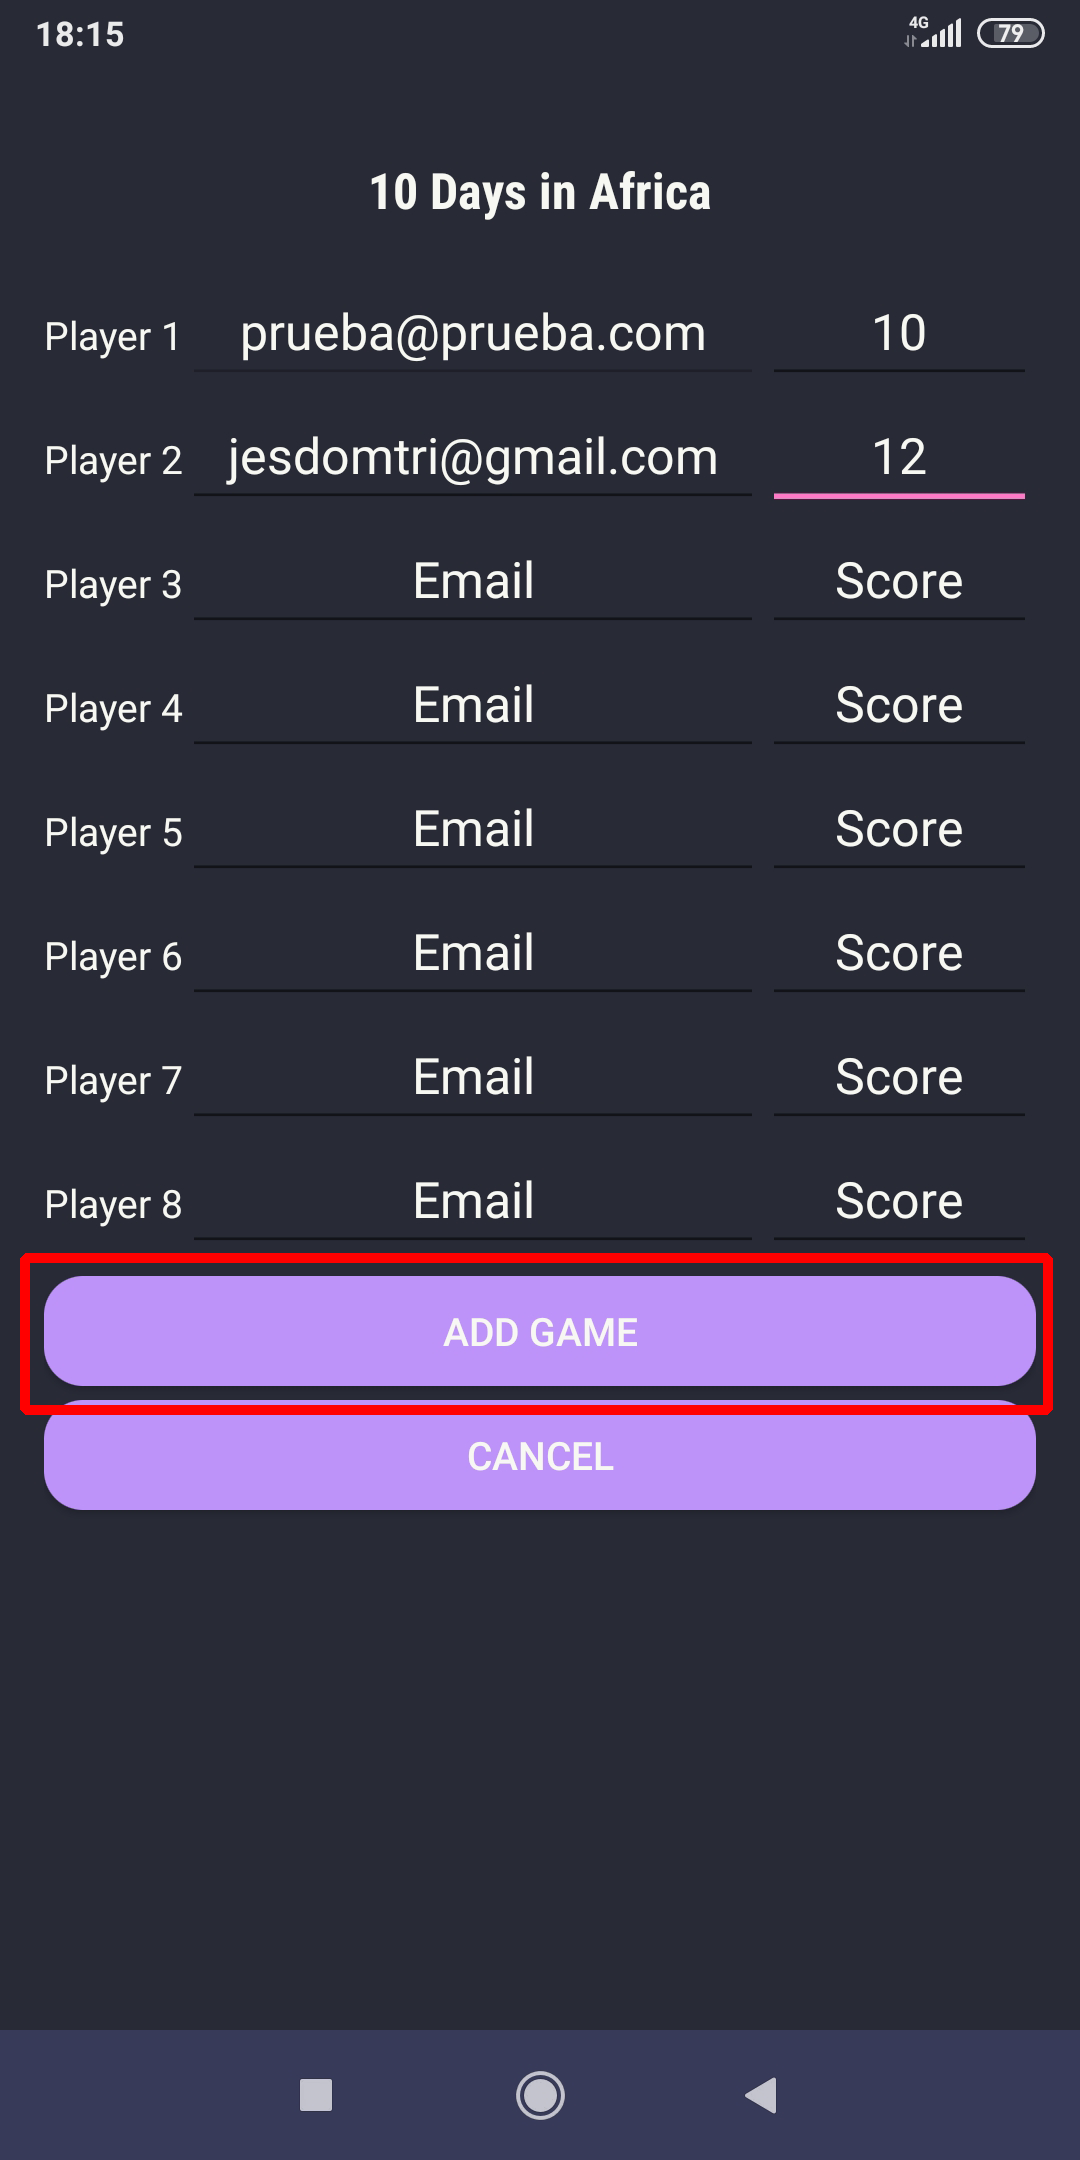
\includegraphics[width=0.3\linewidth]{fig/Uso/17.png}
    \caption{Añadir partida 2}
    \label{fig:uso17}
\end{figure}

Registrando dos partidas nos quedará algo como lo siguiente.

\begin{figure}[H]
    \centering
    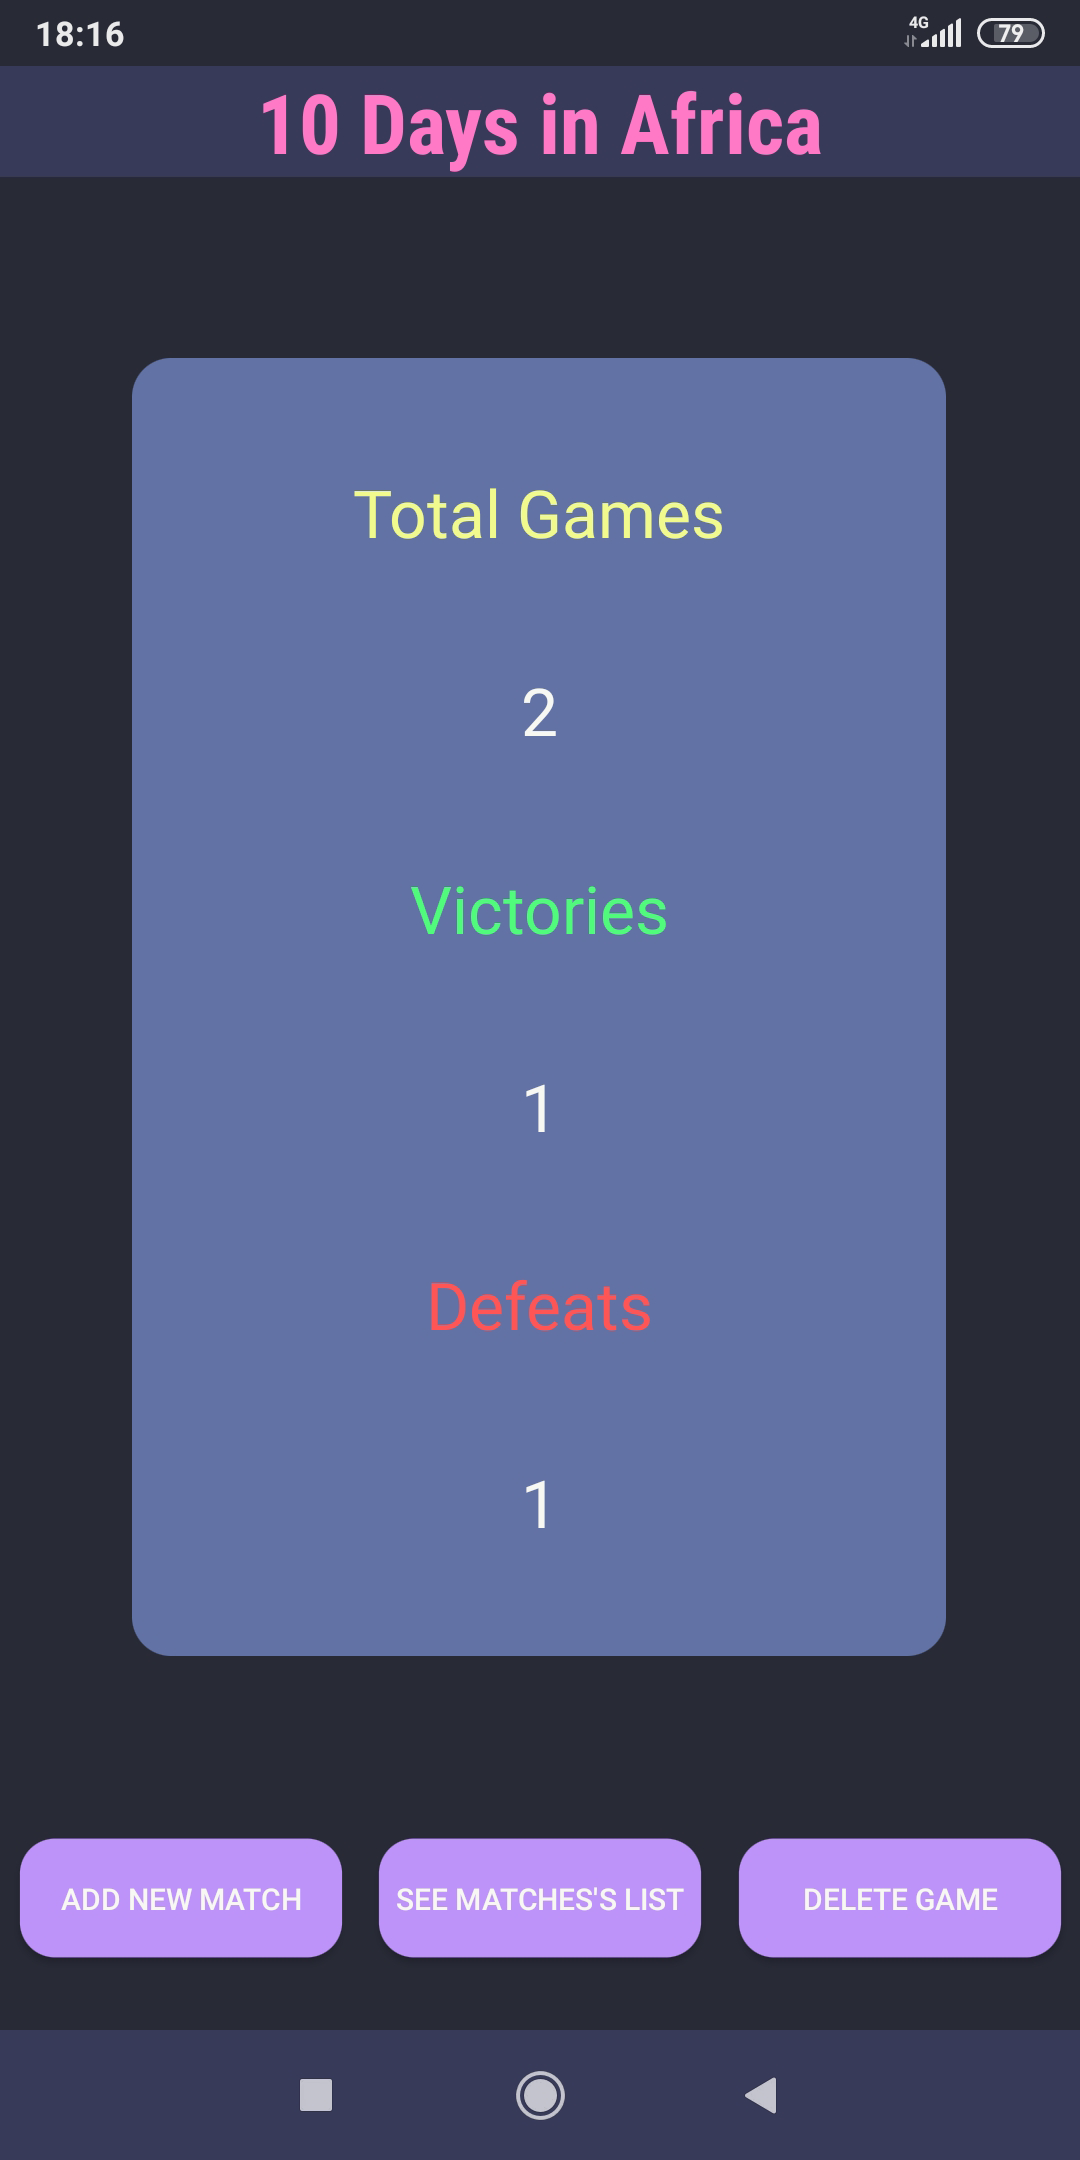
\includegraphics[width=0.3\linewidth]{fig/Uso/18.png}
    \caption{Partidas añadidas}
    \label{fig:uso18}
\end{figure}

Pulsando el botón para ver la lista de partidas de ese juego

\begin{figure}[H]
    \centering
    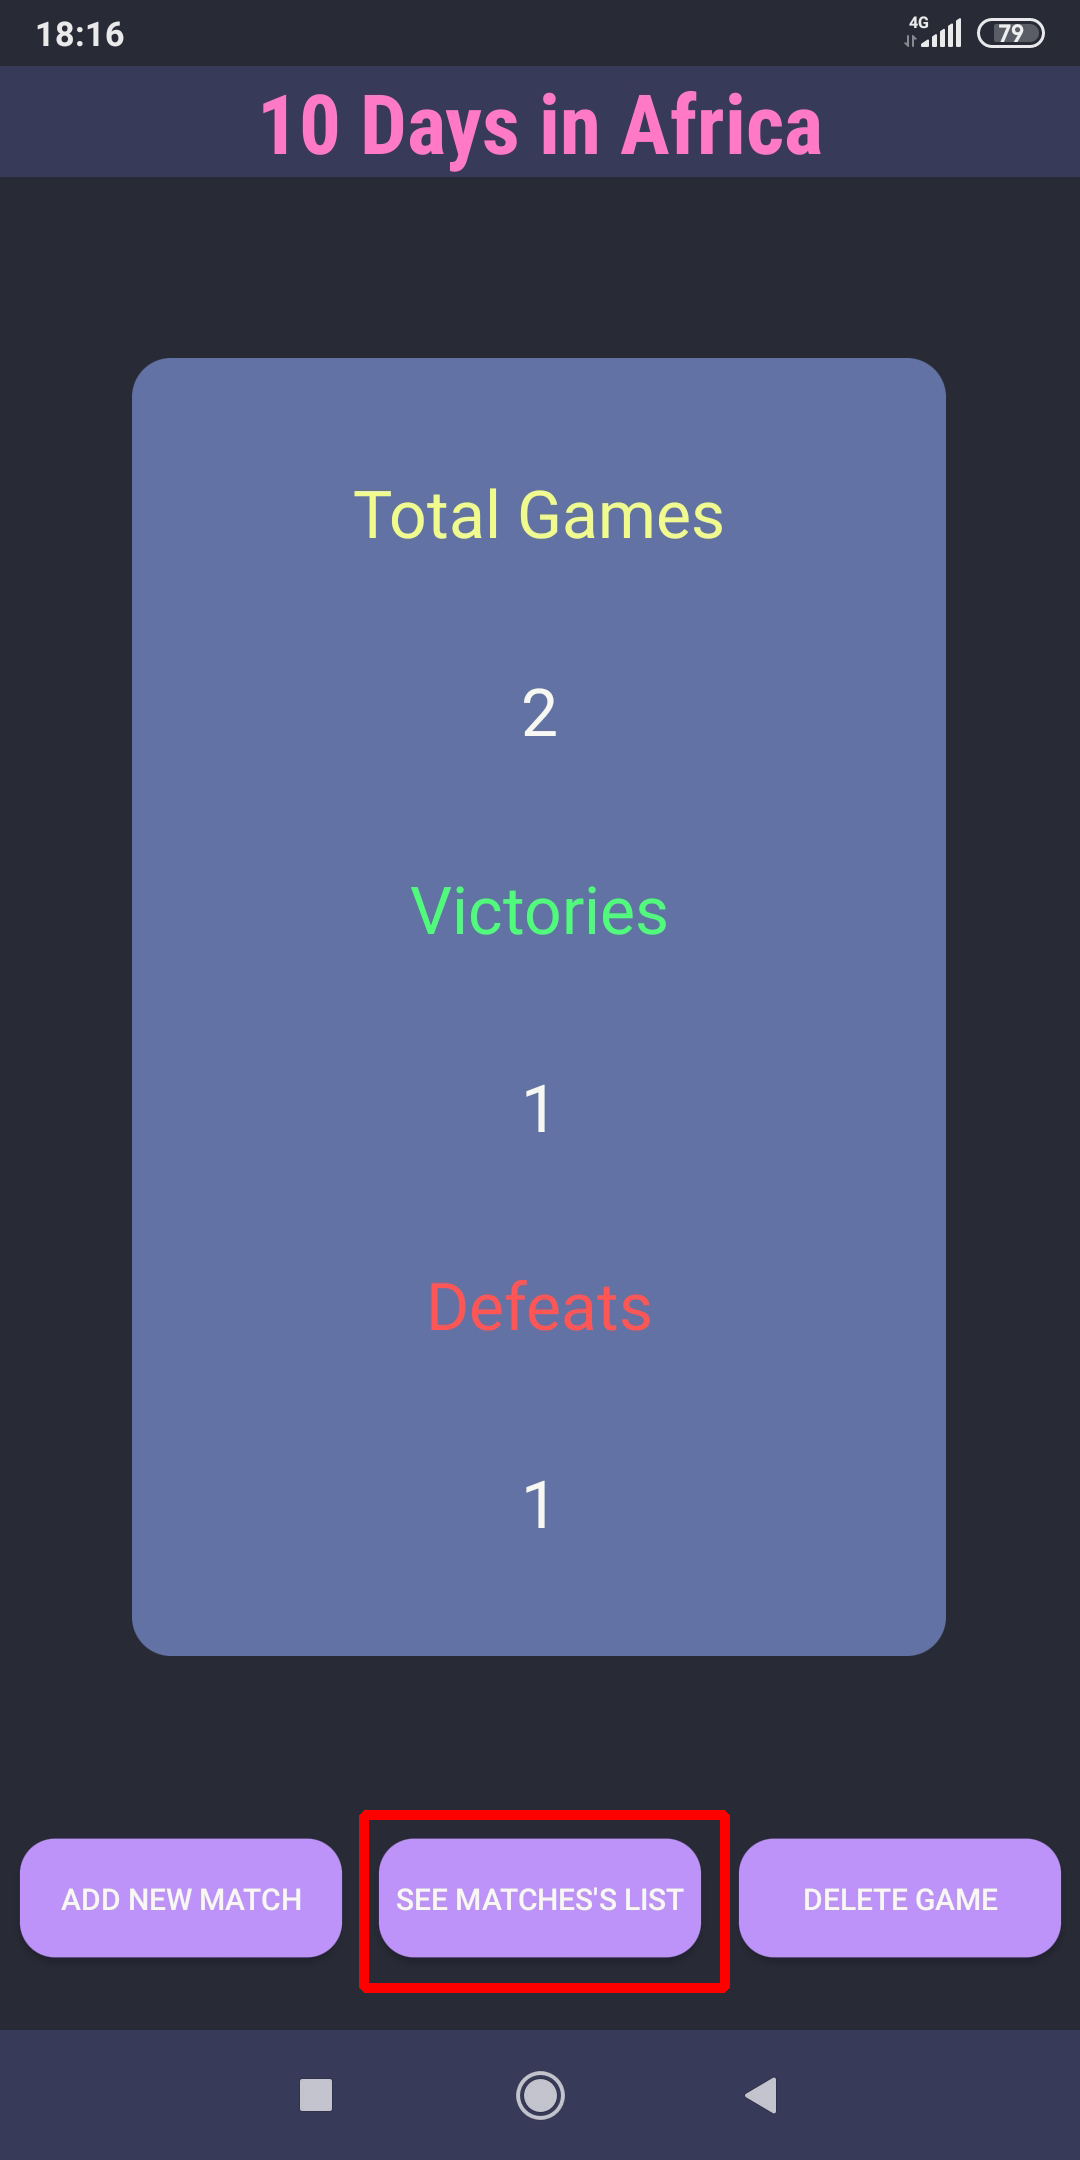
\includegraphics[width=0.3\linewidth]{fig/Uso/19.png}
    \caption{Botón de lista de partidas}
    \label{fig:uso19}
\end{figure}

nos mostrará la siguiente ventana con una lista de partidas reflejando nuestra puntuación, posición y una corona que solamente se mostrará en las partidas que hayamos acabado en primera posición.

\begin{figure}[H]
    \centering
    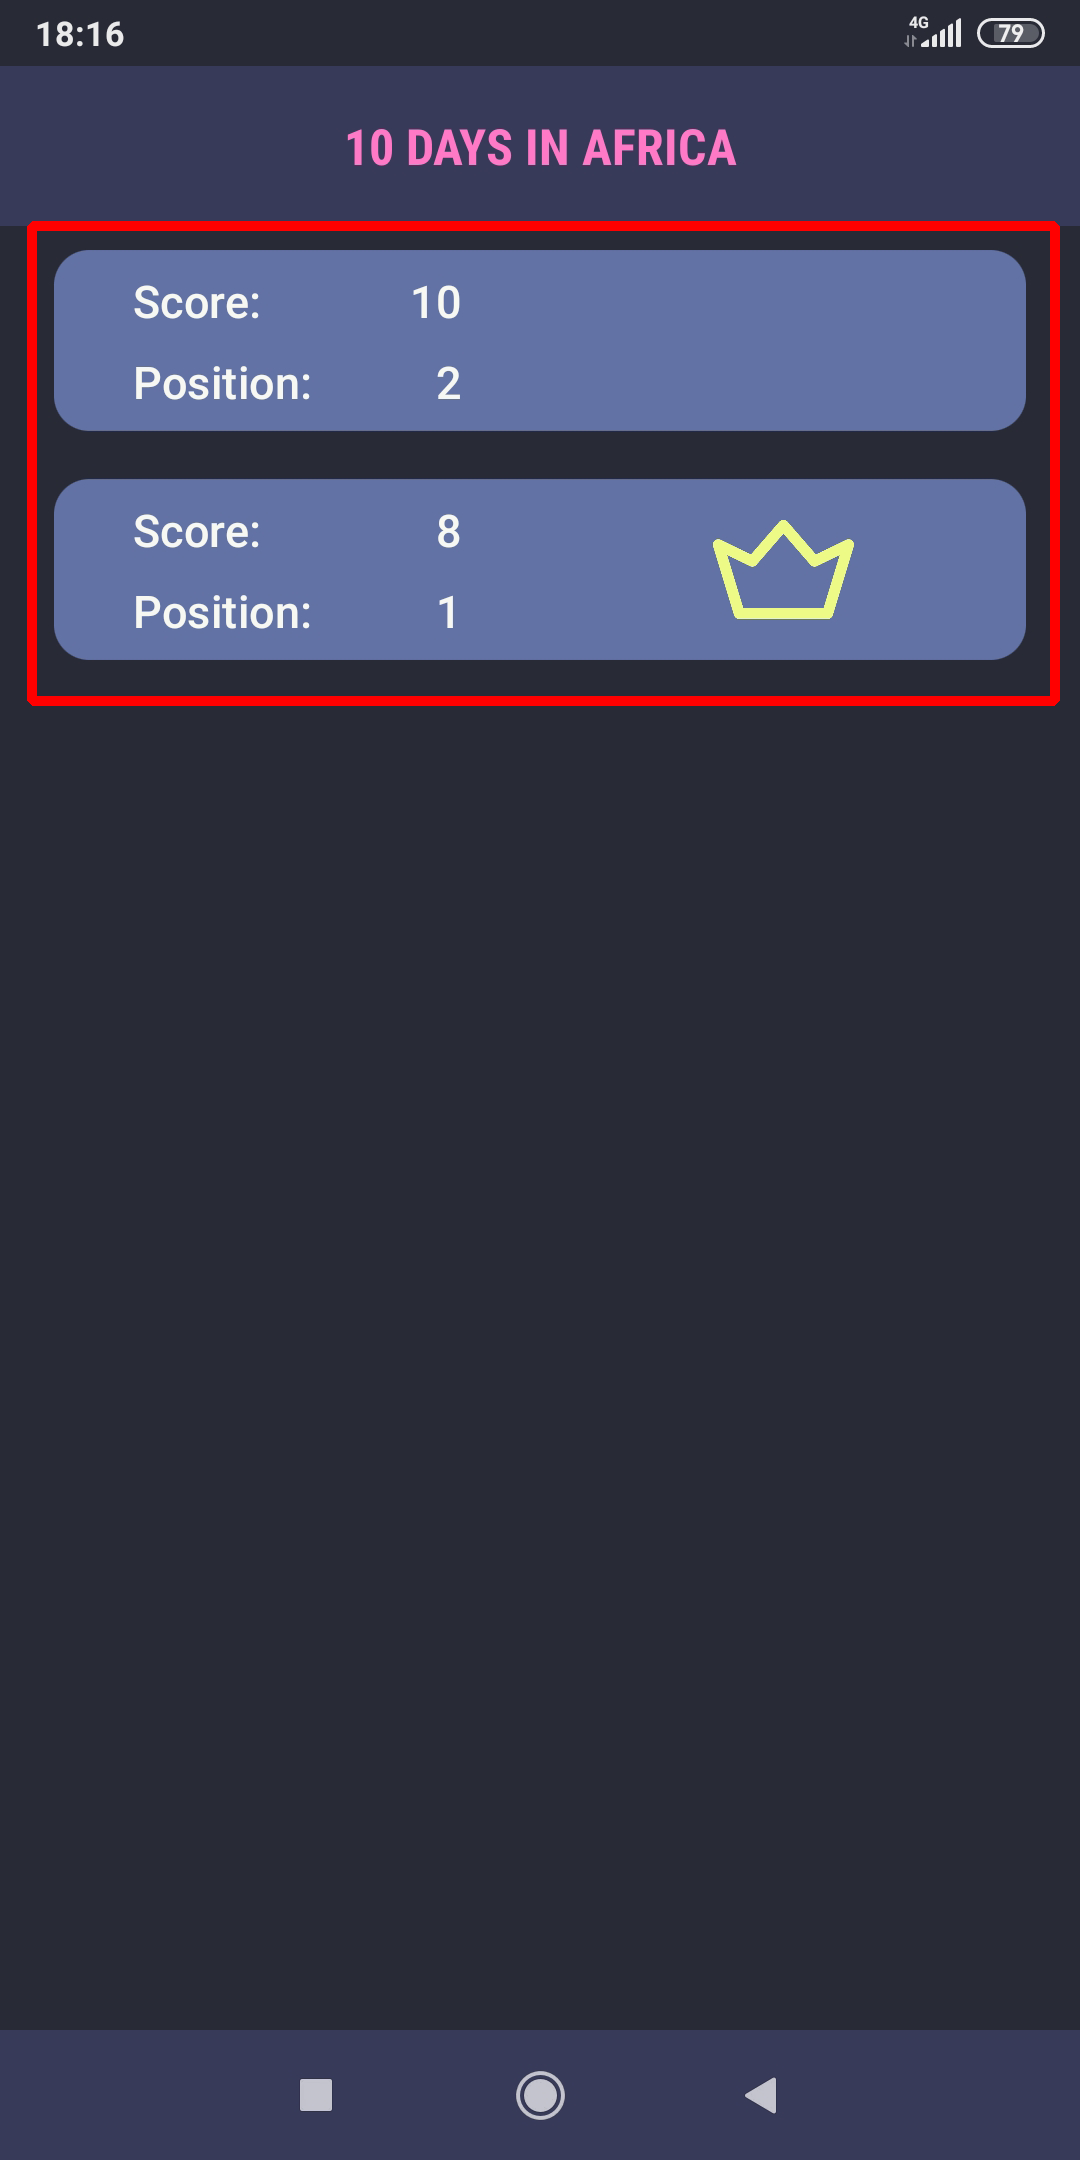
\includegraphics[width=0.3\linewidth]{fig/Uso/20.png}
    \caption{Lista de partidas}
    \label{fig:uso20}
\end{figure}

Por último, pulsando el tercer botón, borraremos este juego de la lista de juegos favoritos, cuya acción también nos será notificada como cuando añadimos un juego, mediante un mensaje al usuario en pantalla.

\begin{figure}[H]
    \centering
    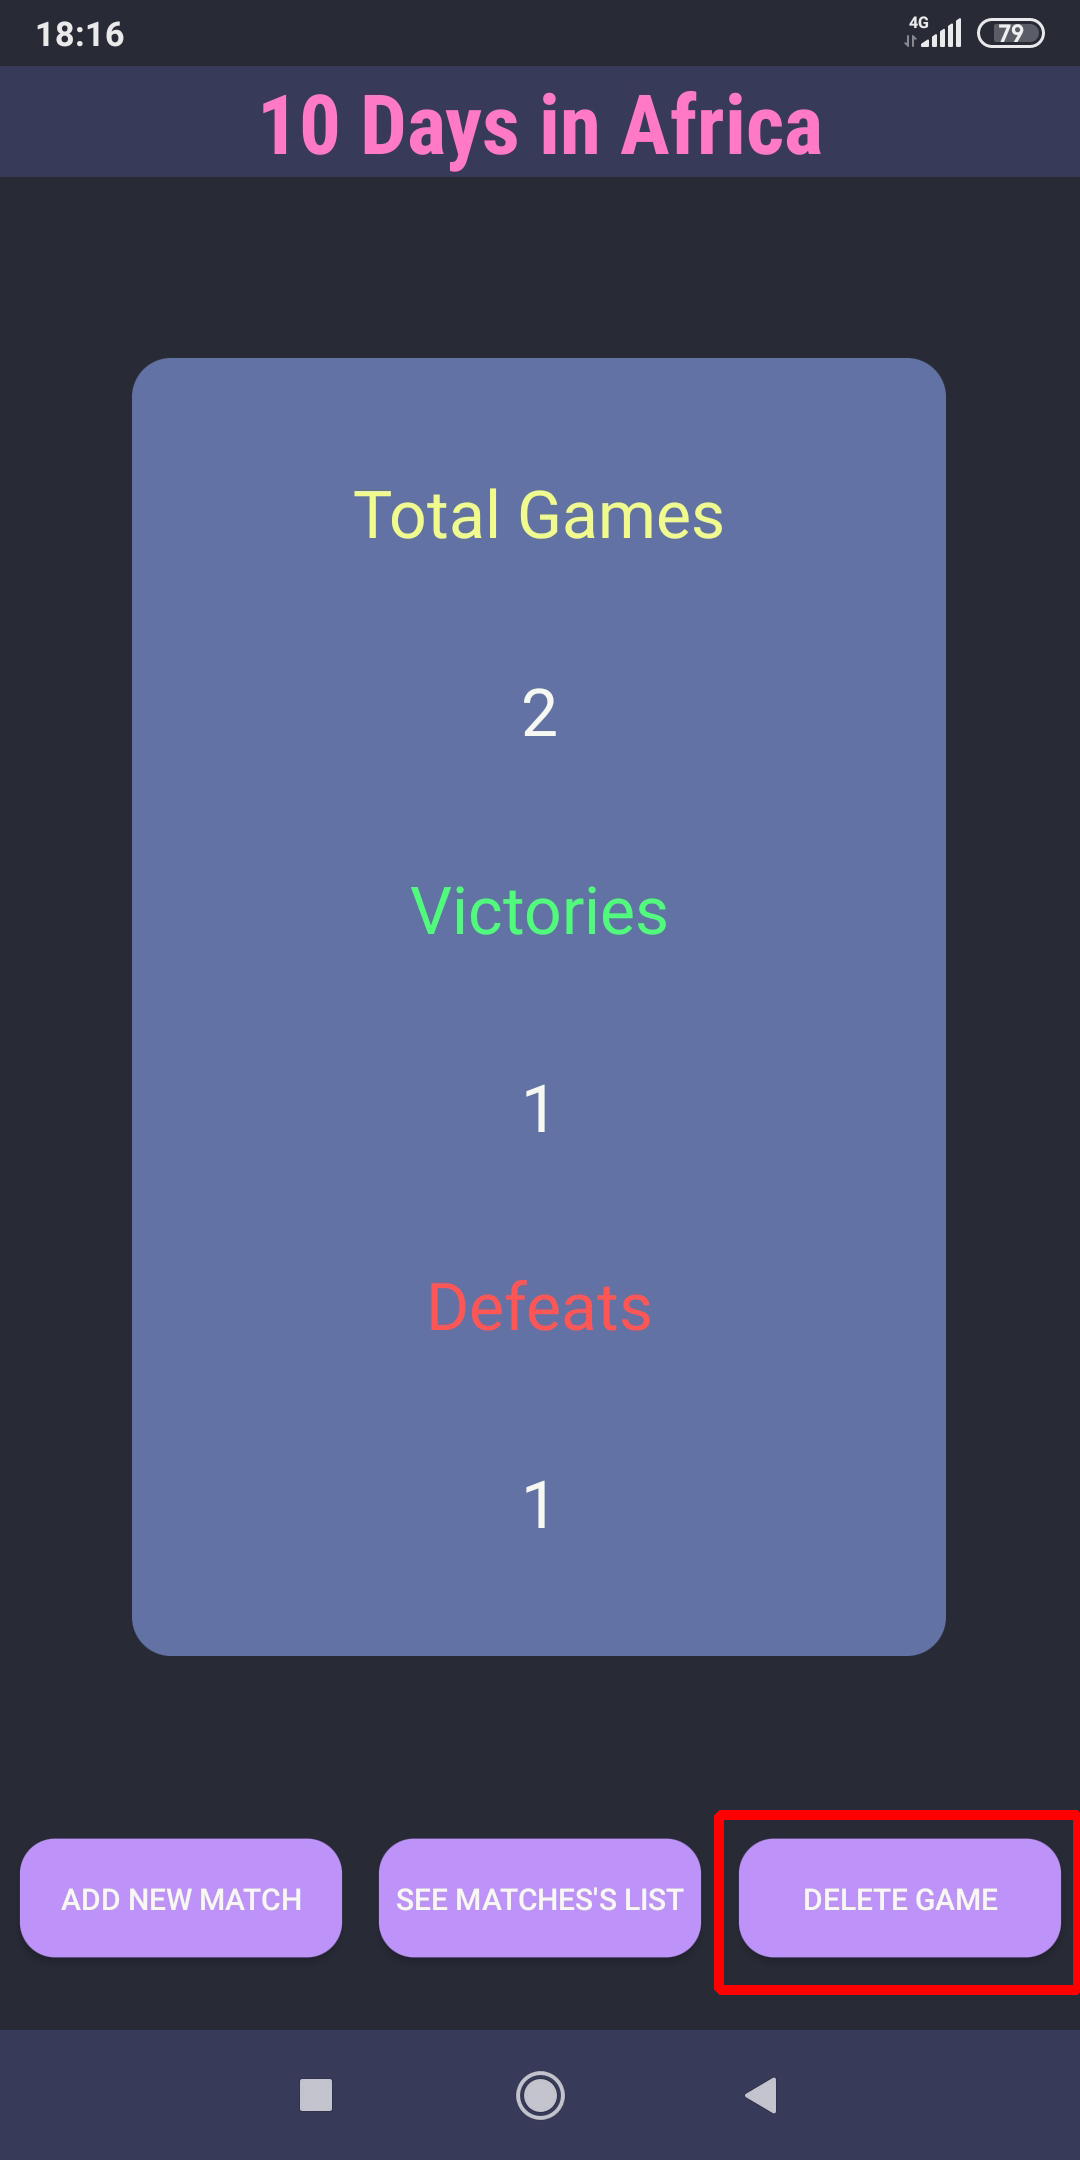
\includegraphics[width=0.3\linewidth]{fig/Uso/21.png}
    \caption{Borrar juego favorito 1}
    \label{fig:uso21}
\end{figure}

\begin{figure}[H]
    \centering
    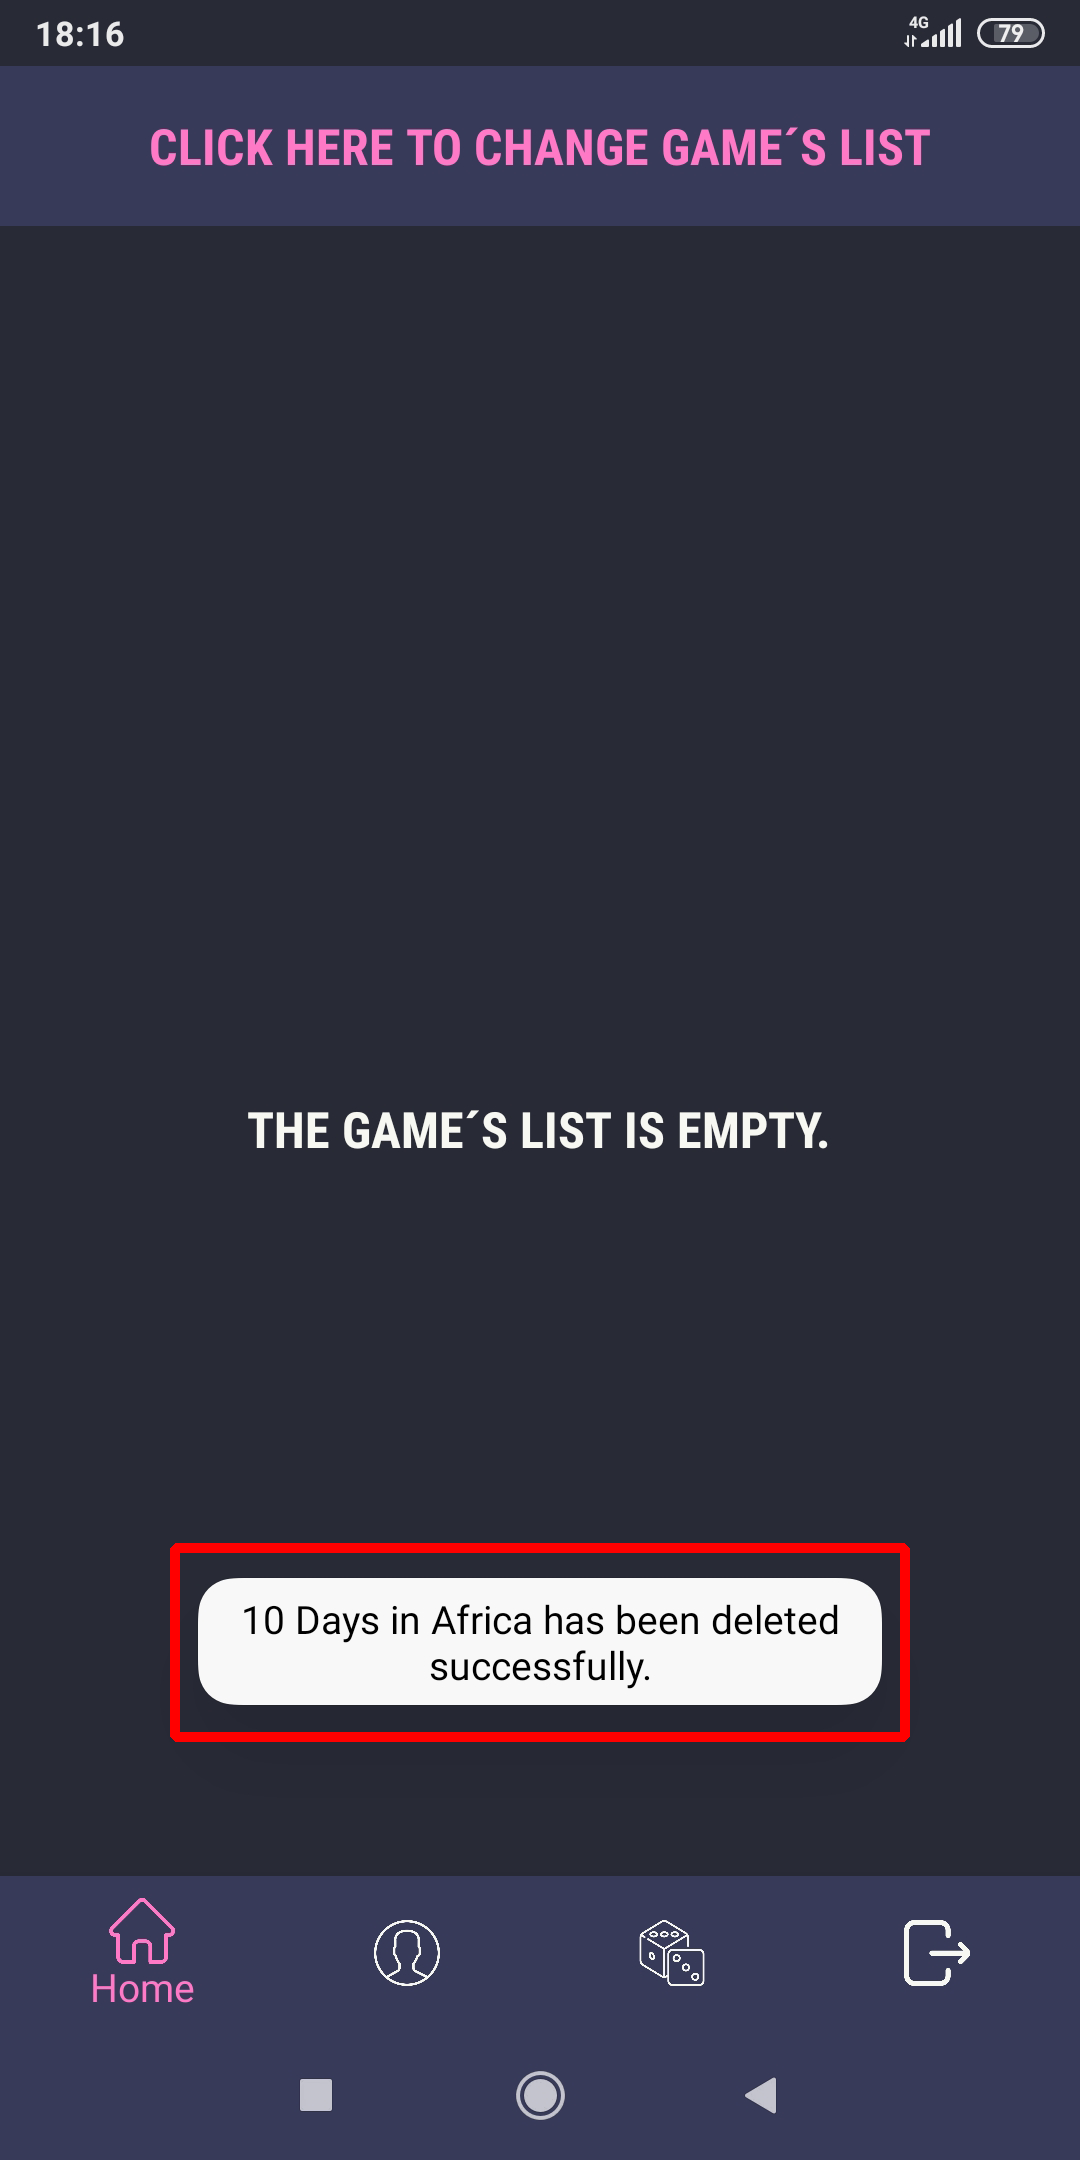
\includegraphics[width=0.3\linewidth]{fig/Uso/22.png}
    \caption{Borrar juego favorito 2}
    \label{fig:uso22}
\end{figure}

Desde la segunda ventana que nos abrirá la barra de navegación podremos ver nuestros datos de usuario. En específico, nuestro correo electrónico, contraseña modificada con asteriscos, un botón para restablecer esta última, nuestro identificador de usuario y la fecha en la que nos registramos.

\begin{figure}[H]
    \centering
    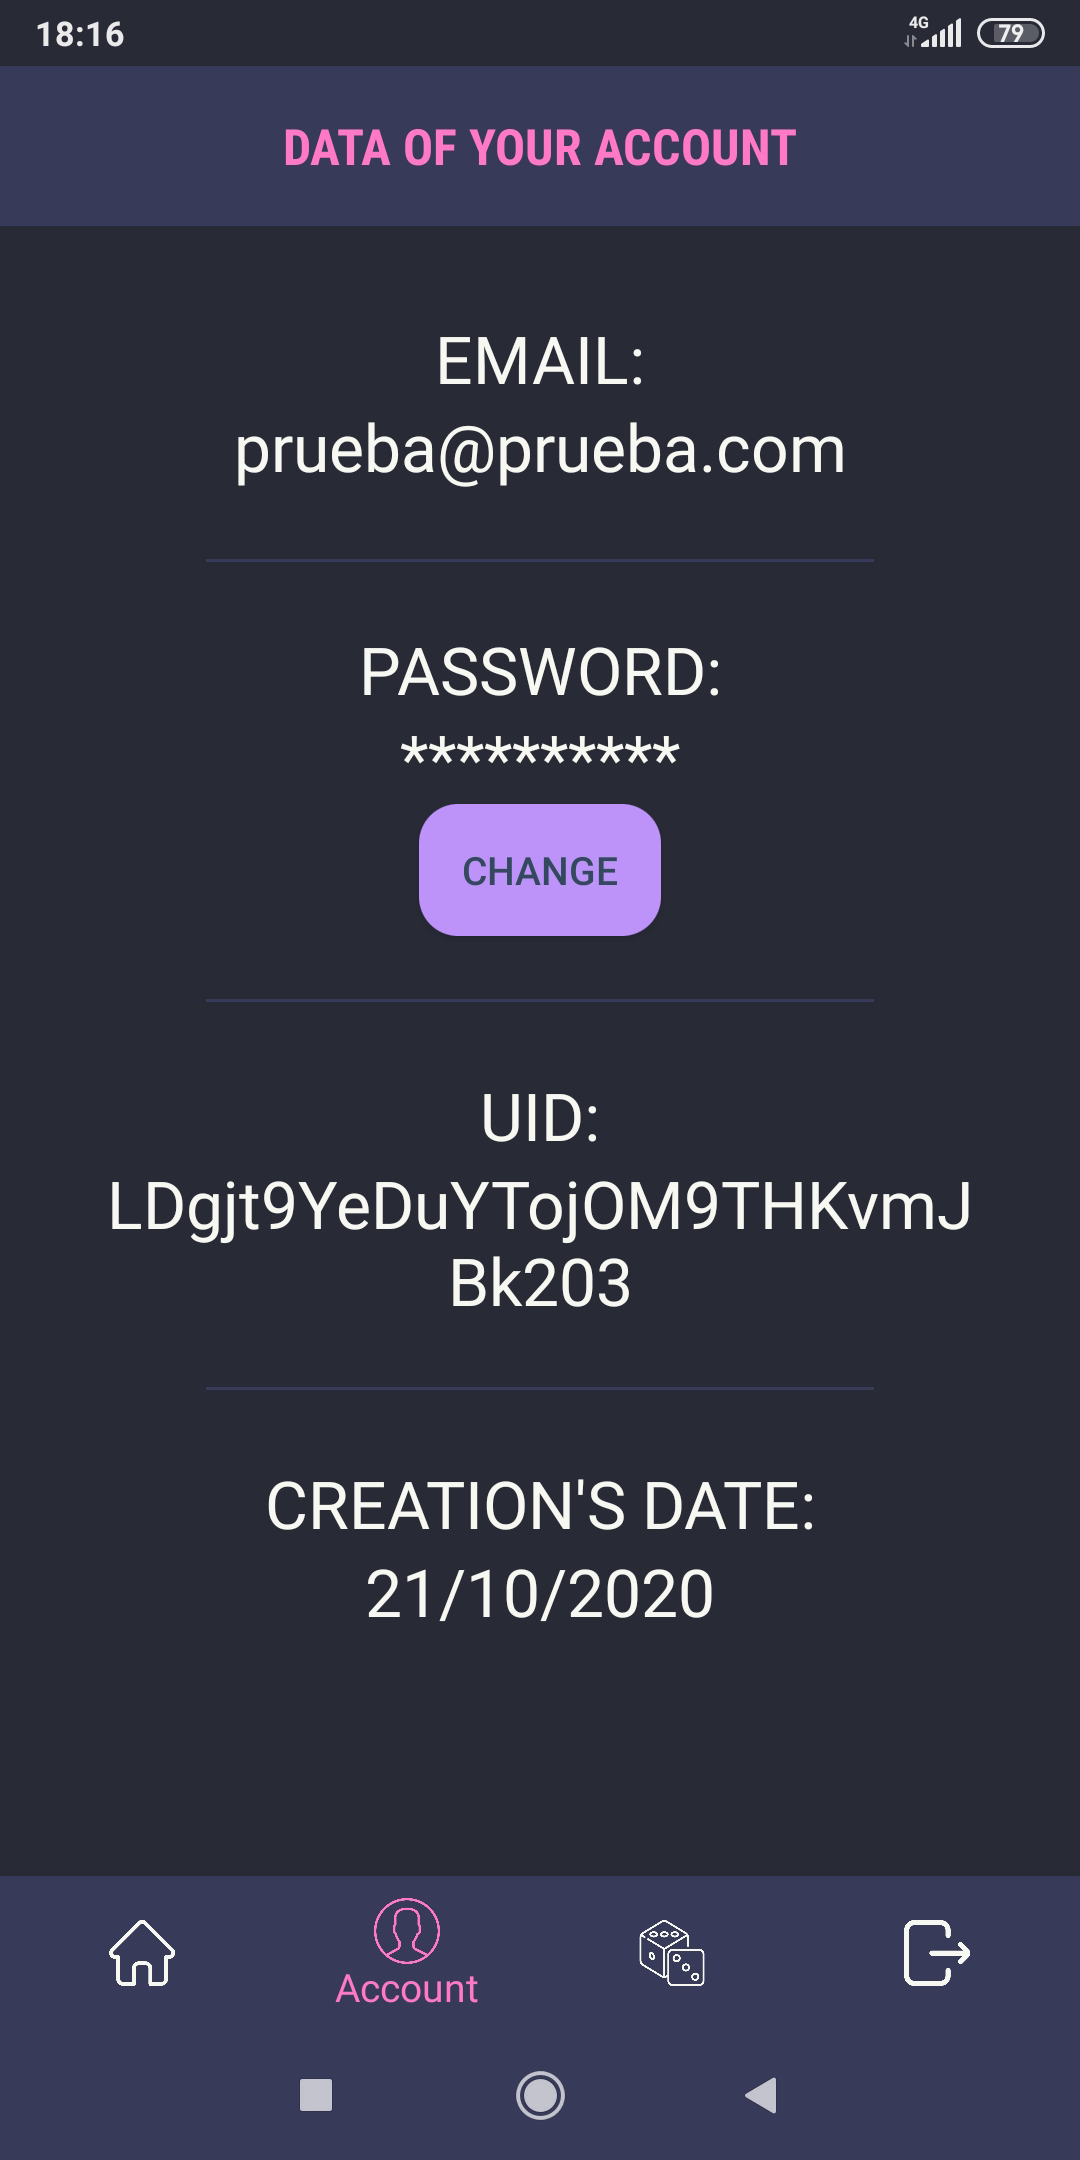
\includegraphics[width=0.3\linewidth]{fig/Uso/23.png}
    \caption{Datos de usuario 1}
    \label{fig:uso23}
\end{figure}

\begin{figure}[H]
    \centering
    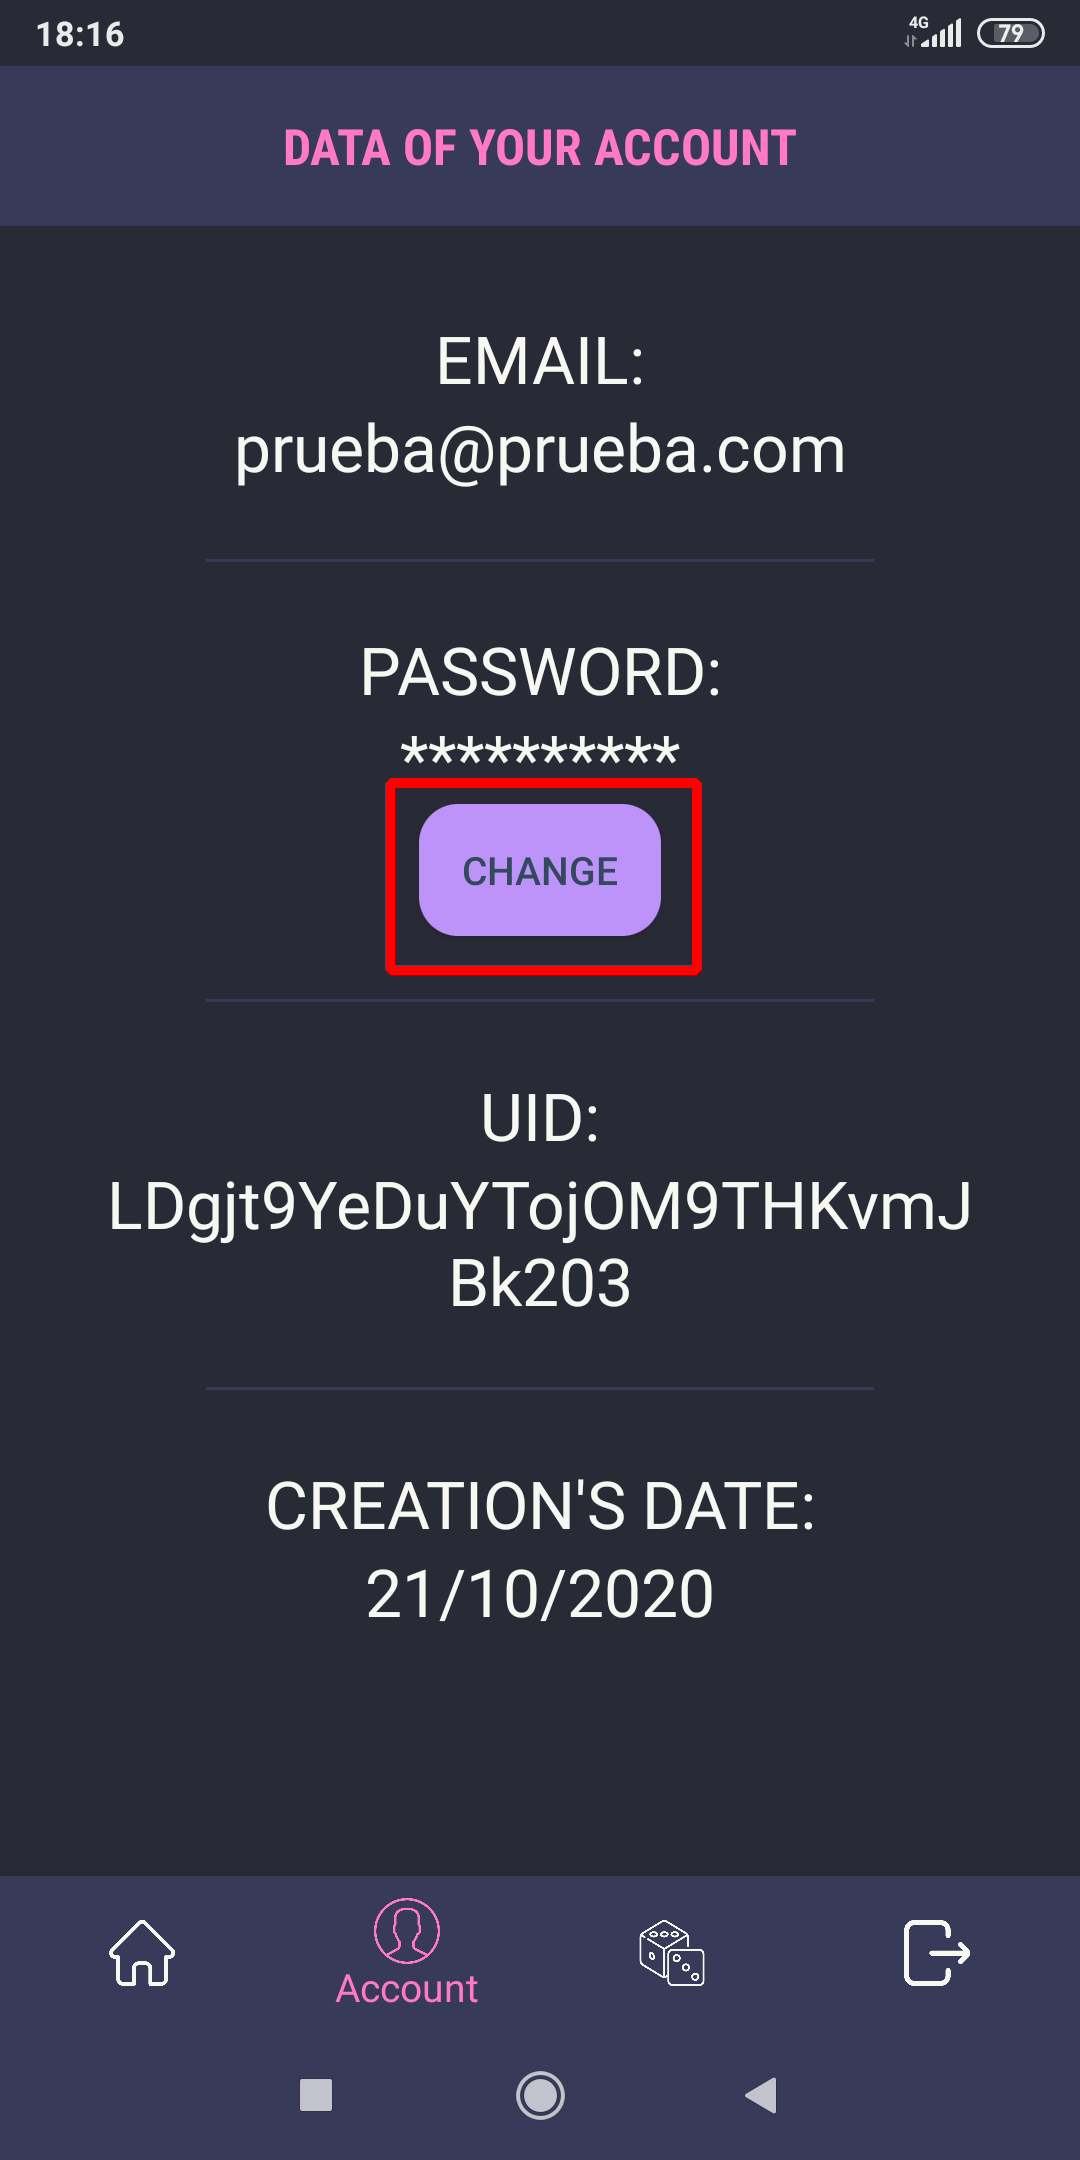
\includegraphics[width=0.3\linewidth]{fig/Uso/24.png}
    \caption{Datos de usuario 2}
    \label{fig:uso24}
\end{figure}

\begin{figure}[H]
    \centering
    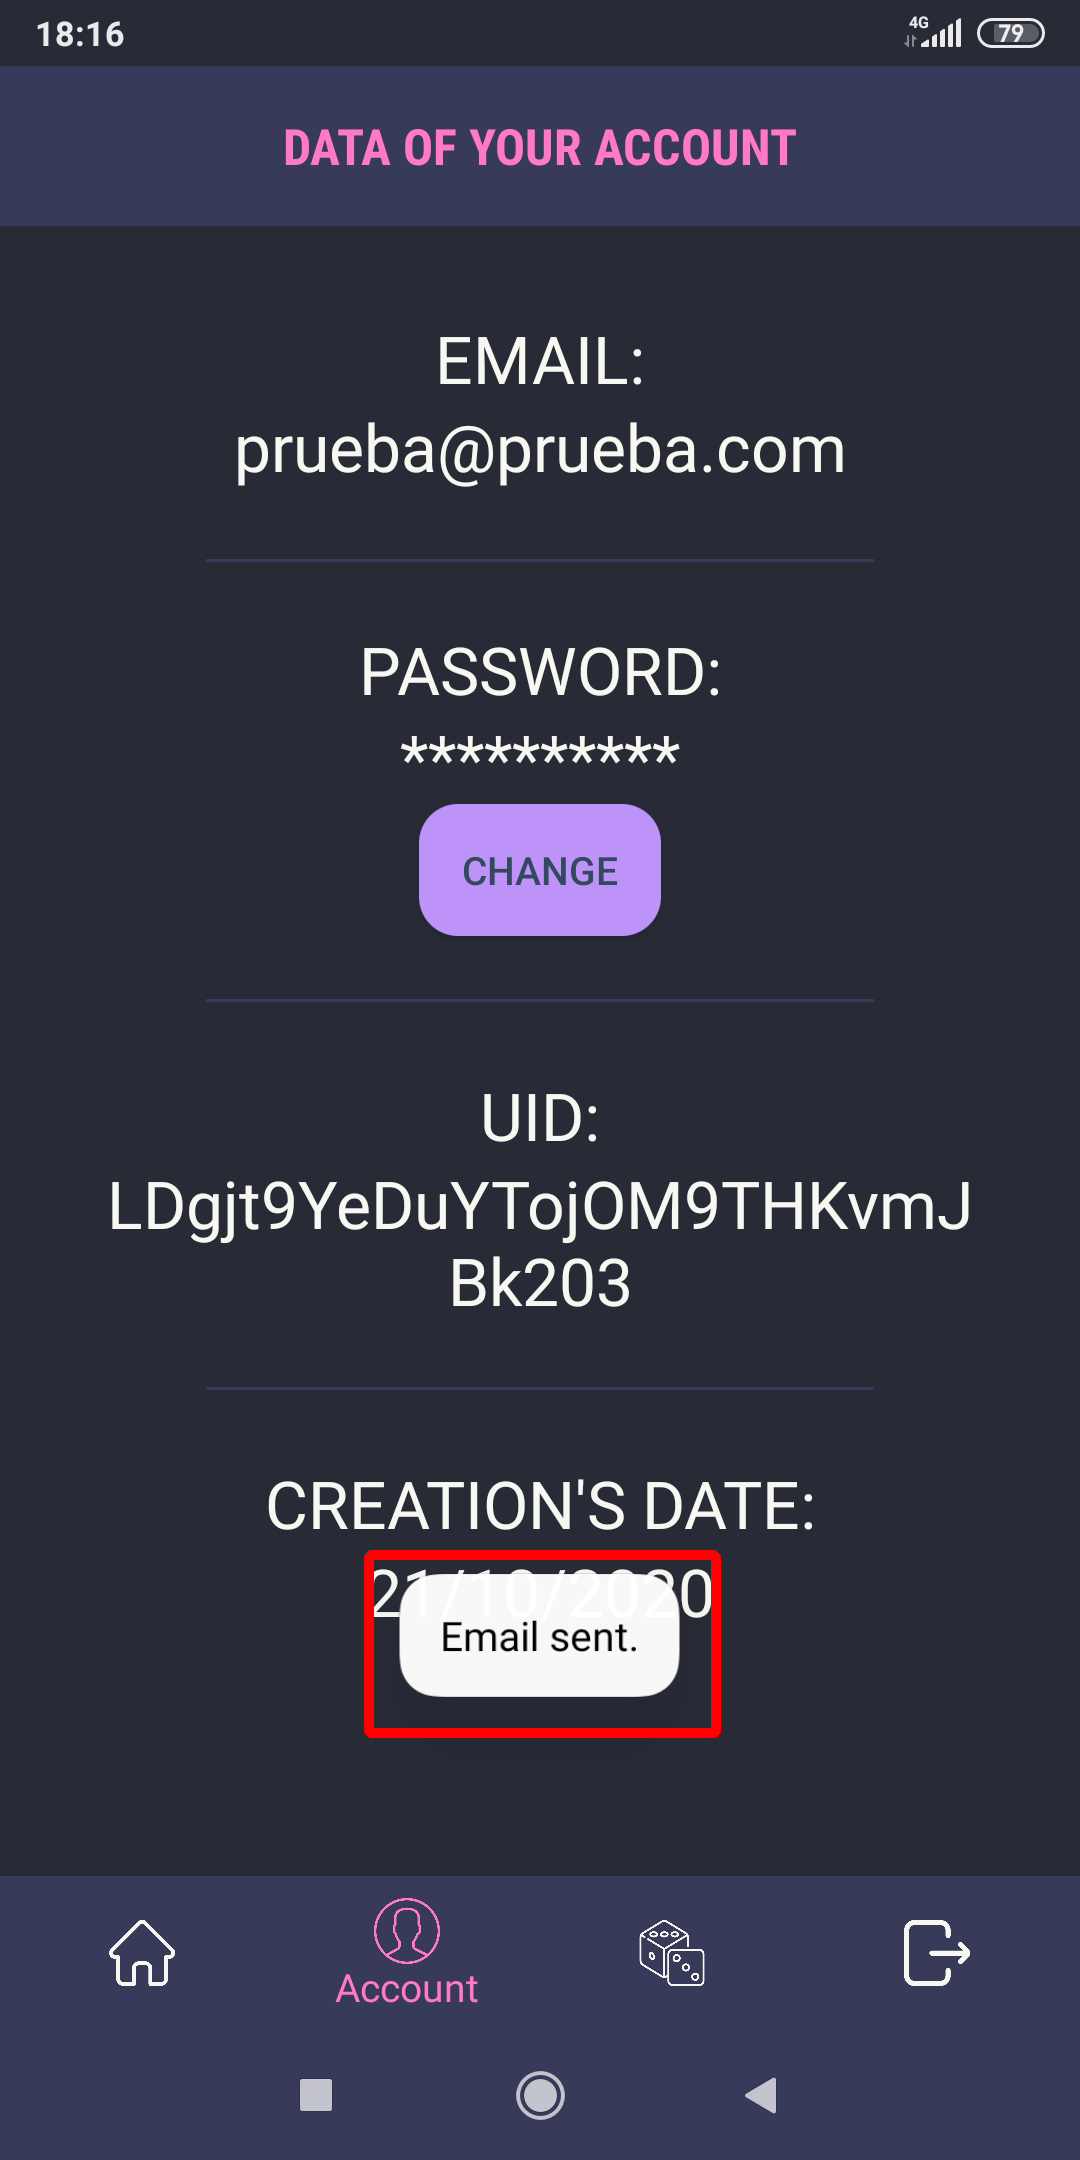
\includegraphics[width=0.3\linewidth]{fig/Uso/25.png}
    \caption{Datos de usuario 3}
    \label{fig:uso25}
\end{figure}

Por último, tenemos la última ventana de la barra de navegación en la que estarán las cuatro utilidades que se han creado para facilitar el transcurso de las partidas de juegos de mesa.

\begin{figure}[H]
    \centering
    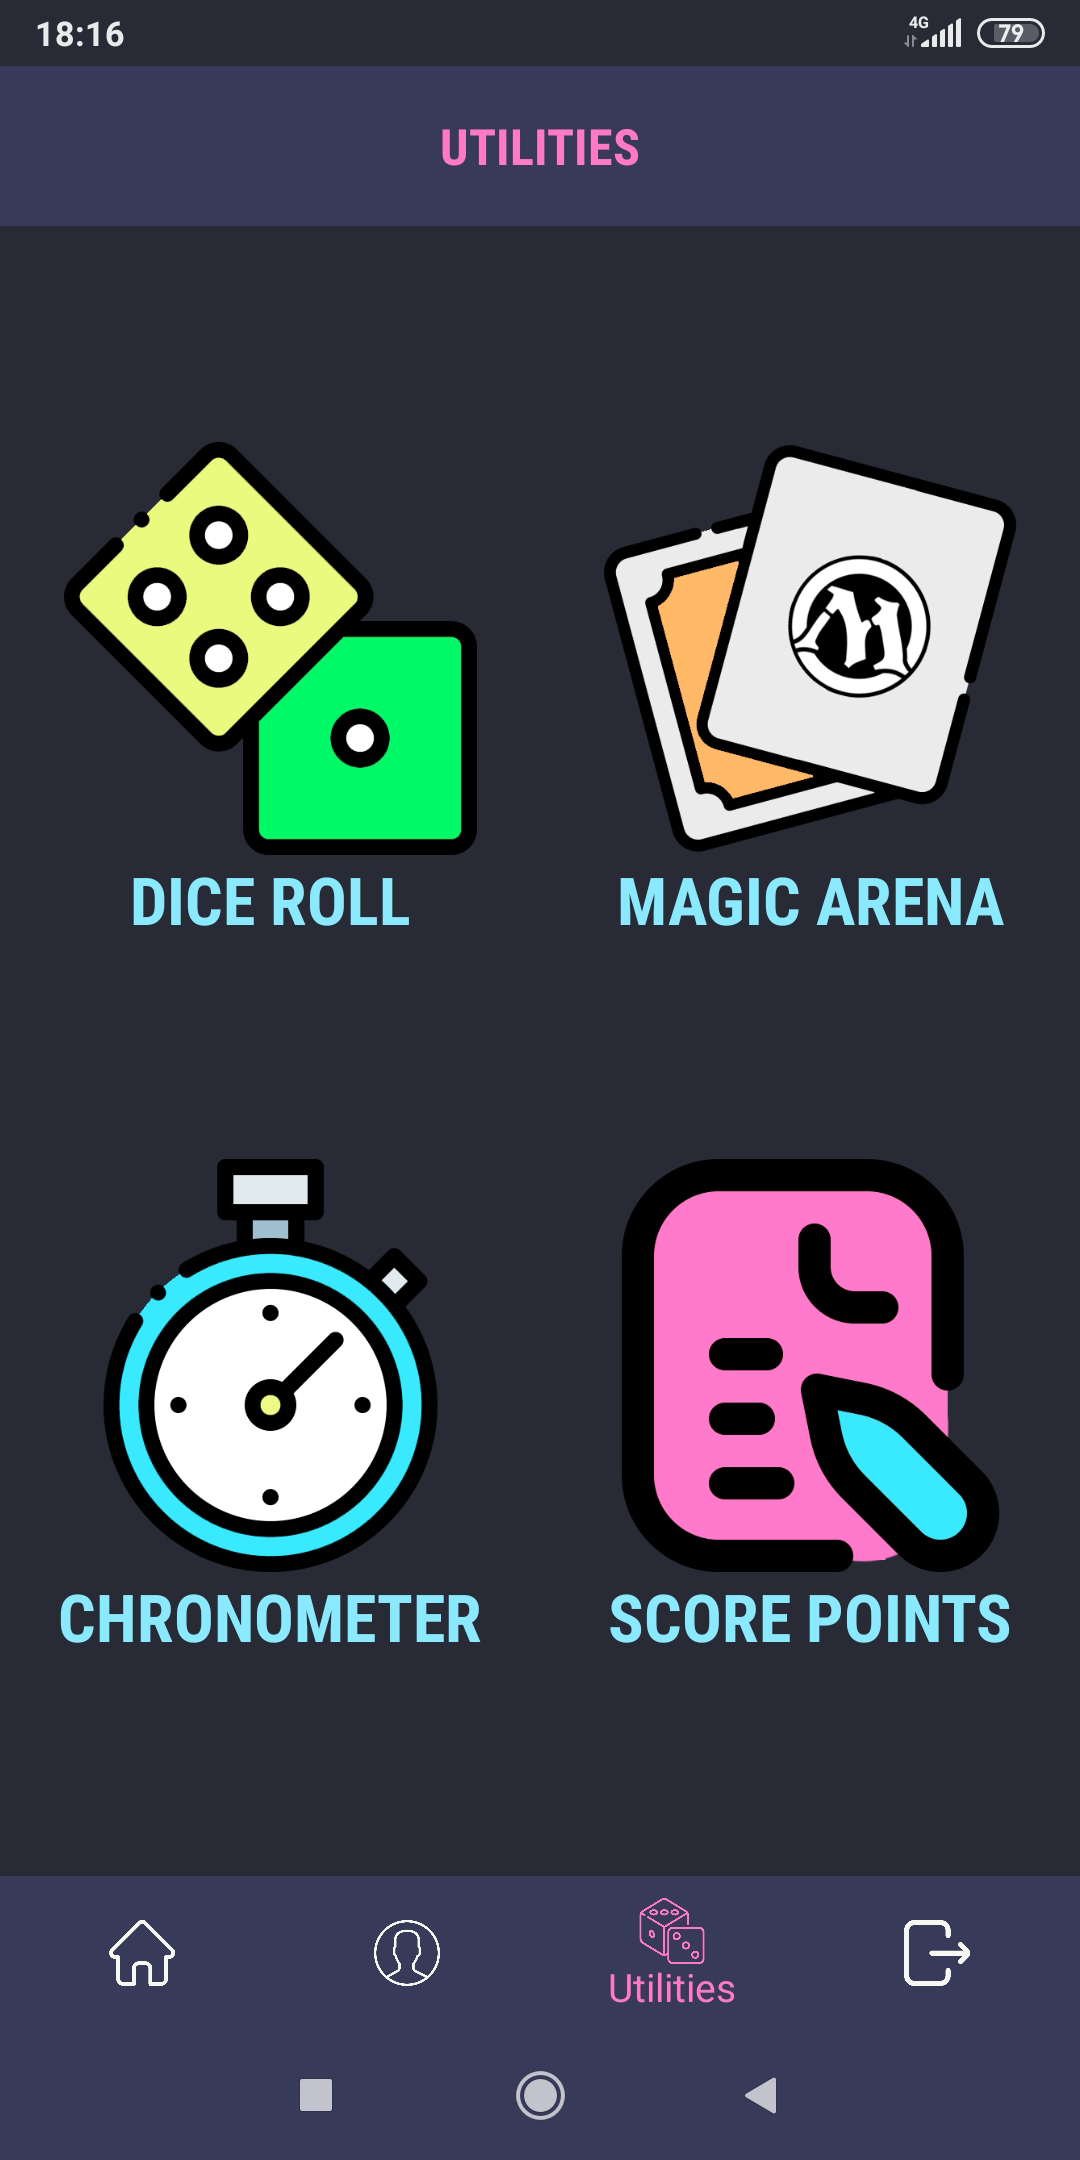
\includegraphics[width=0.3\linewidth]{fig/Uso/26.png}
    \caption{Ventana de utilidades}
    \label{fig:uso26}
\end{figure}

Dichas utilidades serán accesibles mediante 4 imágenes.

\begin{figure}[H]
    \centering
    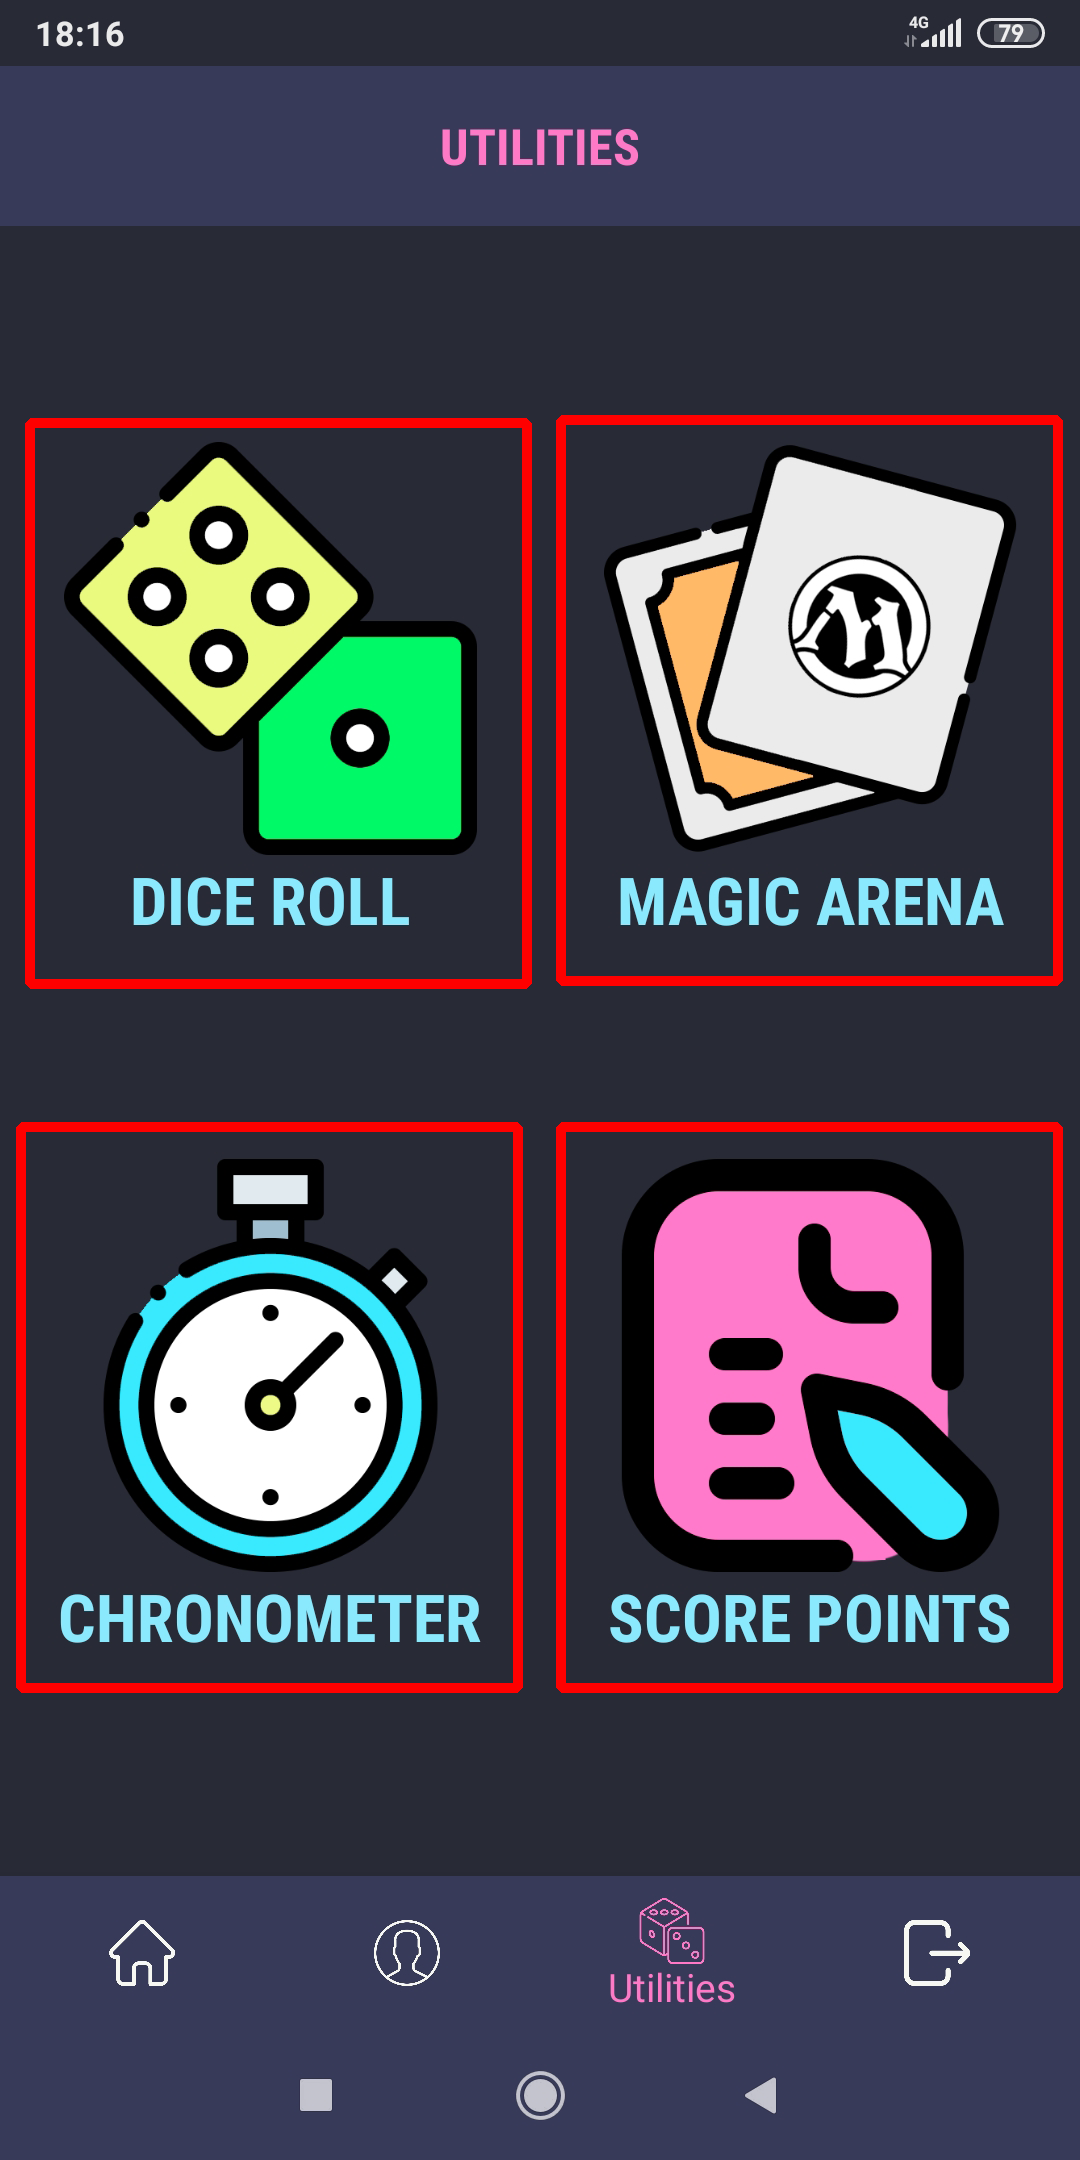
\includegraphics[width=0.3\linewidth]{fig/Uso/27.png}
    \caption{Accesos a las utilidades}
    \label{fig:uso27}
\end{figure}

Como primera utilidad tenemos \textit{Lanzamiento de dados}, que, como bien describe su nombre, sirve para lanzar dados. El número de dados y el tipo de dados se pueden ajustar mediante los botones que tendremos en la zona superior de la ventana.

\begin{figure}[H]
    \centering
    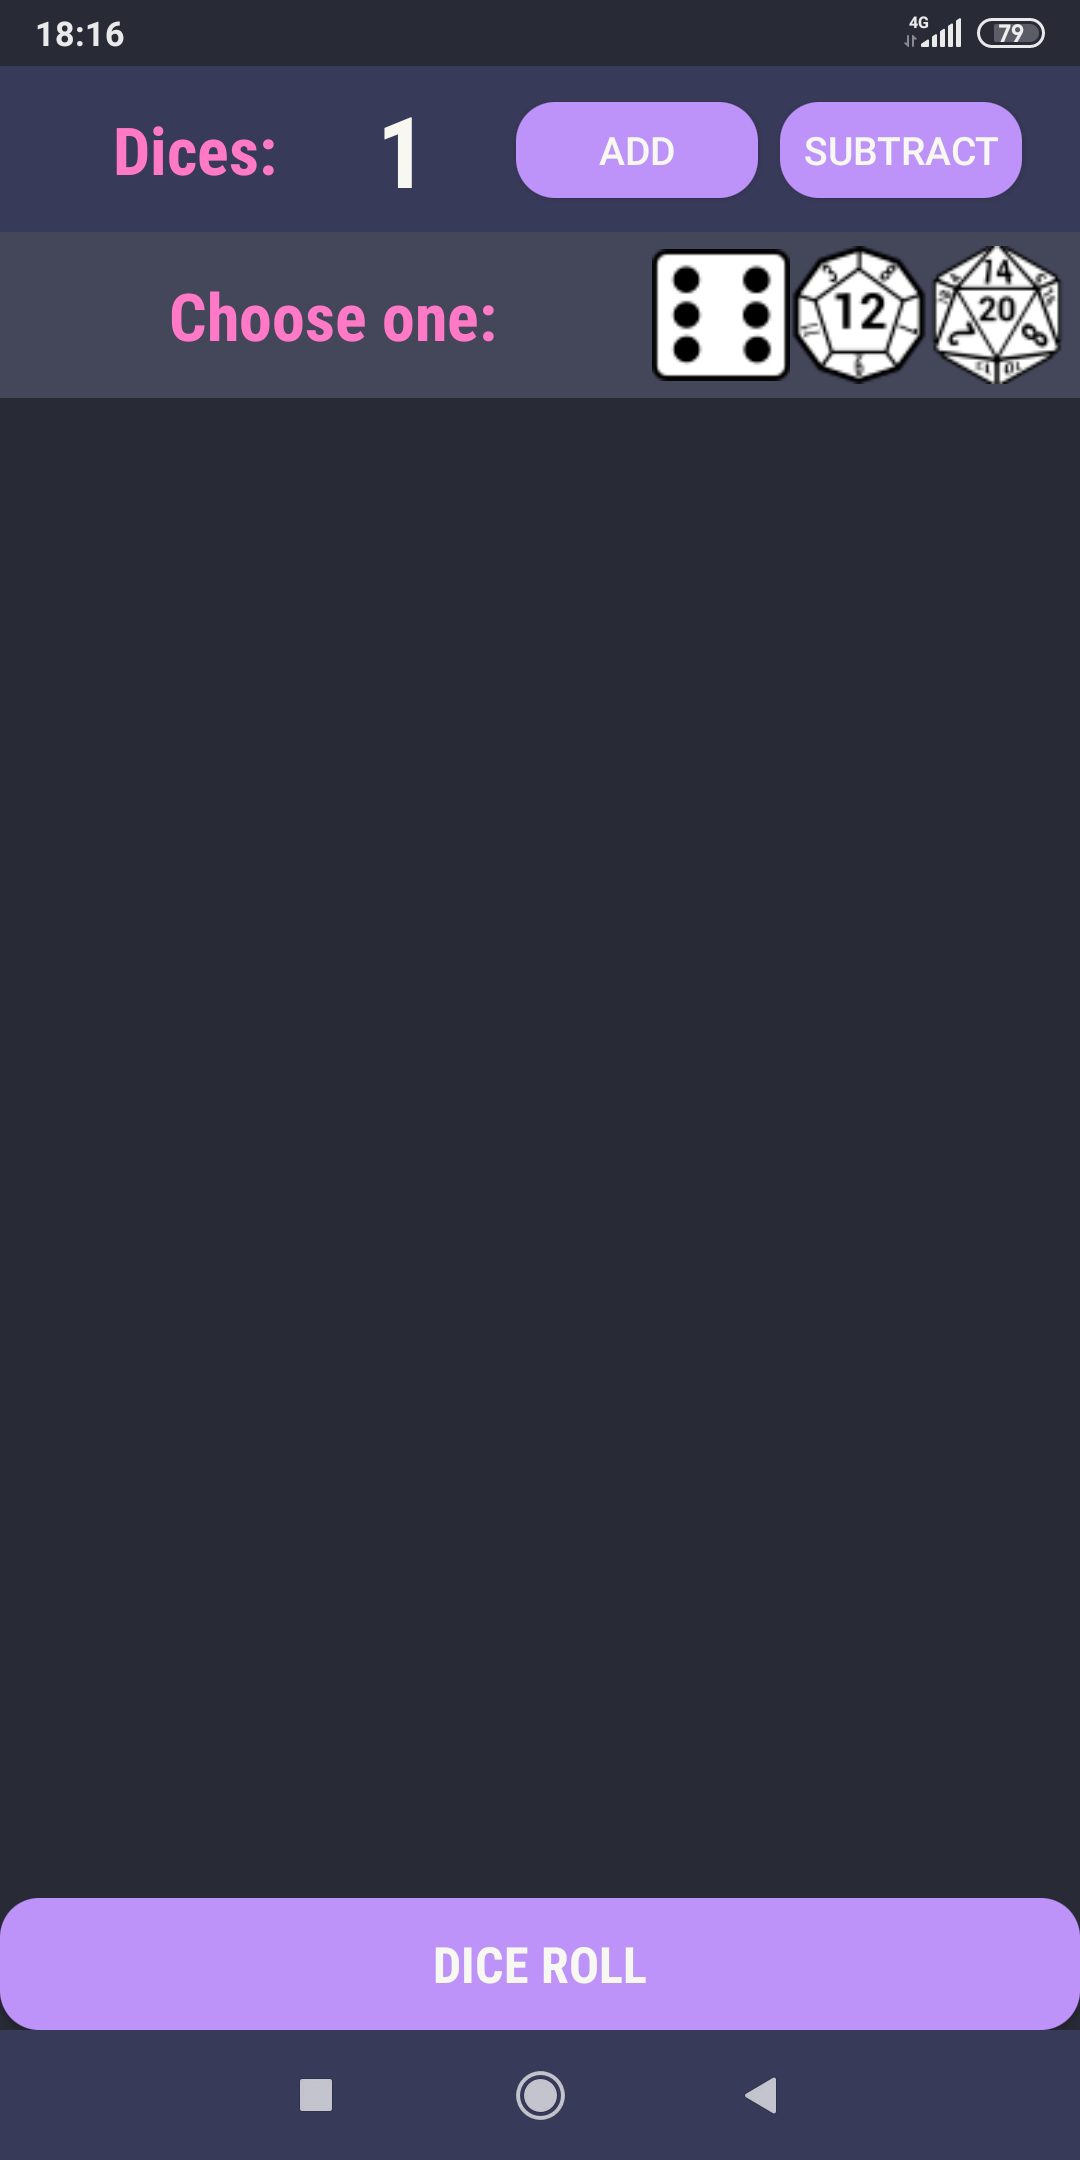
\includegraphics[width=0.3\linewidth]{fig/Uso/28.png}
    \caption{Lanzamiento de dados 1}
    \label{fig:uso28}
\end{figure}

Una vez lancemos los dados, se nos mostrará una lista con distintas caras del dado tantas veces como hayamos elegido anteriormente. Esta lista también tiene la capacidad de hacer scroll.

\begin{figure}[H]
    \centering
    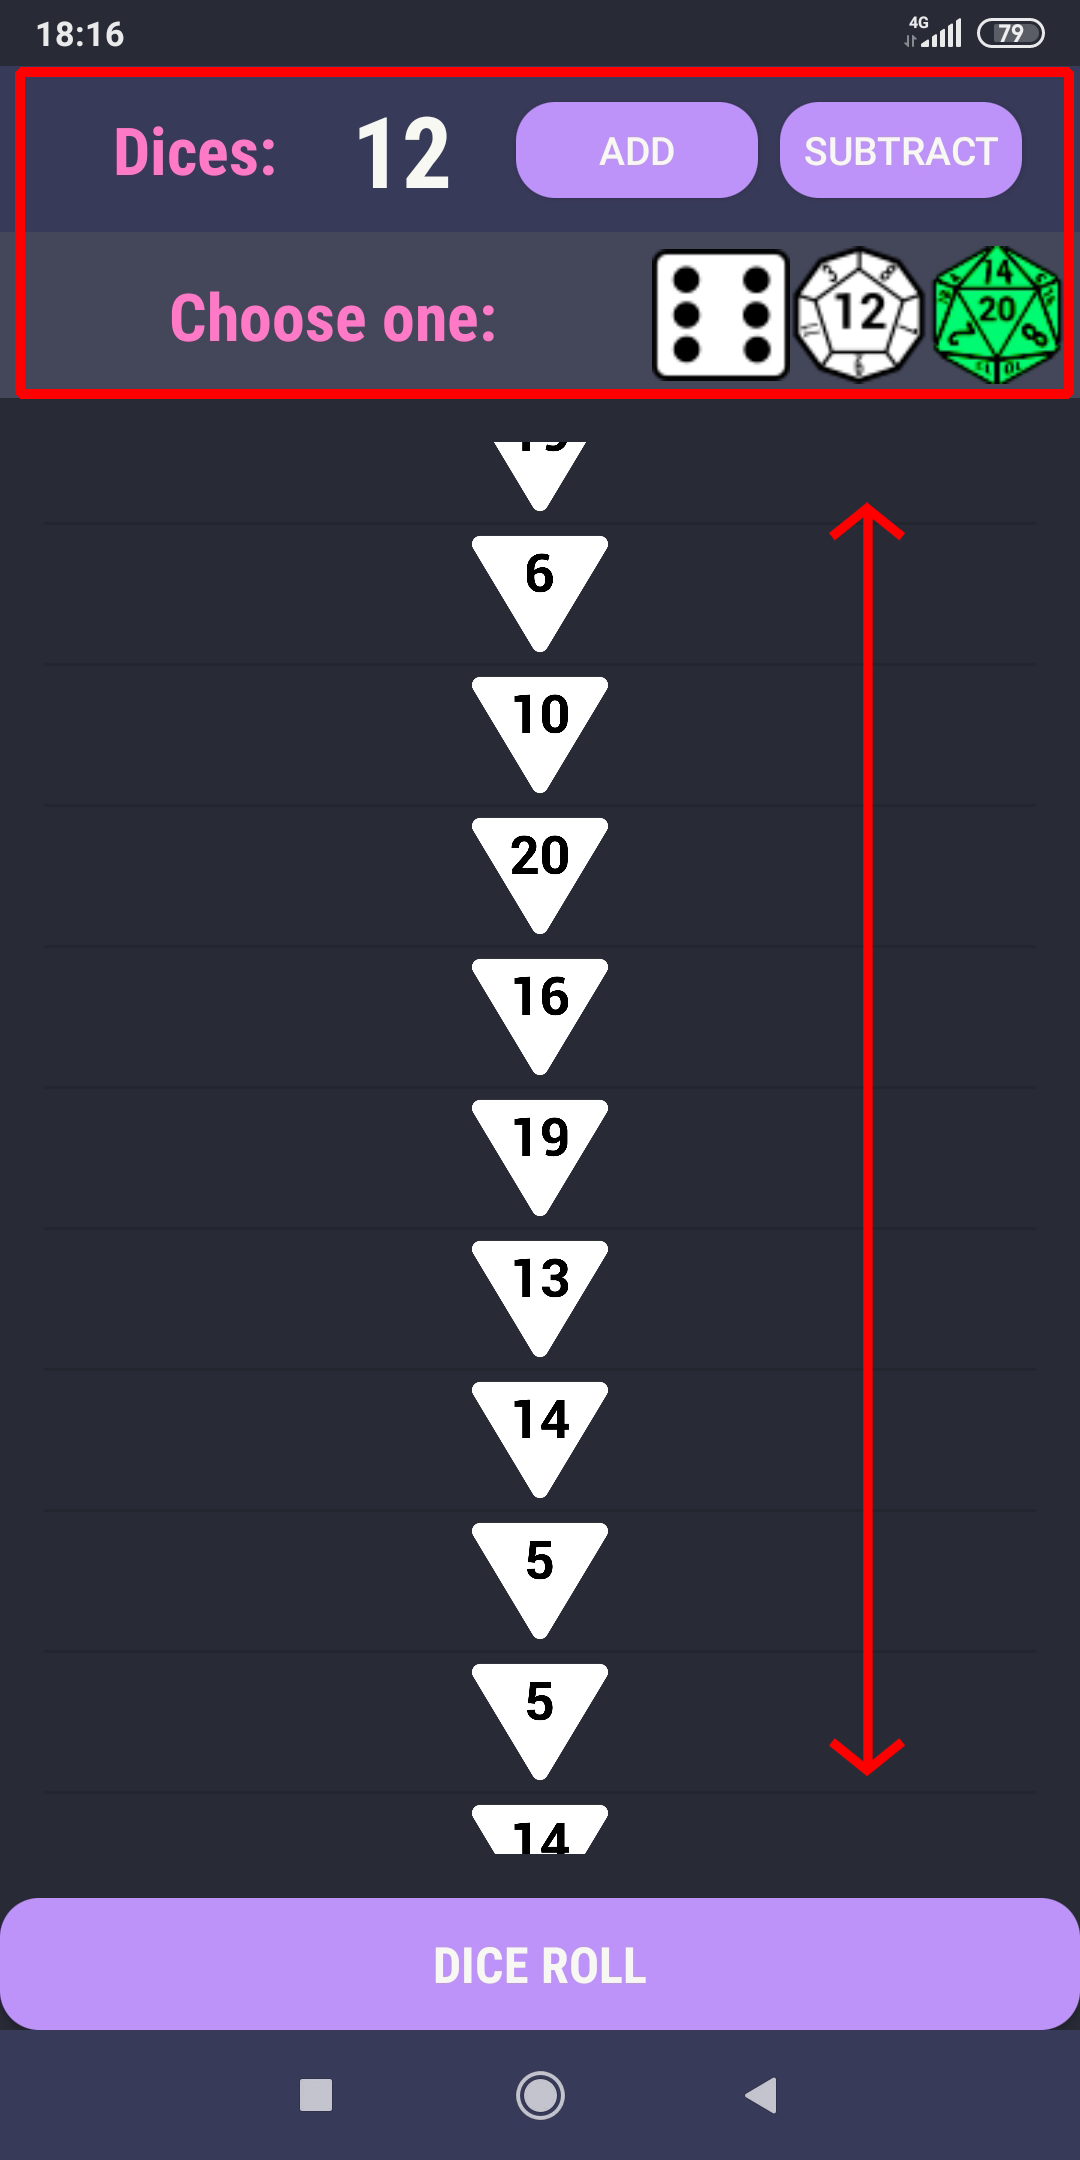
\includegraphics[width=0.3\linewidth]{fig/Uso/29.png}
    \caption{Lanzamiento de dados 2}
    \label{fig:uso29}
\end{figure}

Como segunda utilidad tenemos \textit{Magic Arena} donde se nos facilitará una serie de contadores que se pueden aumentar y disminuir de uno en uno o de cinco en cinco. Estos contadores pueden representar salud, maná, veneno, ataque, commander, etc. Todo esto depende del juego al que se esté jugando.

\begin{figure}[H]
    \centering
    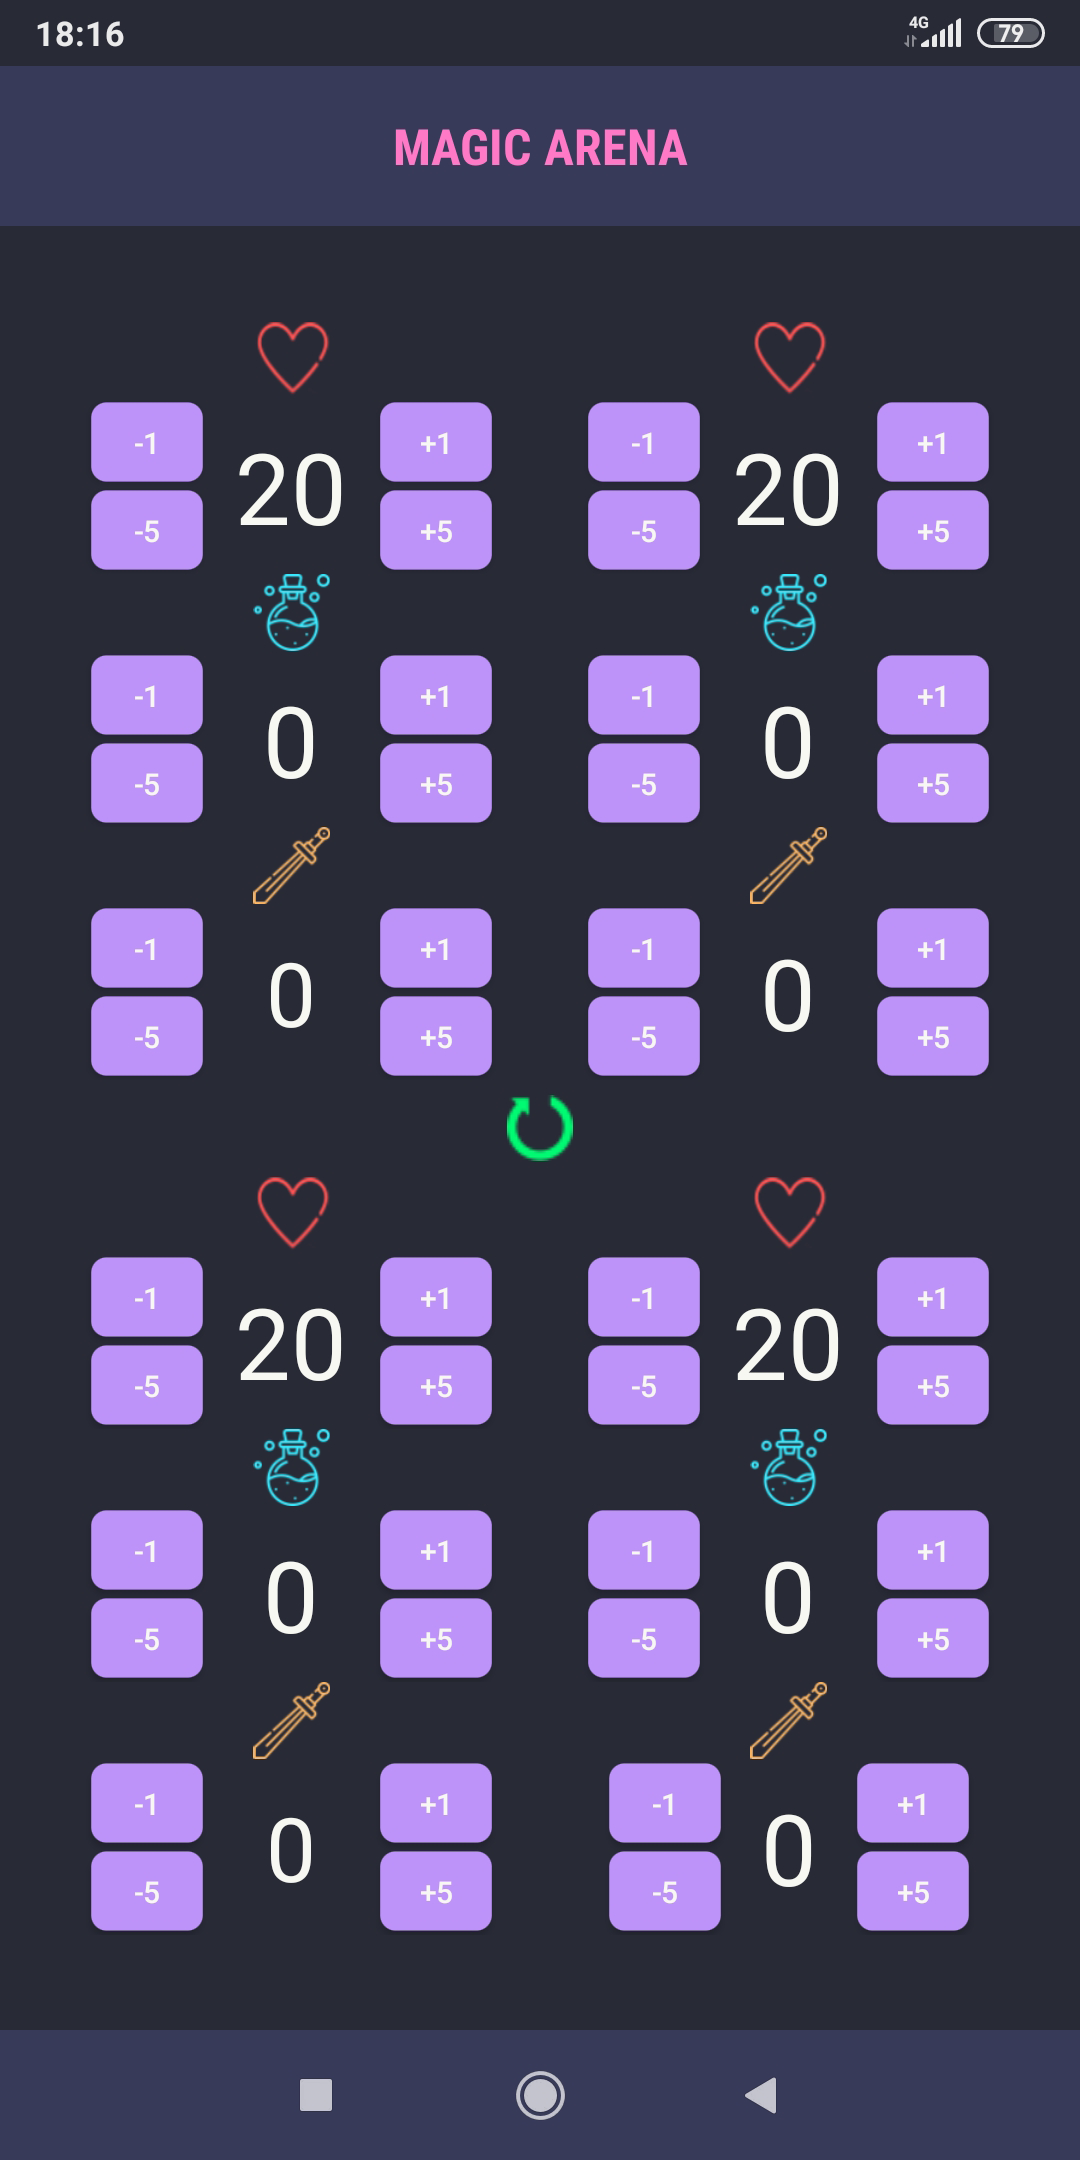
\includegraphics[width=0.3\linewidth]{fig/Uso/30.png}
    \caption{Magic Arena 1}
    \label{fig:uso30}
\end{figure}

\begin{figure}[H]
    \centering
    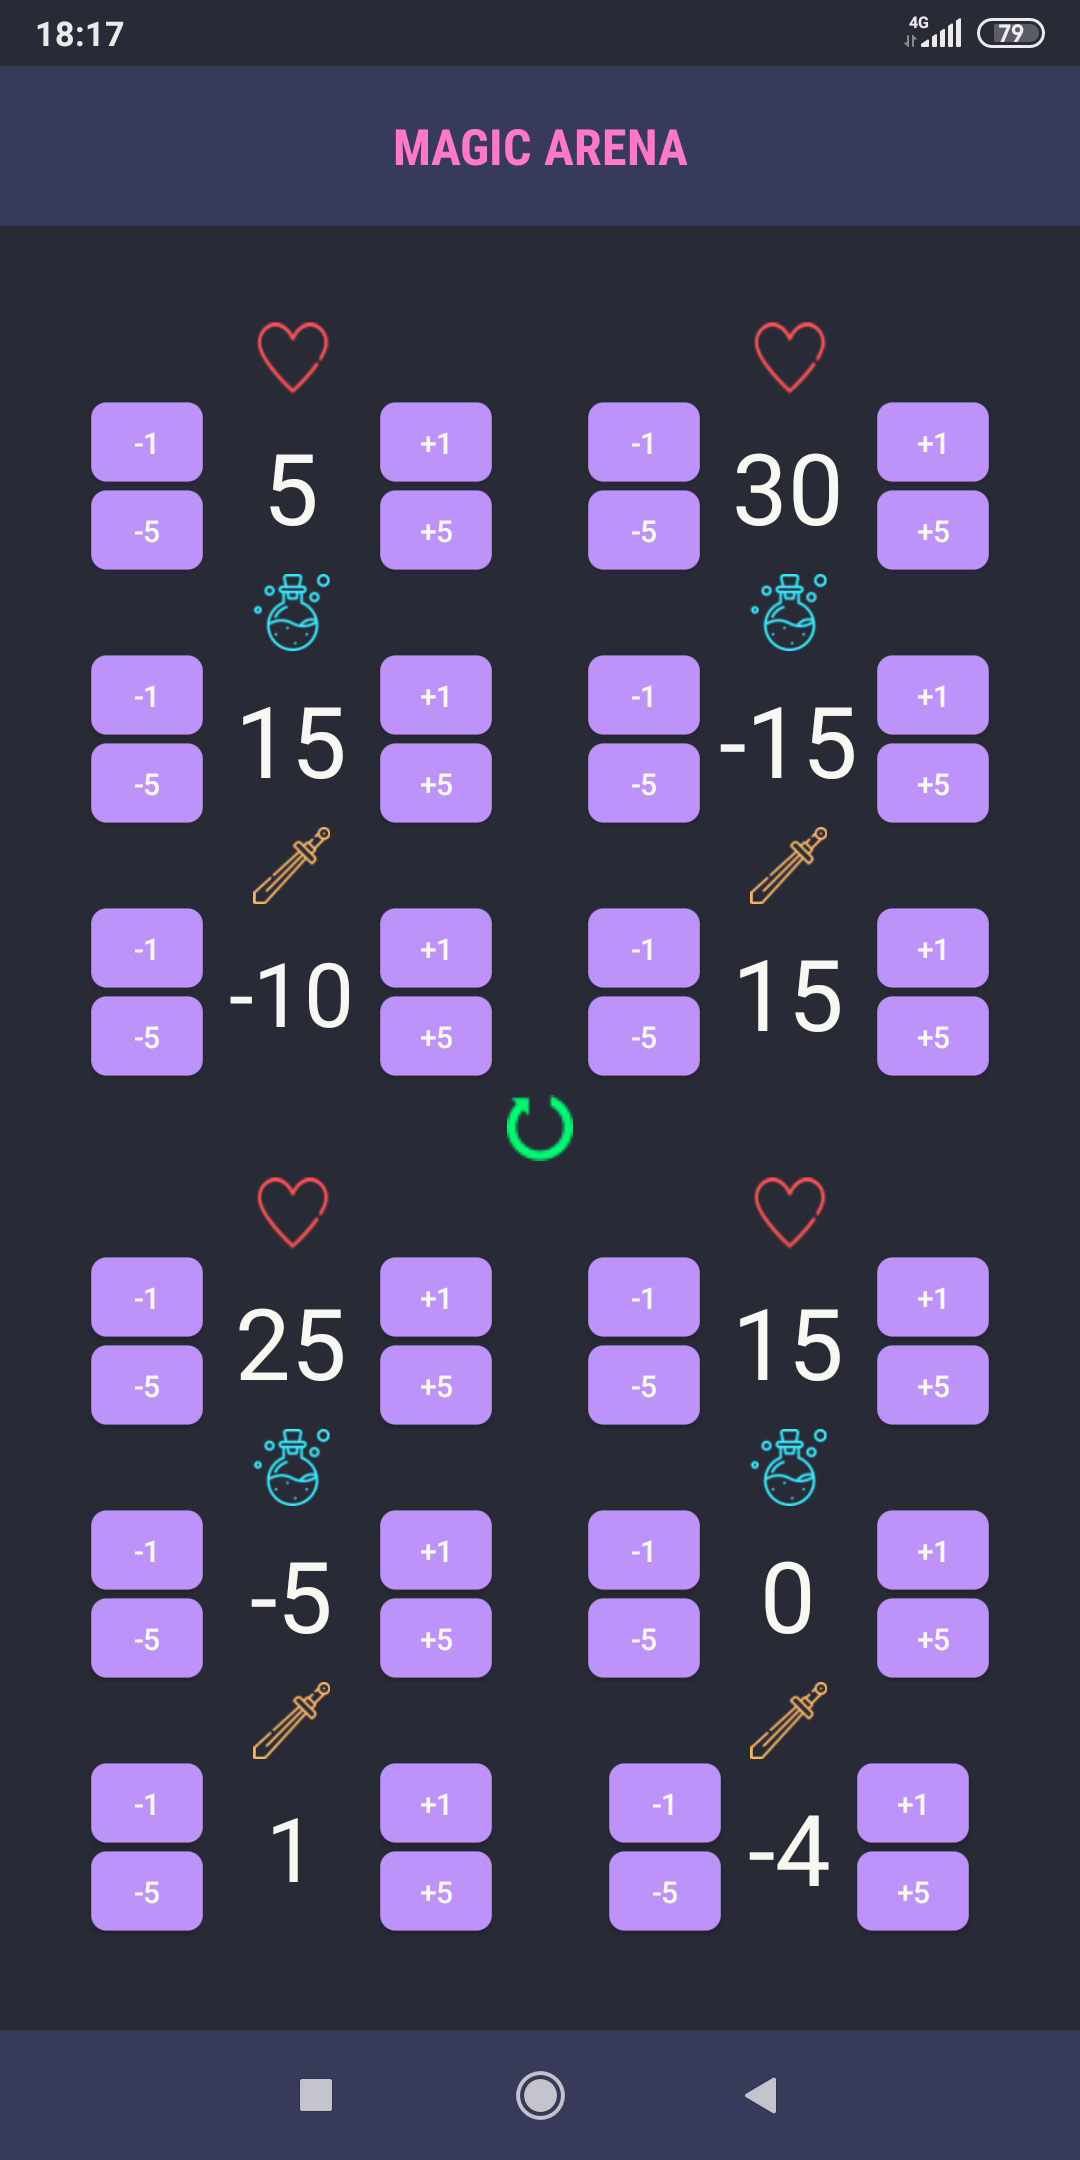
\includegraphics[width=0.3\linewidth]{fig/Uso/31.png}
    \caption{Magic Arena 2}
    \label{fig:uso31}
\end{figure}

Estos contadores se pueden restablecer sin salir de la utilidad haciendo clic sobre el botón que nos encontramos en el centro.

\begin{figure}[H]
    \centering
    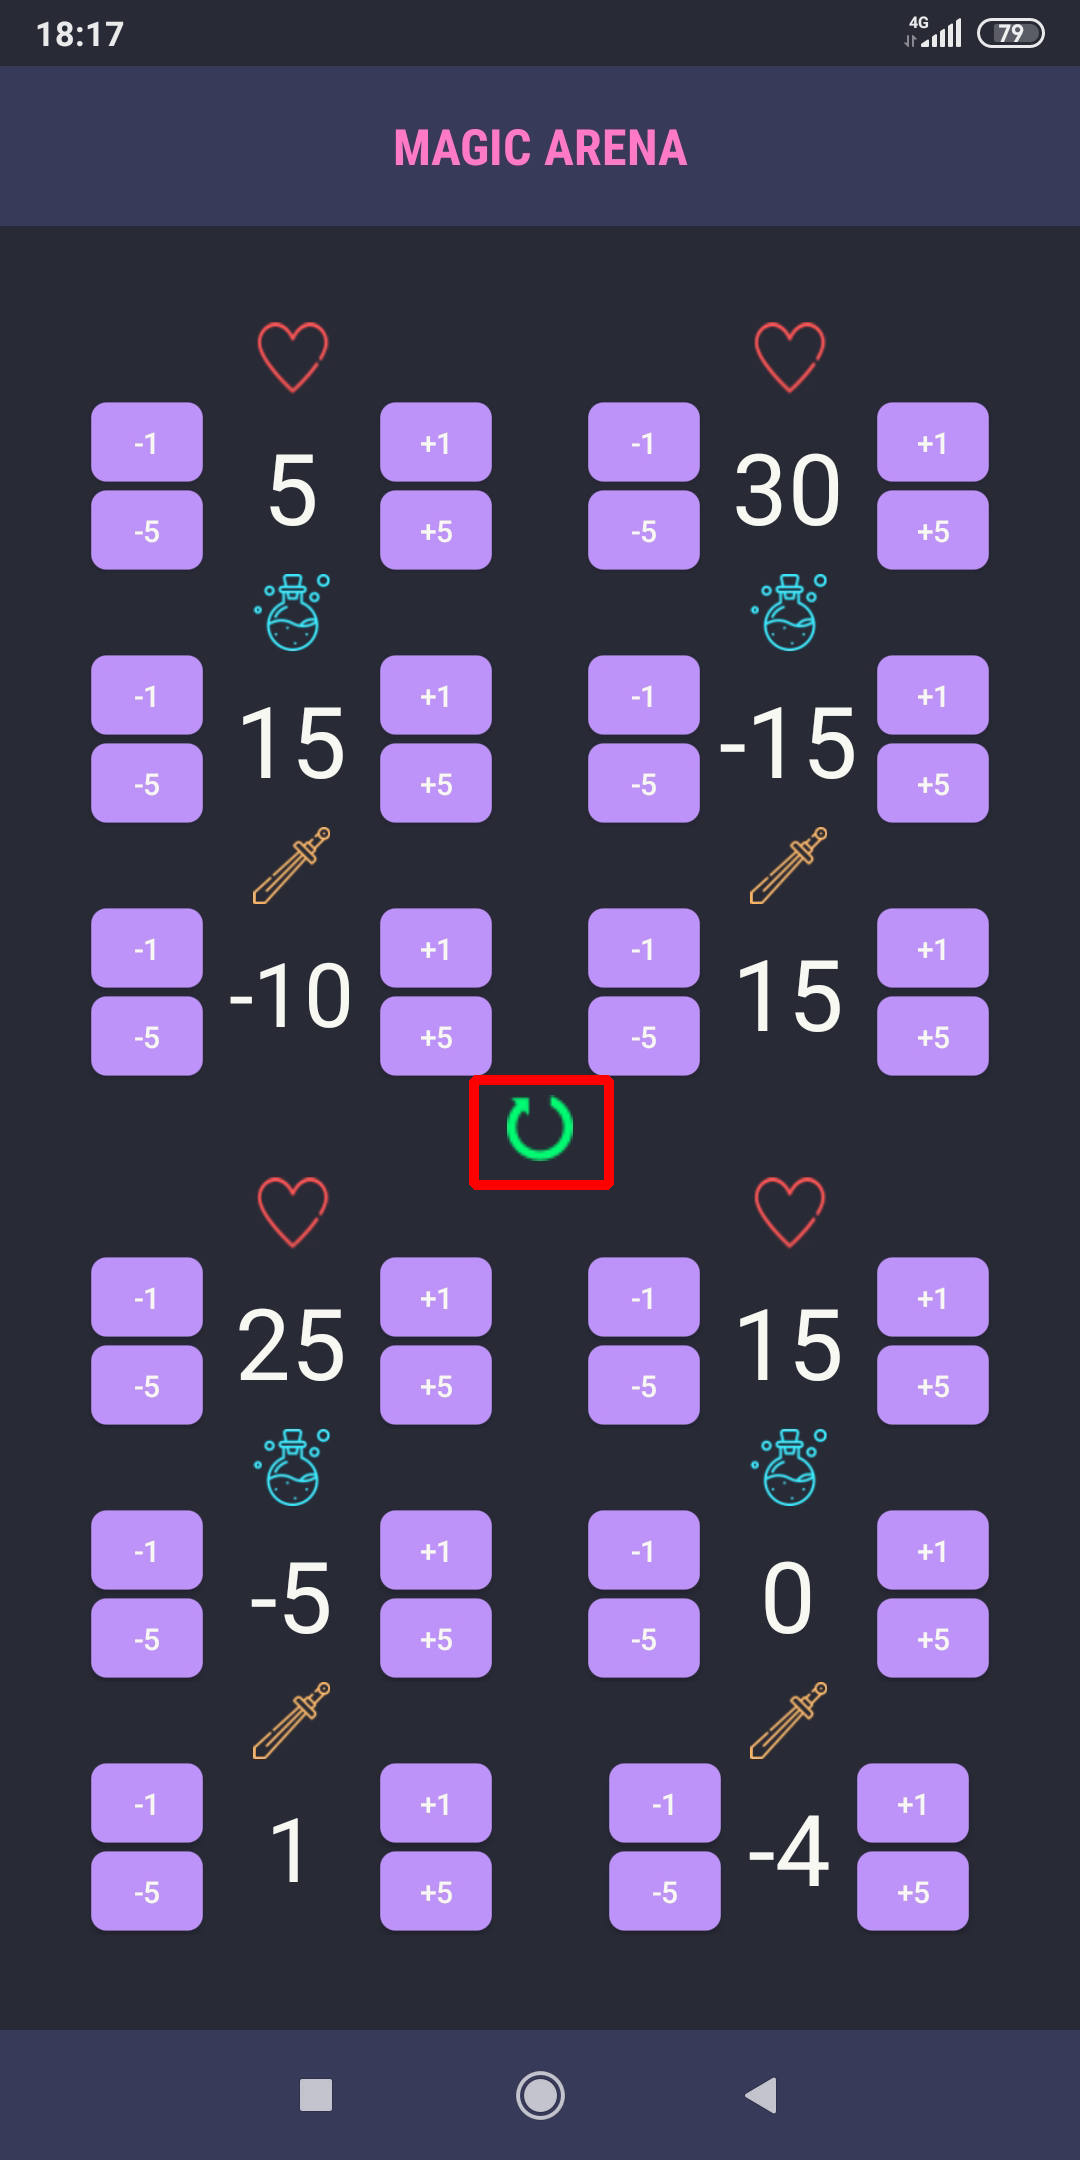
\includegraphics[width=0.3\linewidth]{fig/Uso/32.png}
    \caption{Magic Arena 3}
    \label{fig:uso32}
\end{figure}

De penúltima utilidad nos encontraremos con un simple cronómetro el cual hace la función de cronómetro: calcular el tiempo transcurrido.

En esta actividad habrá tres botones los cuales sirven para iniciar, pausar o reiniciar el tiempo.

\begin{figure}[H]
    \centering
    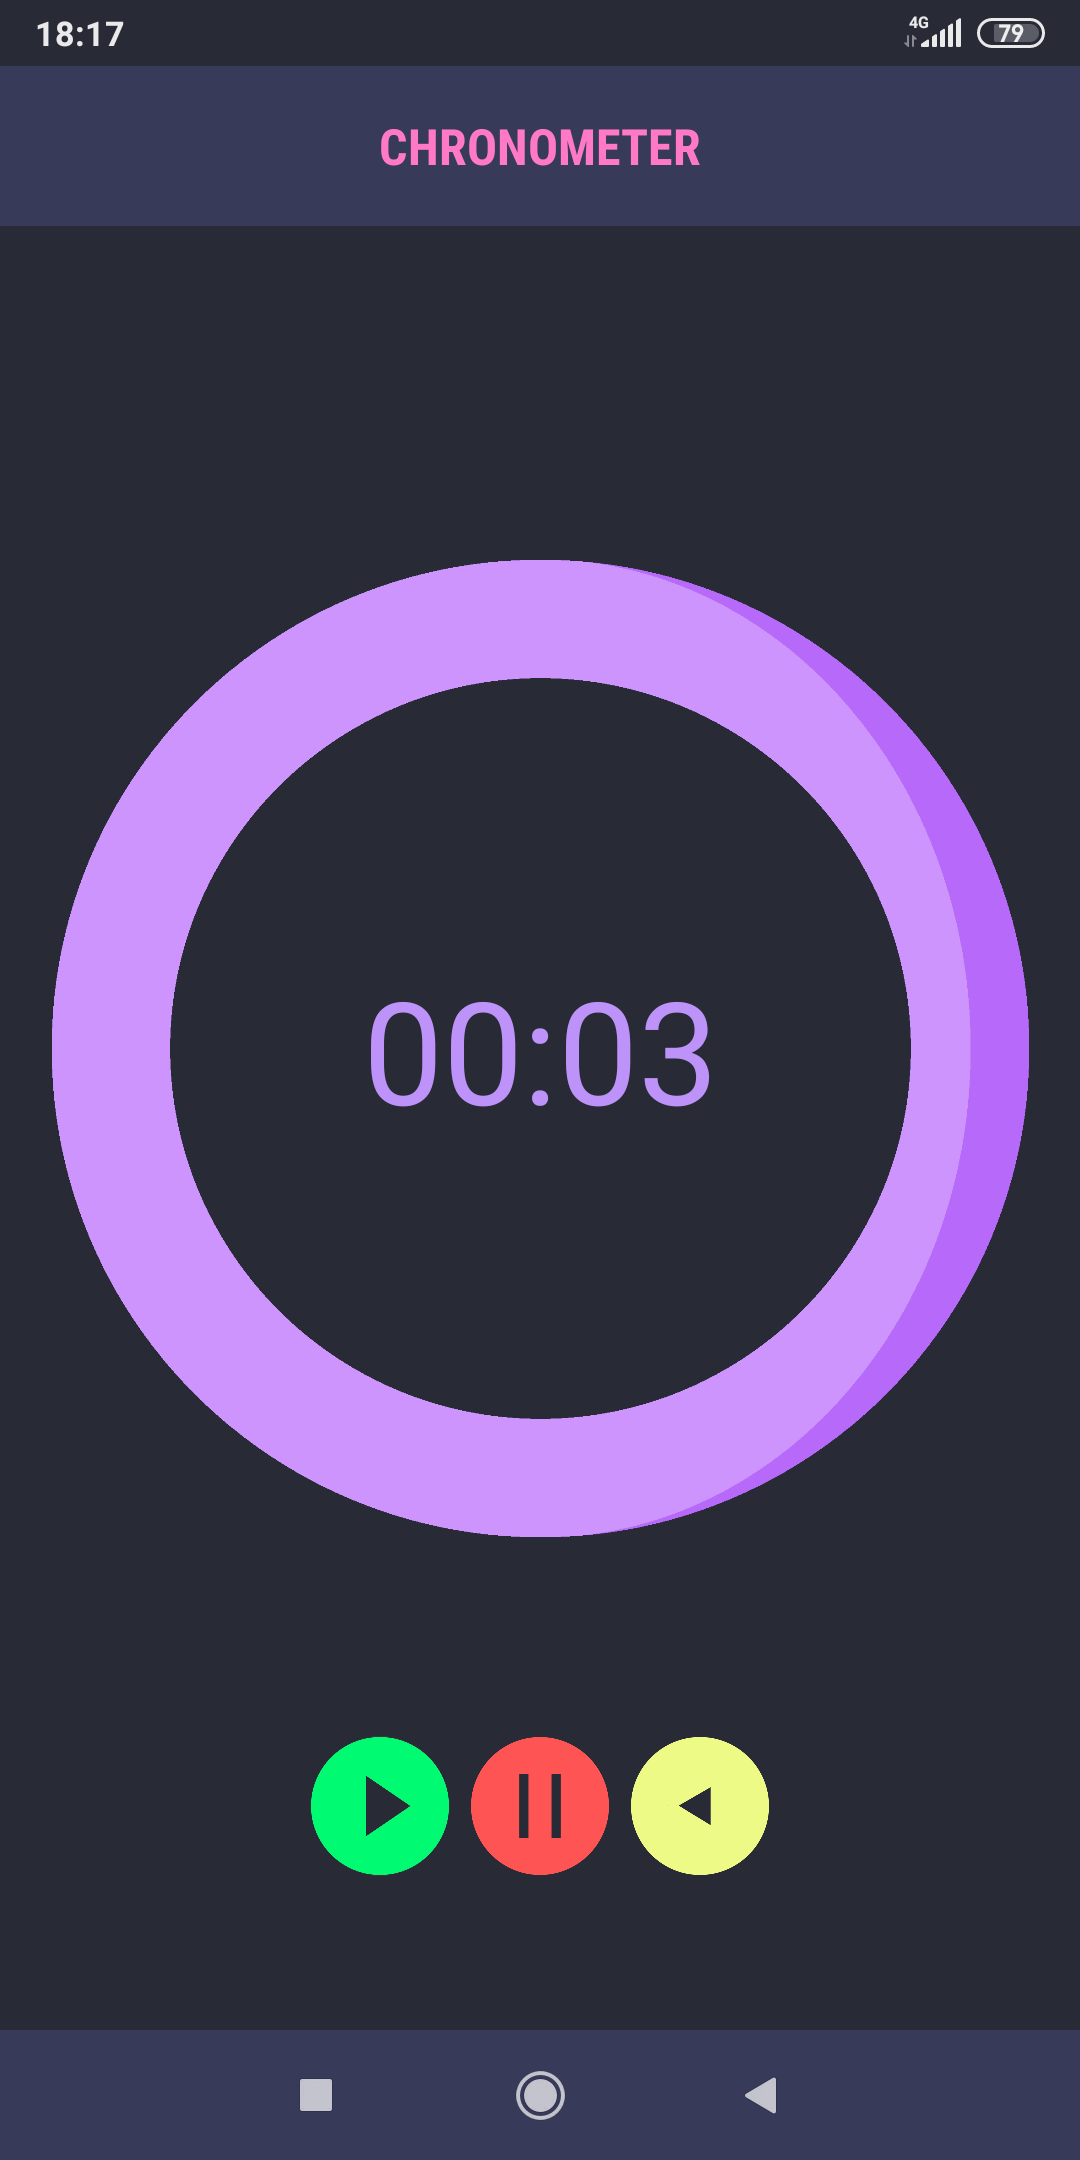
\includegraphics[width=0.3\linewidth]{fig/Uso/33.png}
    \caption{Cronómetro 1}
    \label{fig:uso33}
\end{figure}

\begin{figure}[H]
    \centering
    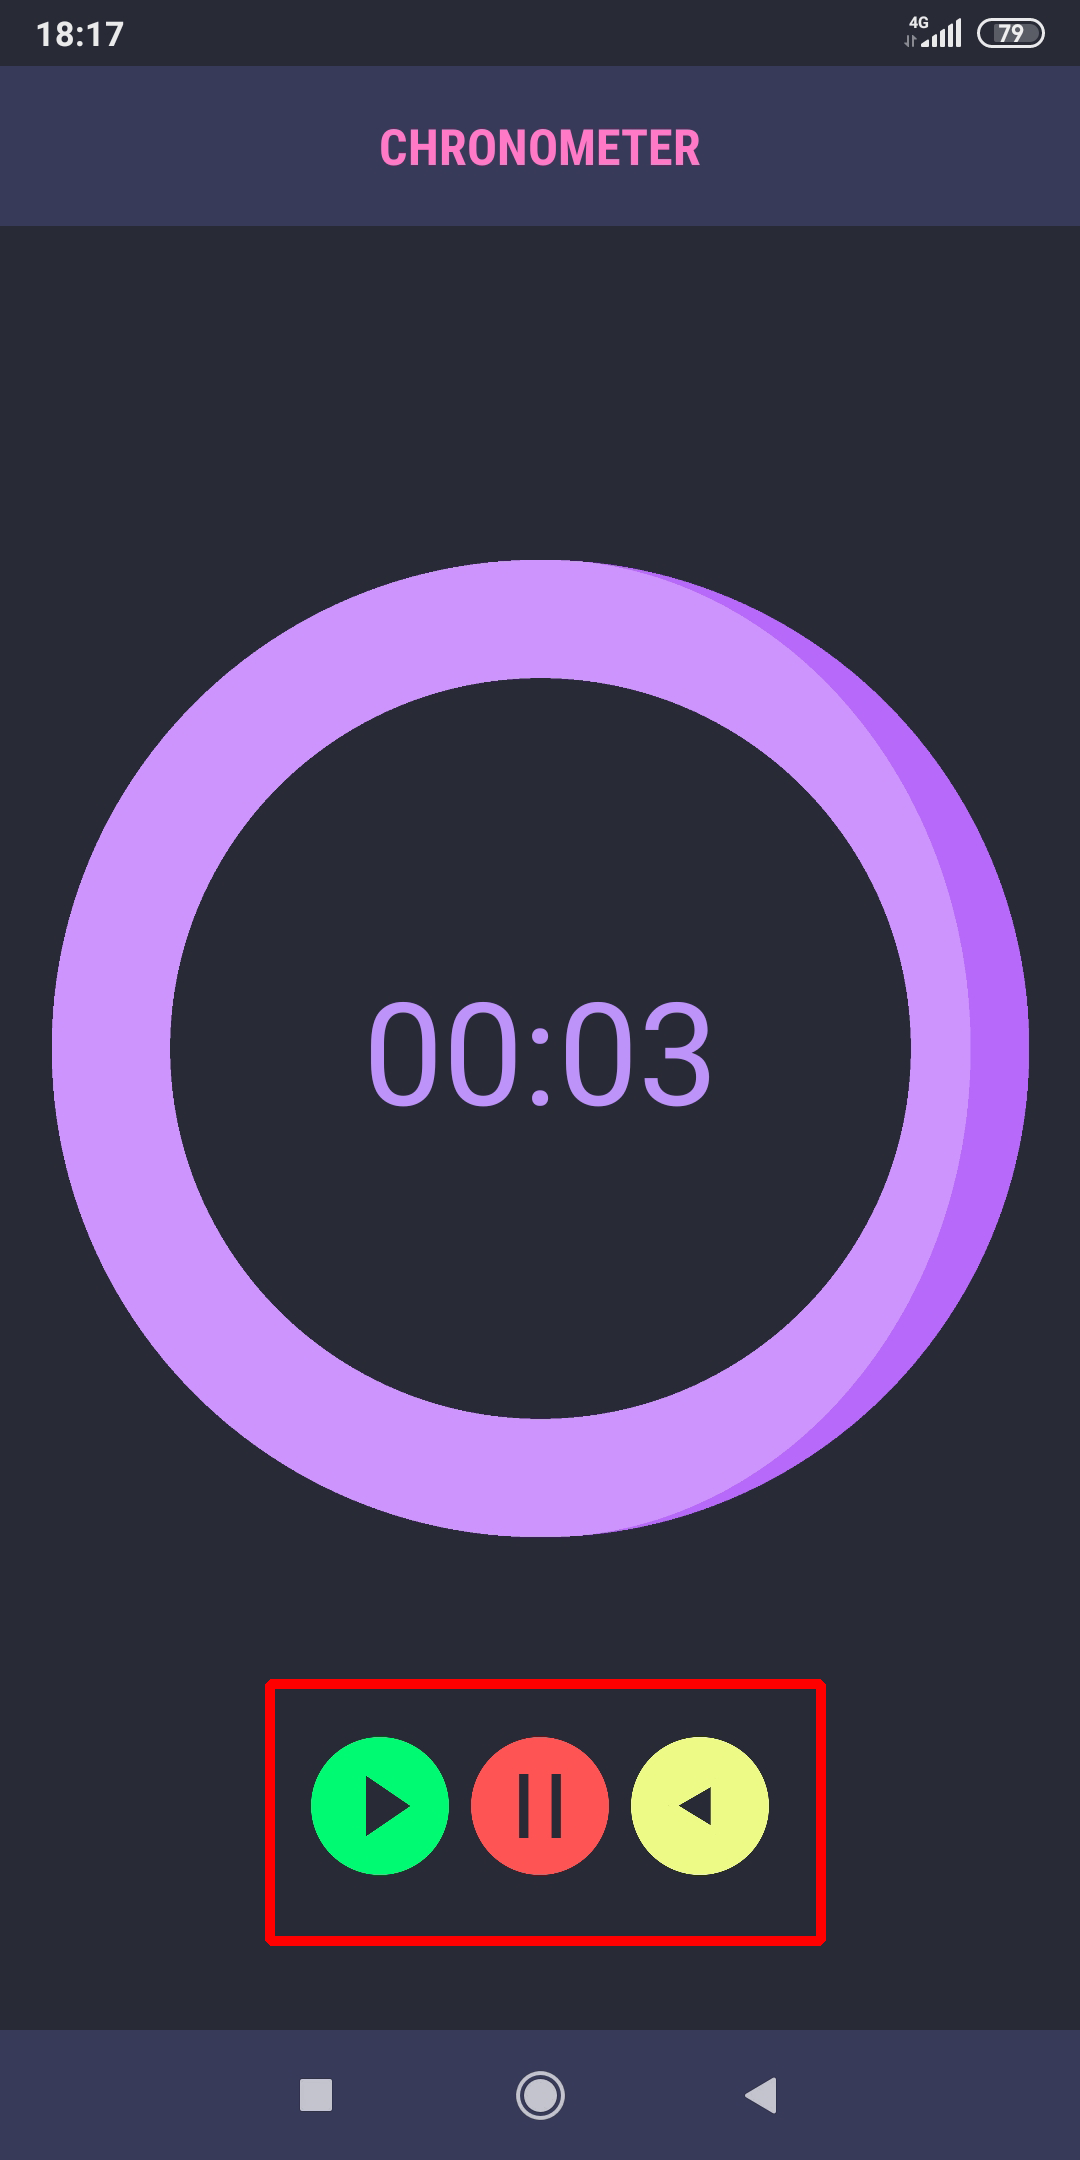
\includegraphics[width=0.3\linewidth]{fig/Uso/34.png}
    \caption{Cronómetro 2}
    \label{fig:uso34}
\end{figure}

Y de última utilidad está el \textit{registrador de puntos}. Aquí nos encontraremos con un texto que podremos modificar a un número comprendido entre 1 a 30 que especificará el número de jugadores en la partida, con lo que aparecerá, el mismo número de veces marcado, dos textos a modificar y dos botones. En estos textos tendremos que poner el nombre del jugador y su puntuación en \textit{vivo}, esto quiere decir durante el transcurso de la partida ir modificándolo. La puntuación puede ser escrita a mano (con el teclado) o haciendo uso de los botones que se proporcionan para sumar o restar de uno en uno dichos puntos.

\begin{figure}[H]
    \centering
    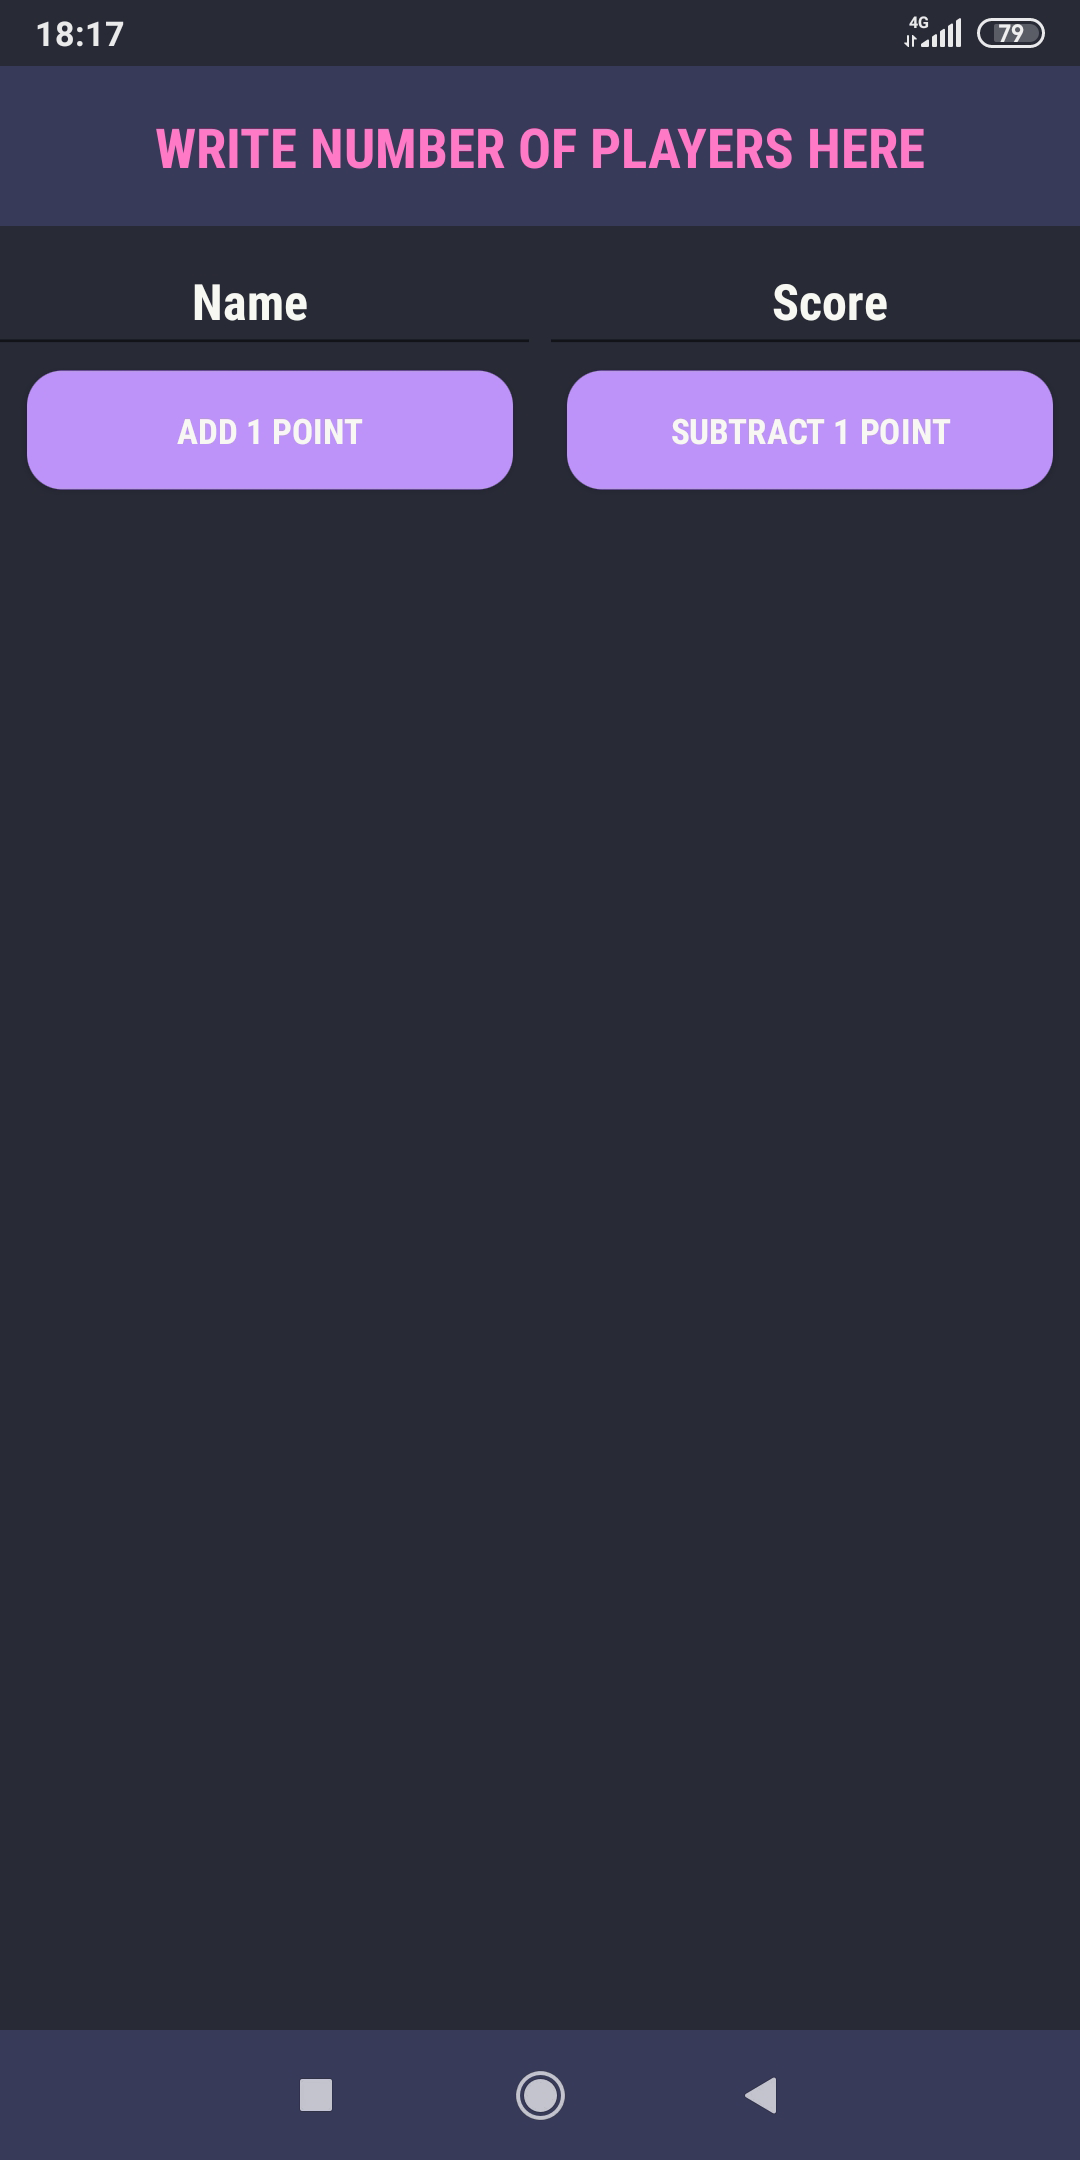
\includegraphics[width=0.3\linewidth]{fig/Uso/35.png}
    \caption{Registrador de puntos 1}
    \label{fig:uso35}
\end{figure}

\begin{figure}[H]
    \centering
    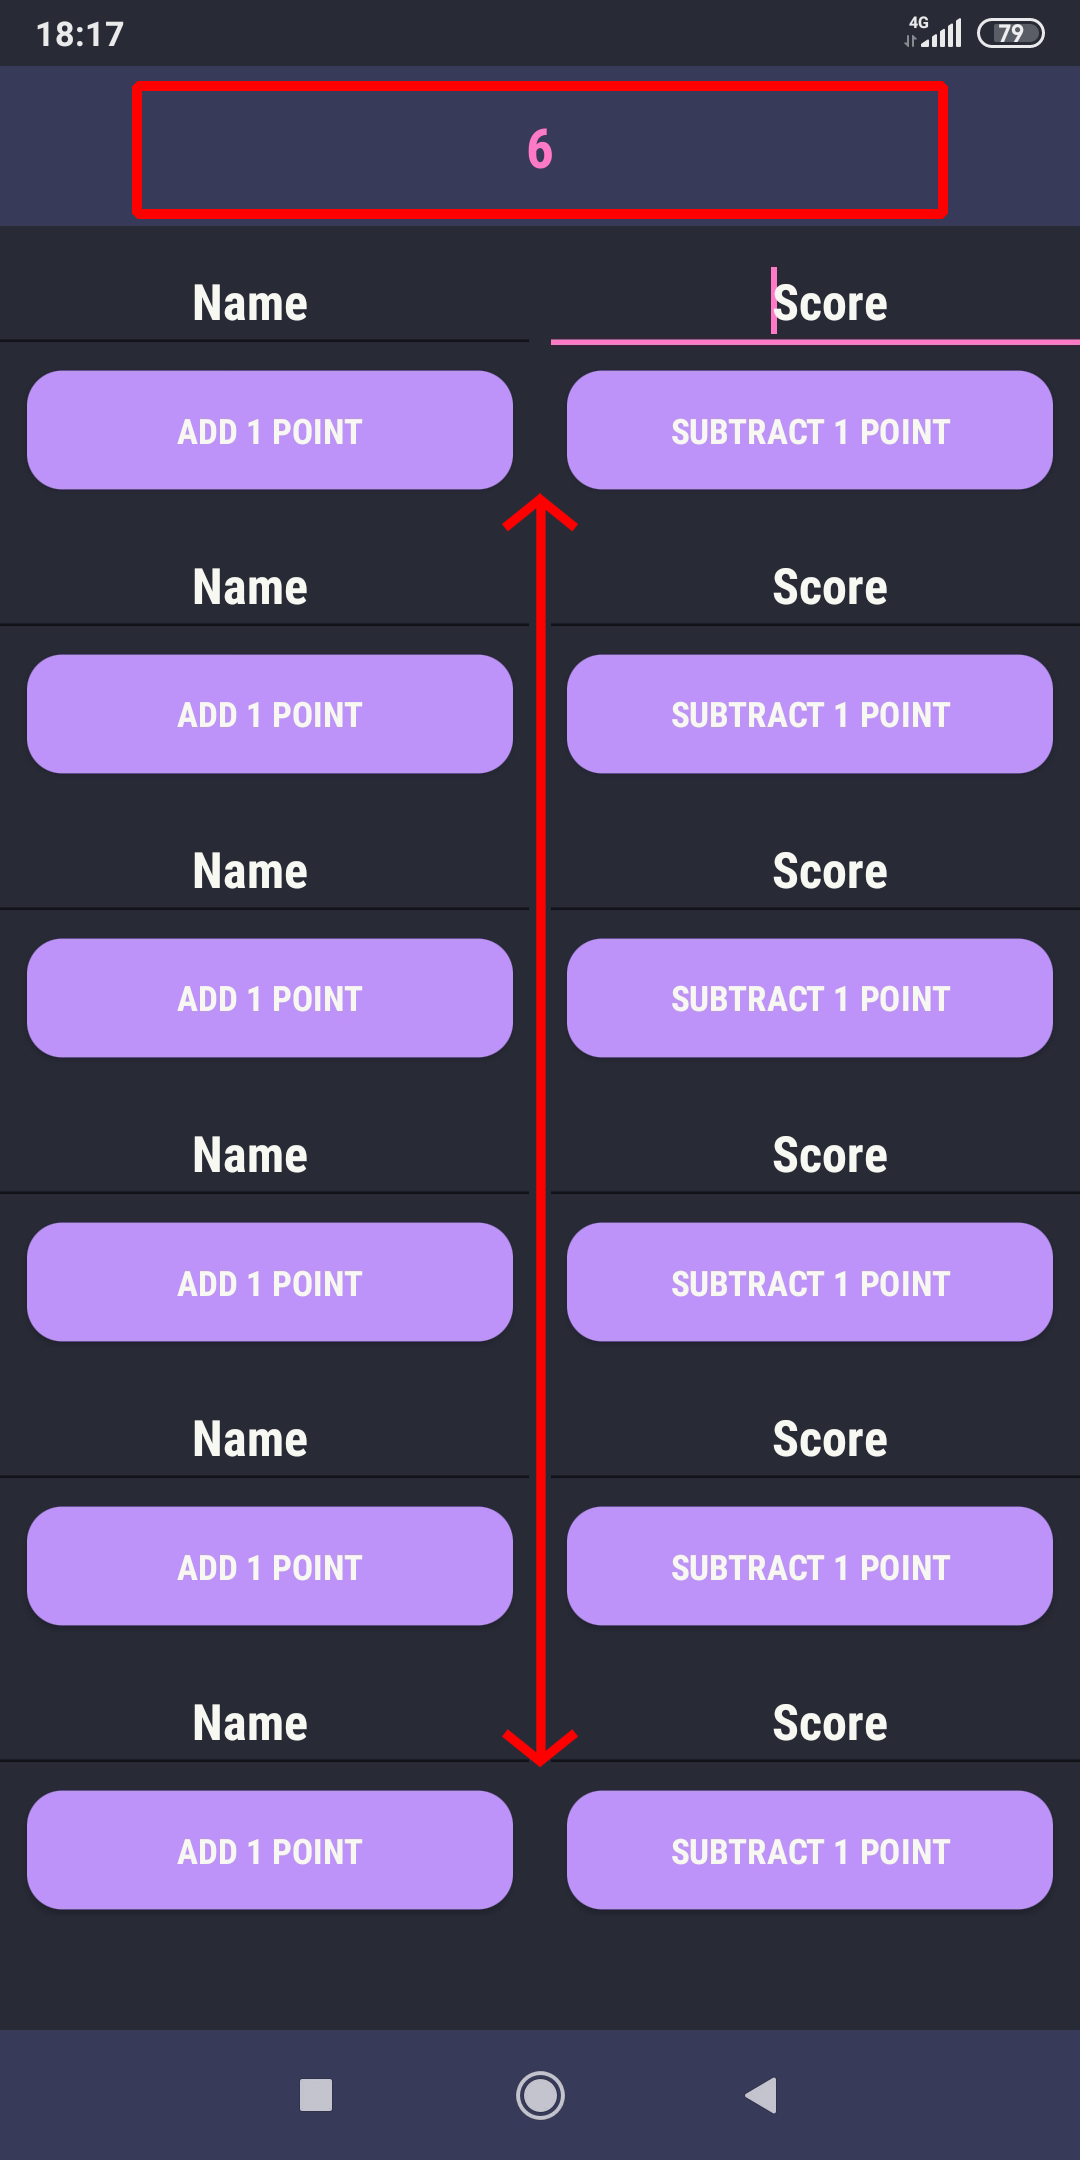
\includegraphics[width=0.3\linewidth]{fig/Uso/36.png}
    \caption{Registrador de puntos 2}
    \label{fig:uso36}
\end{figure}

\begin{figure}[H]
    \centering
    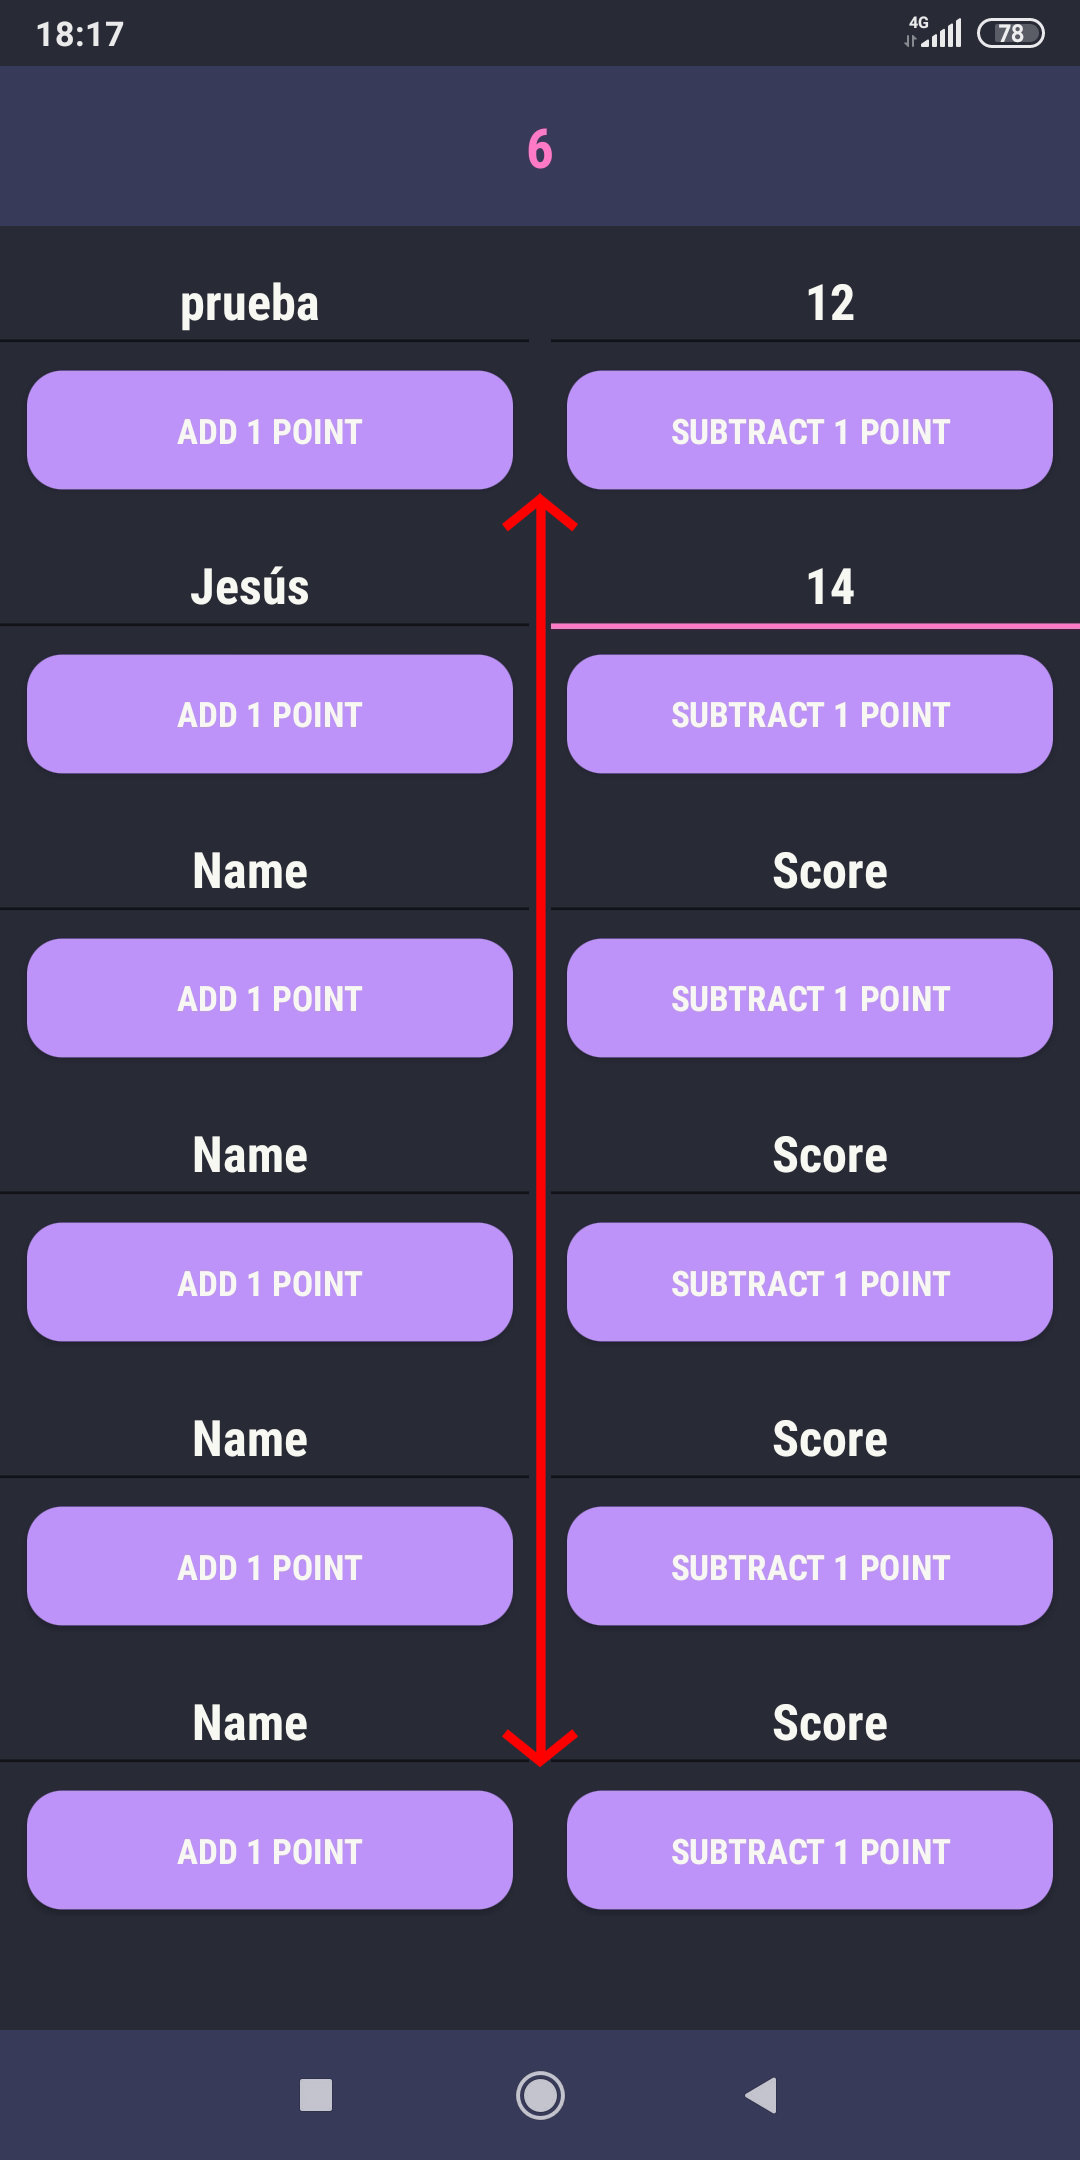
\includegraphics[width=0.3\linewidth]{fig/Uso/37.png}
    \caption{Registrador de puntos 3}
    \label{fig:uso37}
\end{figure}